\documentclass[12pt]{article}

%----------------------Autor y fecha----------------------

\title{Diseño de Sistemas}
\date{26 de mayo de 2019i}


%------------------------Paquetes-------------------------

\usepackage{graphicx}			% Gráficos
\usepackage[utf8]{inputenc}		% Codificación
\usepackage[spanish]{babel}		% Idioma
\usepackage{lastpage}
\usepackage{dcolumn}			% Tablas
\usepackage{enumitem}			% Listas
\usepackage{bm}					% Negrita en ecuaciones
%\usepackage{pstricks}			% Arboles
%\usepackage{pst-tree}			% 
\usepackage{amsmath,caption,booktabs}
\usepackage{amssymb}




\graphicspath{ {./Imagenes/} }
%---------------------------------------------------------

%------------------------Márgenes-------------------------

\usepackage{vmargin}
\setpapersize{A4}
\setmargins{3cm}	% margen izquierdo
{1.25cm}			% margen superior
{16.5cm}			% anchura del texto
{24.2cm}			% altura del texto
{18pt}				% altura de los encabezados
{1cm}				% espacio entre el texto y los encabezados
{10pt}				% altura del pie de página
{2cm}				% espacio entre el texto y el pie de página
%---------------------------------------------------------

%-----------Tamaño de Encabezado y Pie de pagina----------

\usepackage{fancyhdr}						% Paquete

\setlength{\headwidth}{\textwidth}
\setlength{\headheight}{28pt}
\setlength{\footskip}{1cm}
\renewcommand{\headrulewidth}{0.4pt}
\renewcommand{\footrulewidth}{1pt}

%---------------------------------------------------------

%---------------------Diseño Encabezado-------------------

\fancyhead[L]{
\includegraphics[height=.5cm]{./logos/UTN-FRSF.jpg}}
\fancyhead[R]{\textsf{\Large{Ingeniería en Sistemas de Información}}}
%---------------------------------------------------------

%--------------------Diseño Pié de pagina-----------------


\fancyfoot[R] {\thepage \textnormal{ de} \pageref{LastPage}}
\fancyfoot[L]{Grupo 4A:\scriptsize{\textit{ Bode, Busso, Ferraro Trivelli, Storani}}}
\fancyfoot[C]{2019}
%---------------------------------------------------------



%\renewcommand{\familydefault}{\sfdefault}	% Cambio de fuente por defecto

\pagestyle{empty}							% Estilo de página (Habilita los encabezados y pié de página)




\begin{document}
\pagestyle{empty}		
\begin{titlepage}

\center
\end{titlepage}
\newpage
\pagestyle{fancy}

%%%%%%%%%%%%%%%%%%%%%%%
%%%%%%        CASO DE USO 1         %%%%%
%%%%%%%%%%%%%%%%%%%%%%%

\vfill
\begin{figure}[h!]
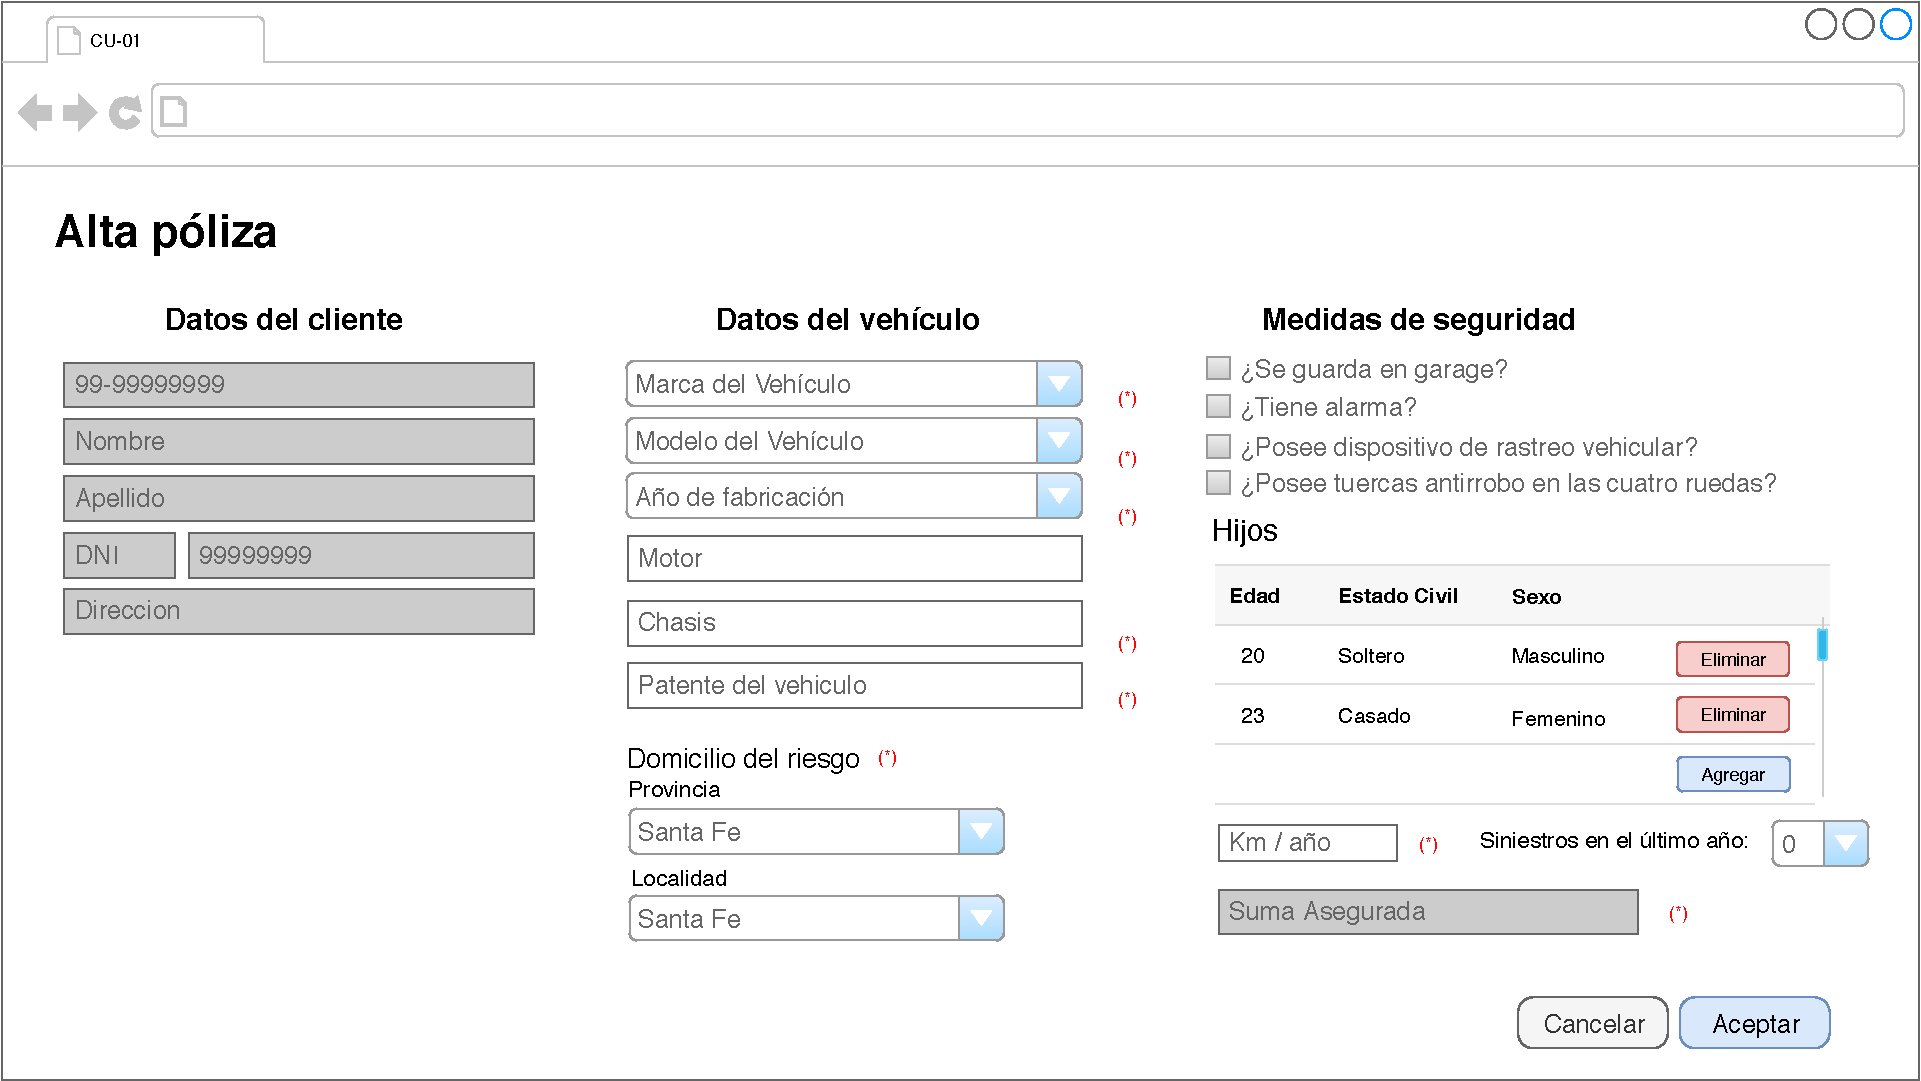
\includegraphics[width=\textwidth]{CU1/CU-011.pdf}
\caption{Caso de uso 1 (flujo principal)}
\end{figure}
\vfill

\vfill
\begin{figure}[h!]
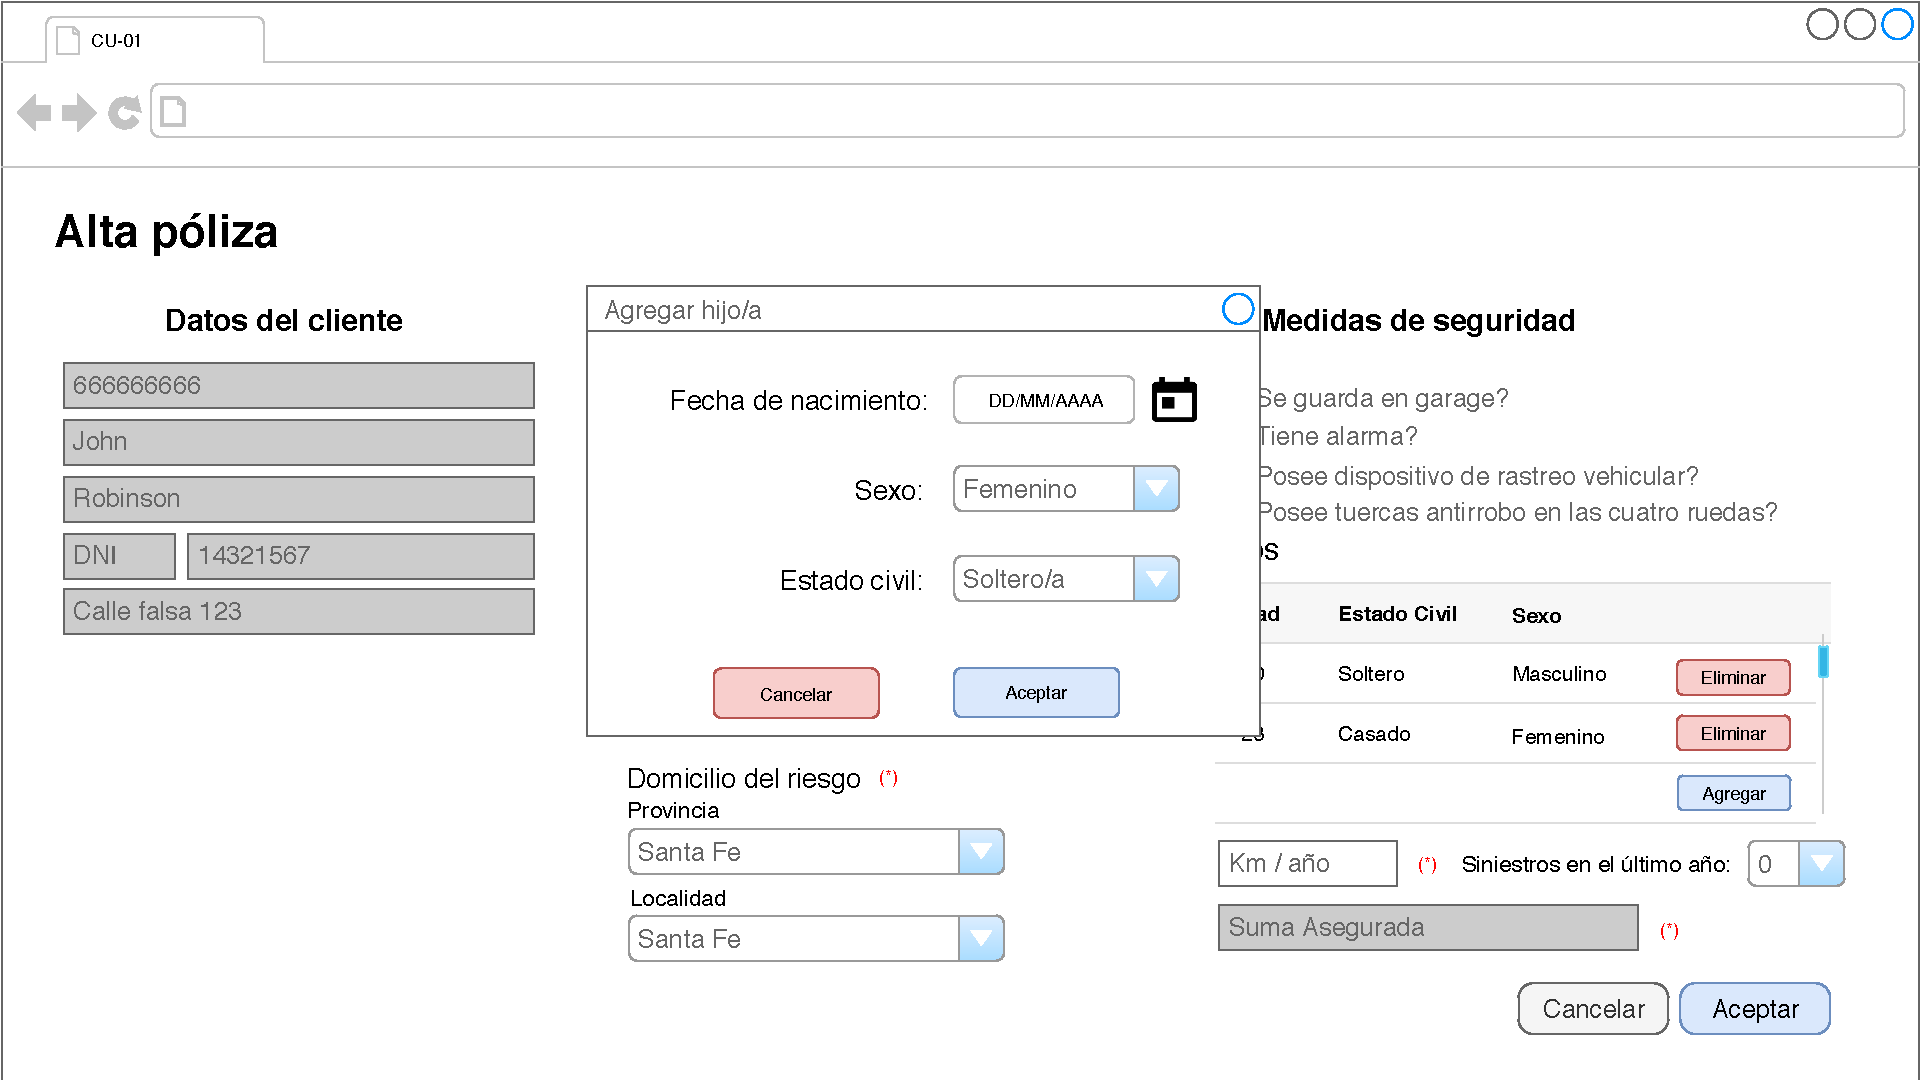
\includegraphics[width=\textwidth]{CU1/CU-012.pdf}
\caption{Caso de uso 1 (flujo principal)}
\end{figure}
\vfill

\vfill
\begin{figure}[h!]
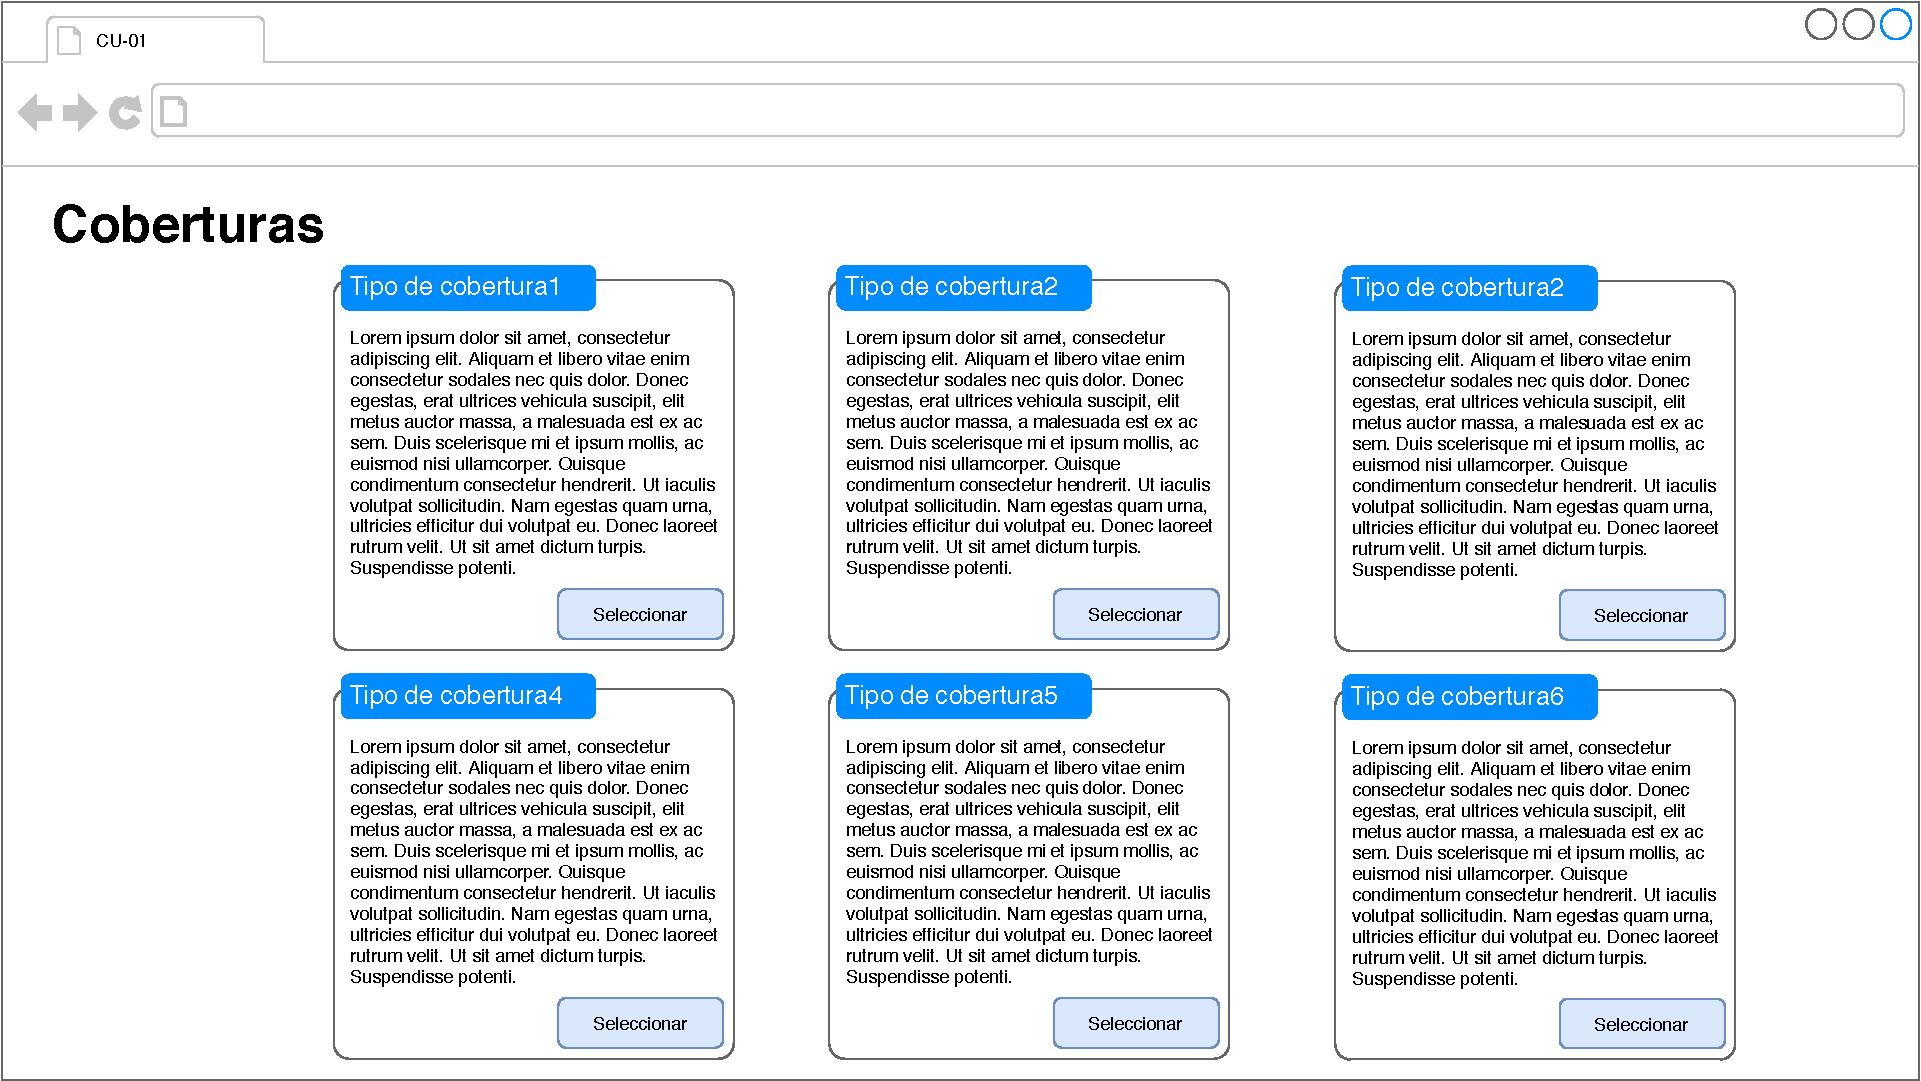
\includegraphics[width=\textwidth]{CU1/CU-013.pdf}
\caption{Caso de uso 1 (flujo principal)}
\end{figure}
\vfill

\vfill
\begin{figure}[h!]
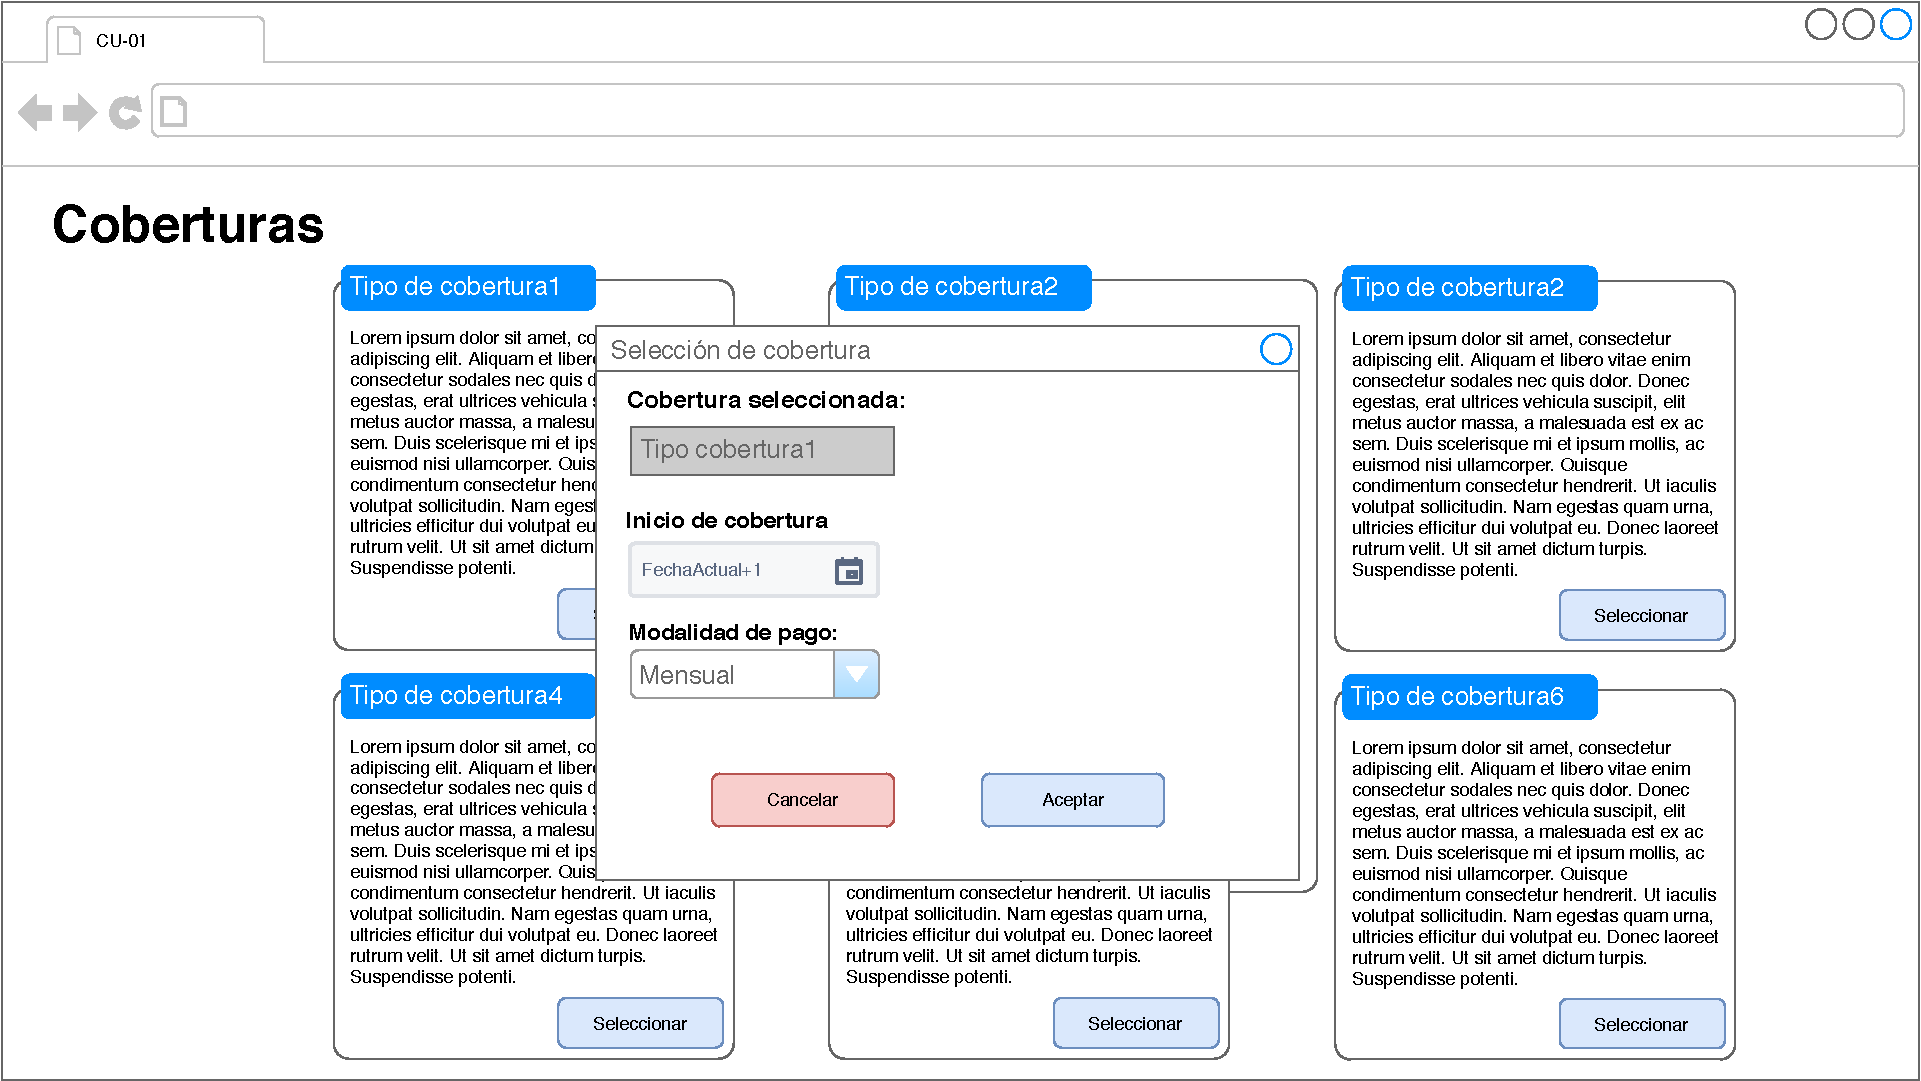
\includegraphics[width=\textwidth]{CU1/CU-014.pdf}
\caption{Caso de uso 1 (flujo principal)}
\end{figure}
\vfill

\vfill
\begin{figure}[h!]
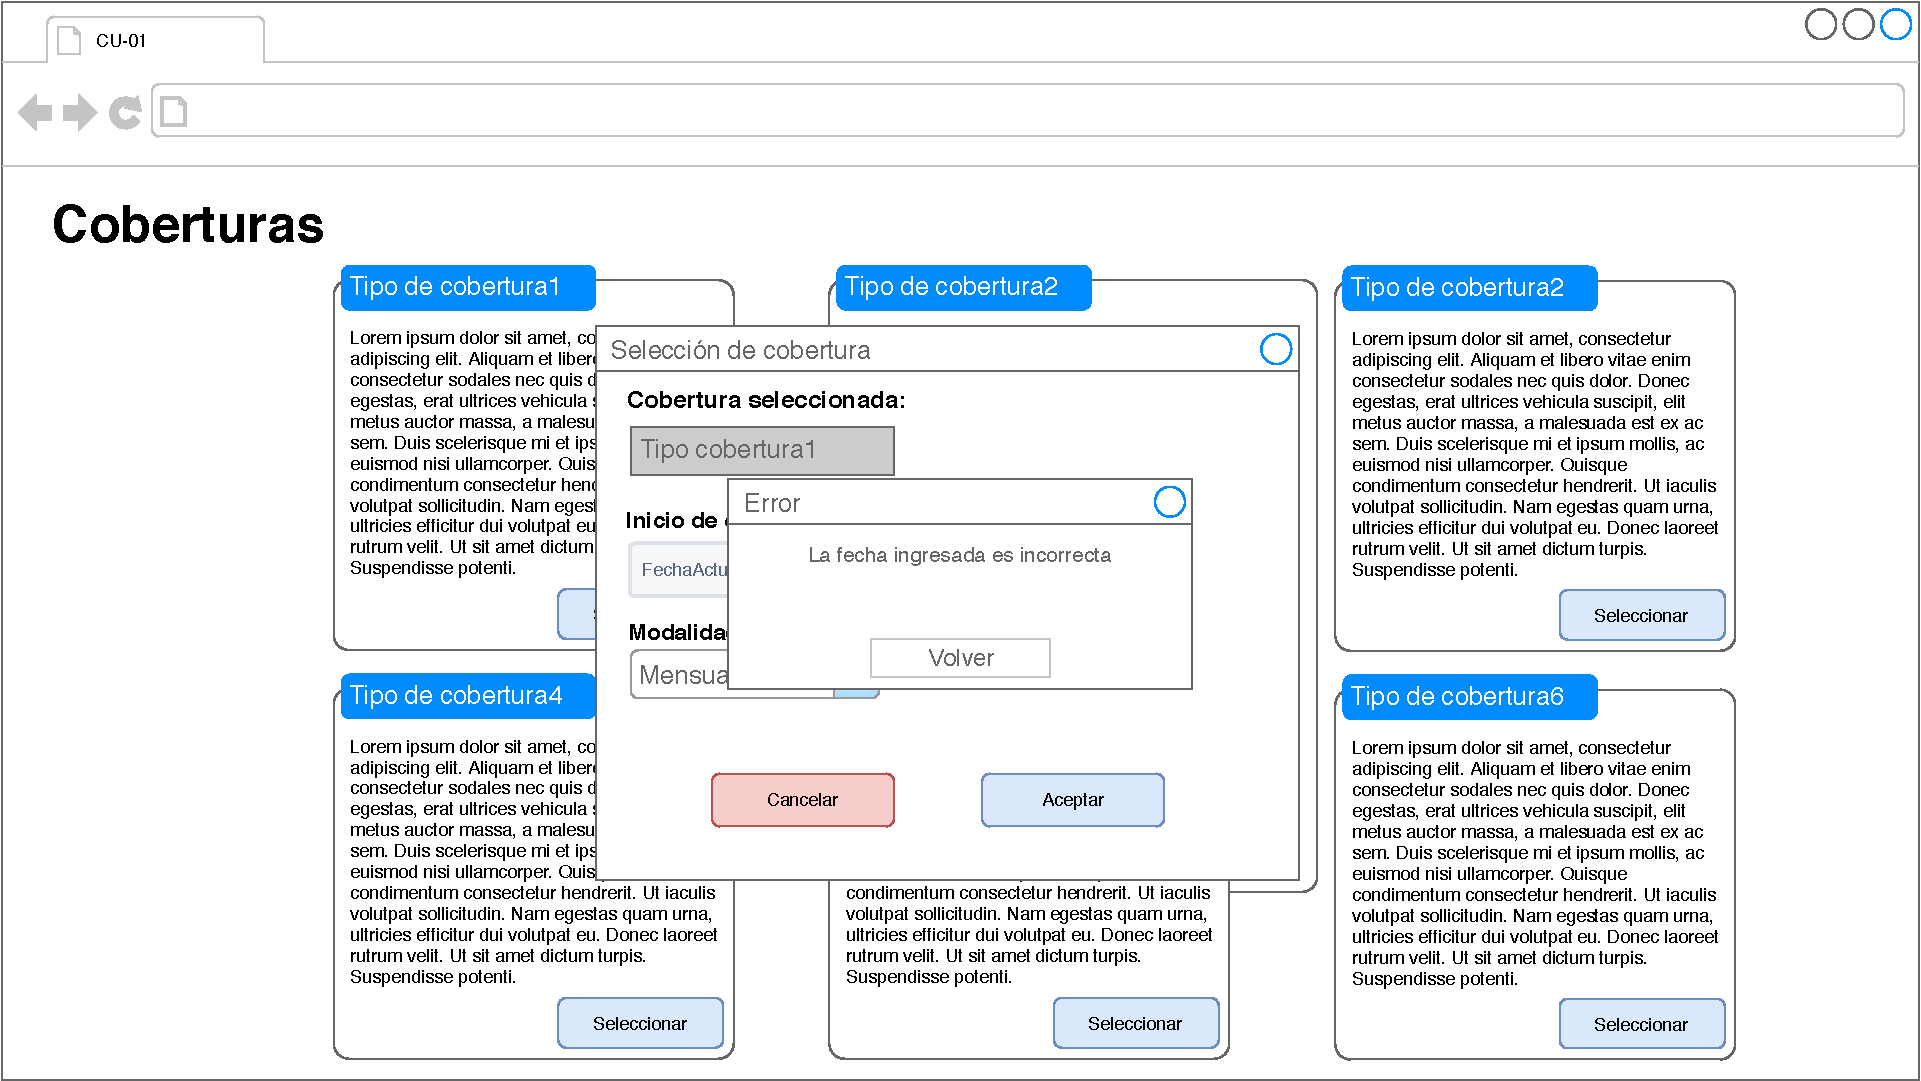
\includegraphics[width=\textwidth]{CU1/CU-015.pdf}
\caption{Caso de uso 1 (error de entrada)}
\end{figure}
\vfill

\vfill
\begin{figure}[h!]
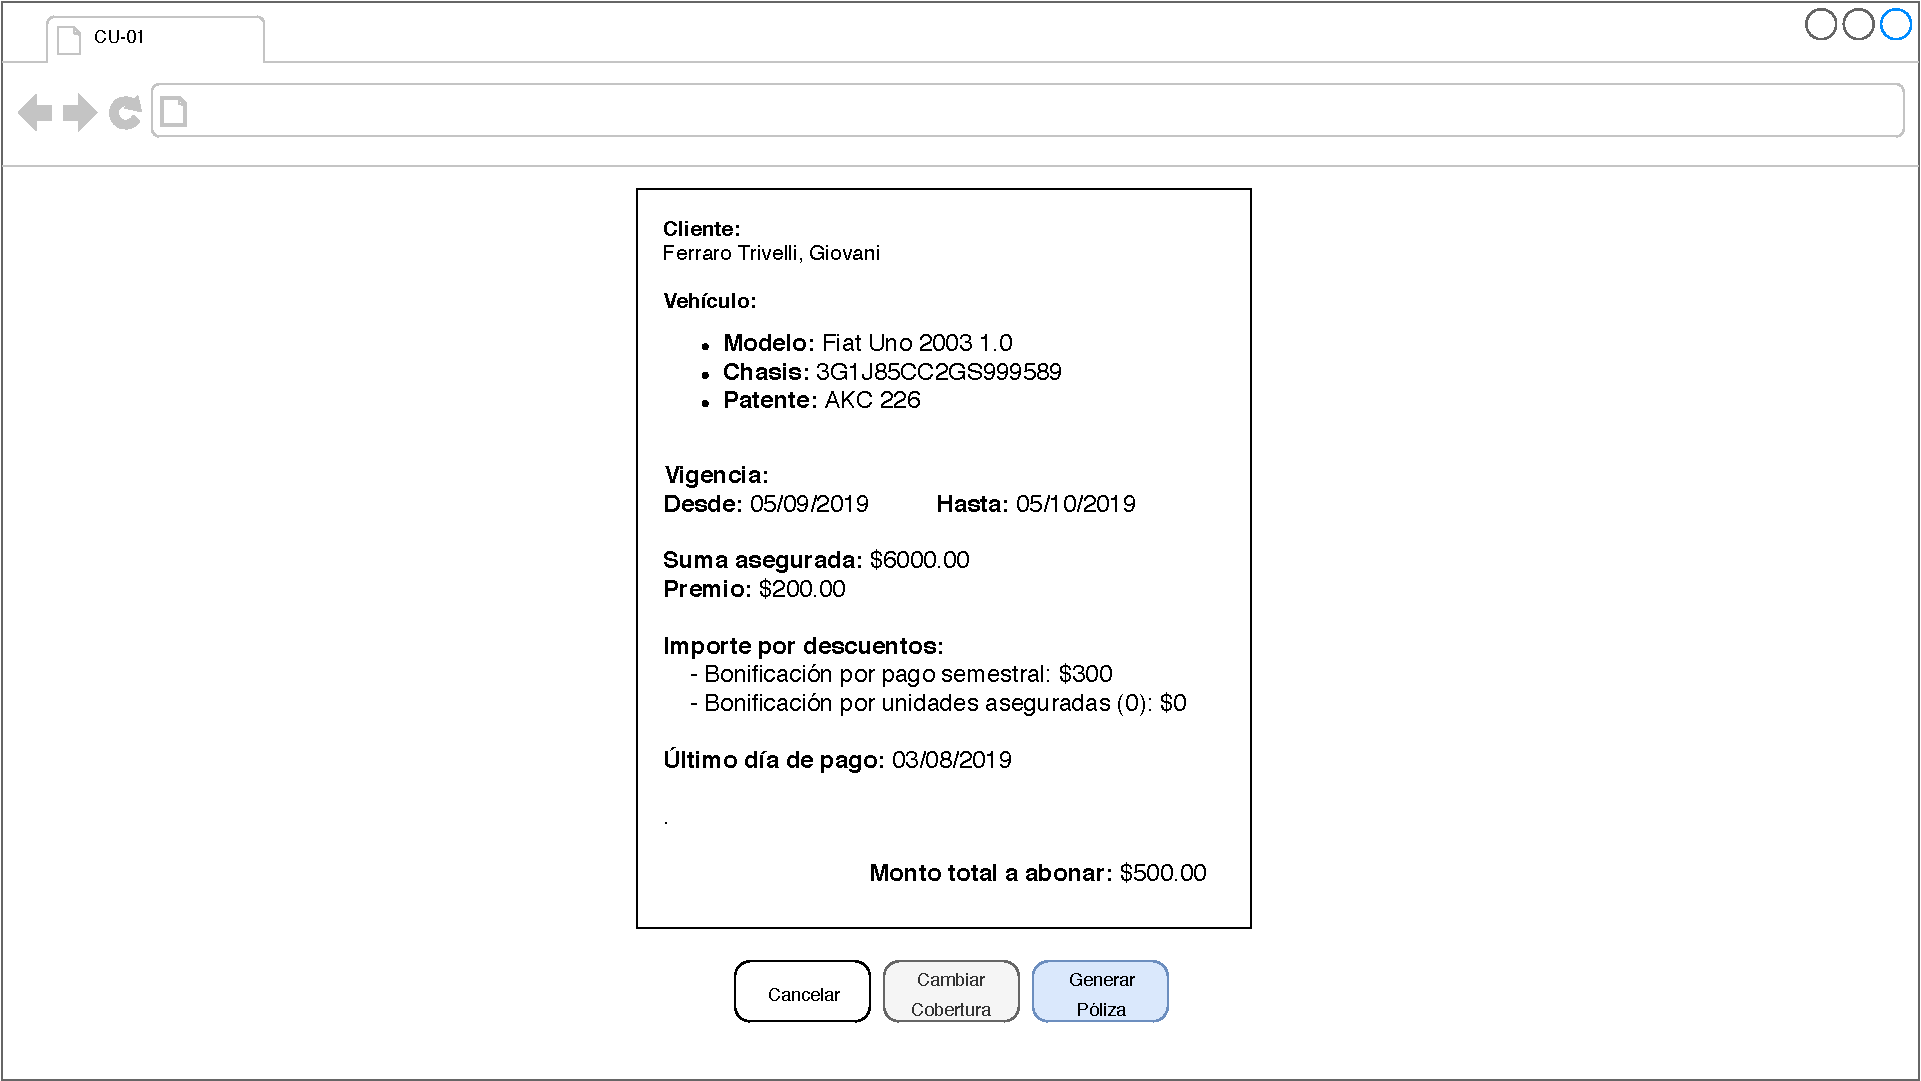
\includegraphics[width=\textwidth]{CU1/CU-016.pdf}
\caption{Caso de uso 1 (flujo principal)}
\end{figure}
\vfill

\vfill
\begin{figure}[h!]
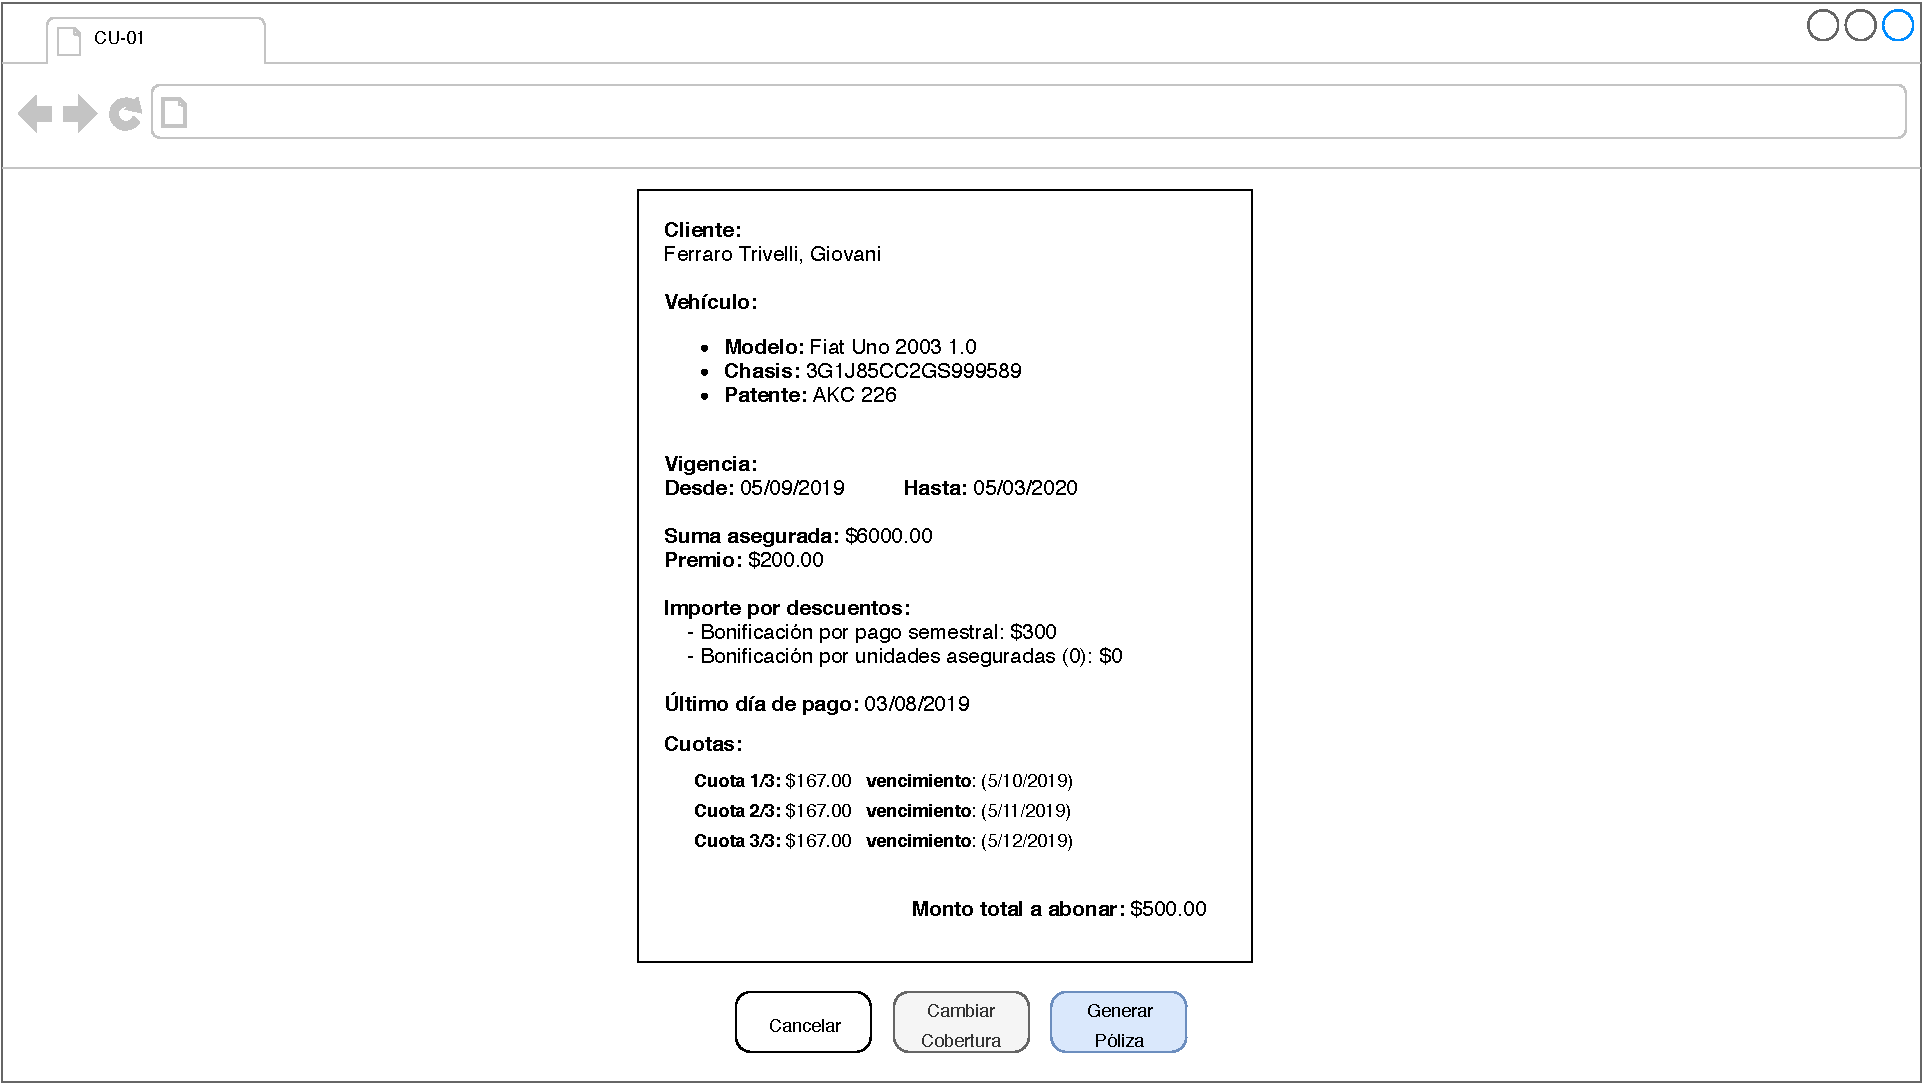
\includegraphics[width=\textwidth]{CU1/CU-017.pdf}
\caption{Caso de uso 1 (flujo principal)}
\end{figure}
\vfill

%%%%%%%%%%%%%%%%%%%%%%%
%%%%%%        CASO DE USO 2         %%%%%
%%%%%%%%%%%%%%%%%%%%%%%
\vfill
\begin{figure}[h!]
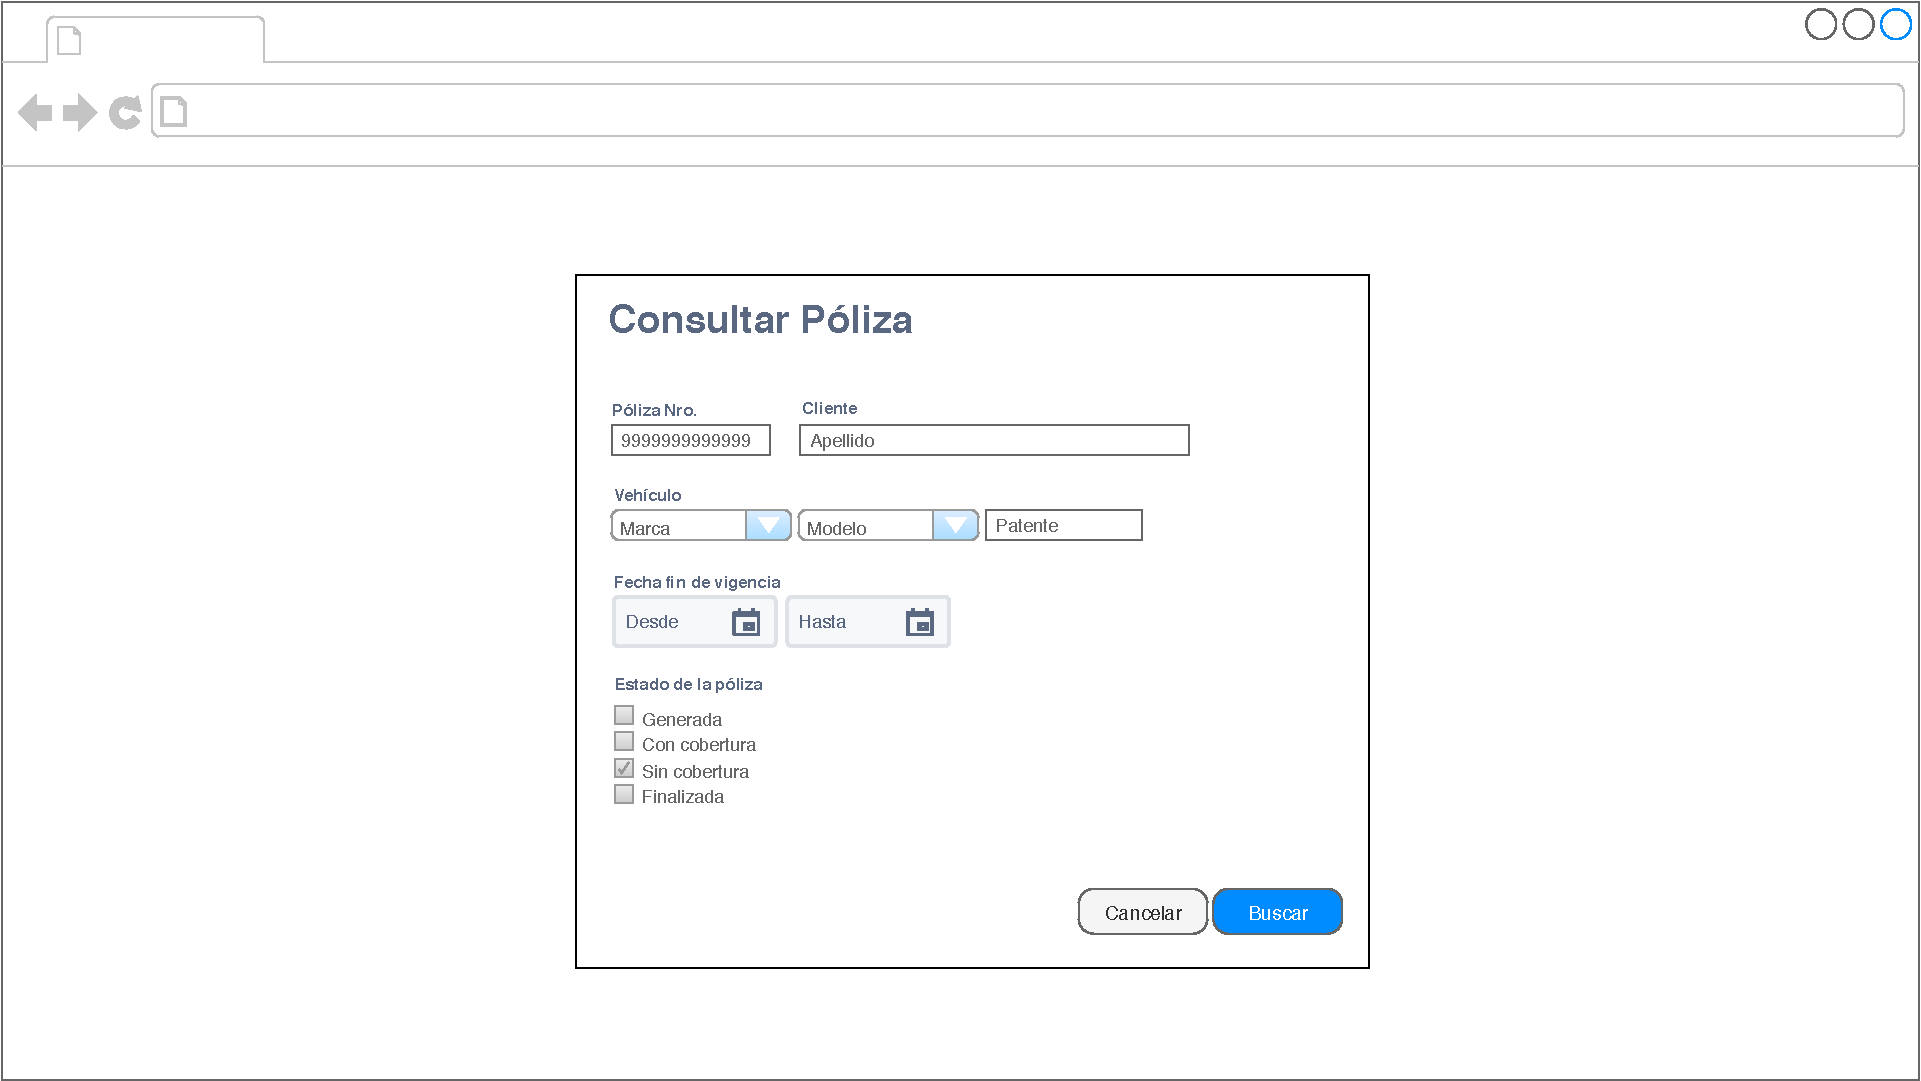
\includegraphics[width=\textwidth]{CU2/CU-021.pdf}
\caption{Caso de uso 2 (flujo principal)}
\end{figure}
\vfill

\vfill
\begin{figure}[h!]
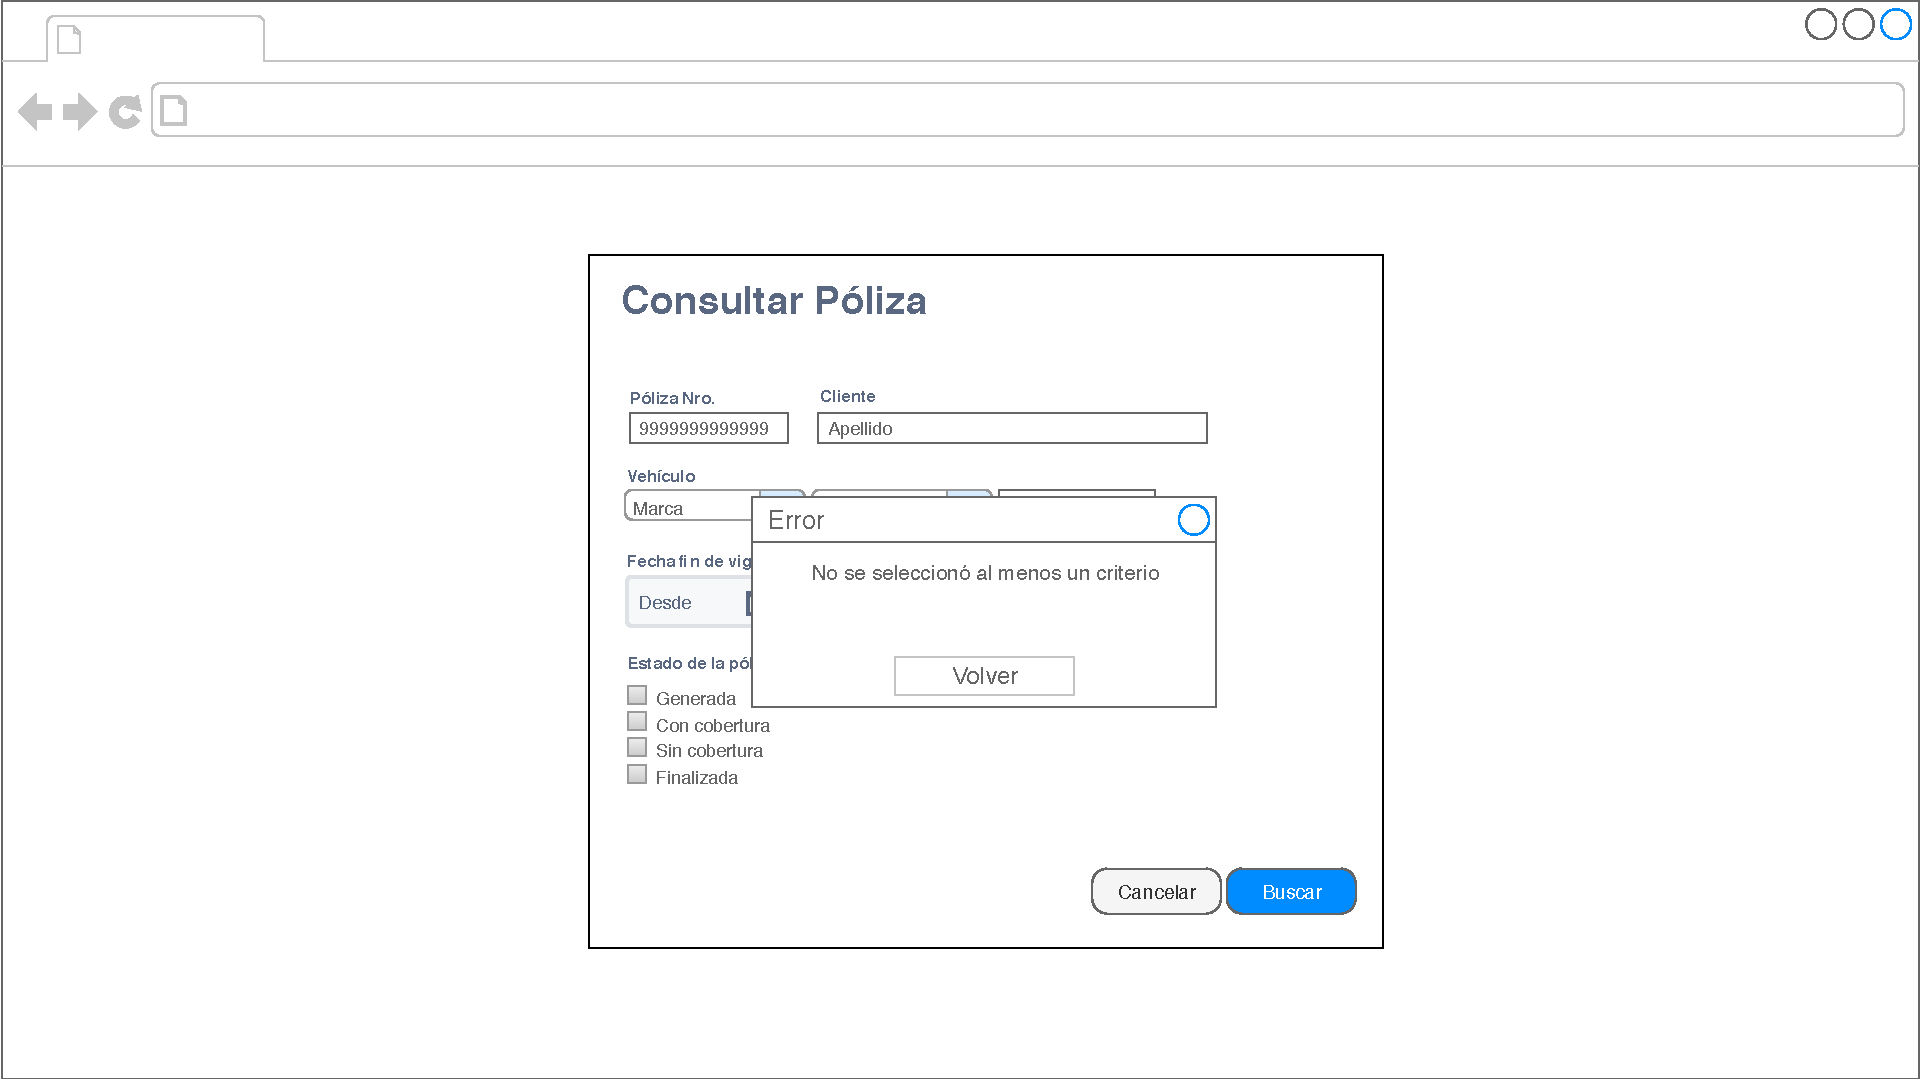
\includegraphics[width=\textwidth]{CU2/CU-022.pdf}
\caption{Caso de uso 2 (error de entrada)}
\end{figure}
\vfill

\vfill
\begin{figure}[h!]
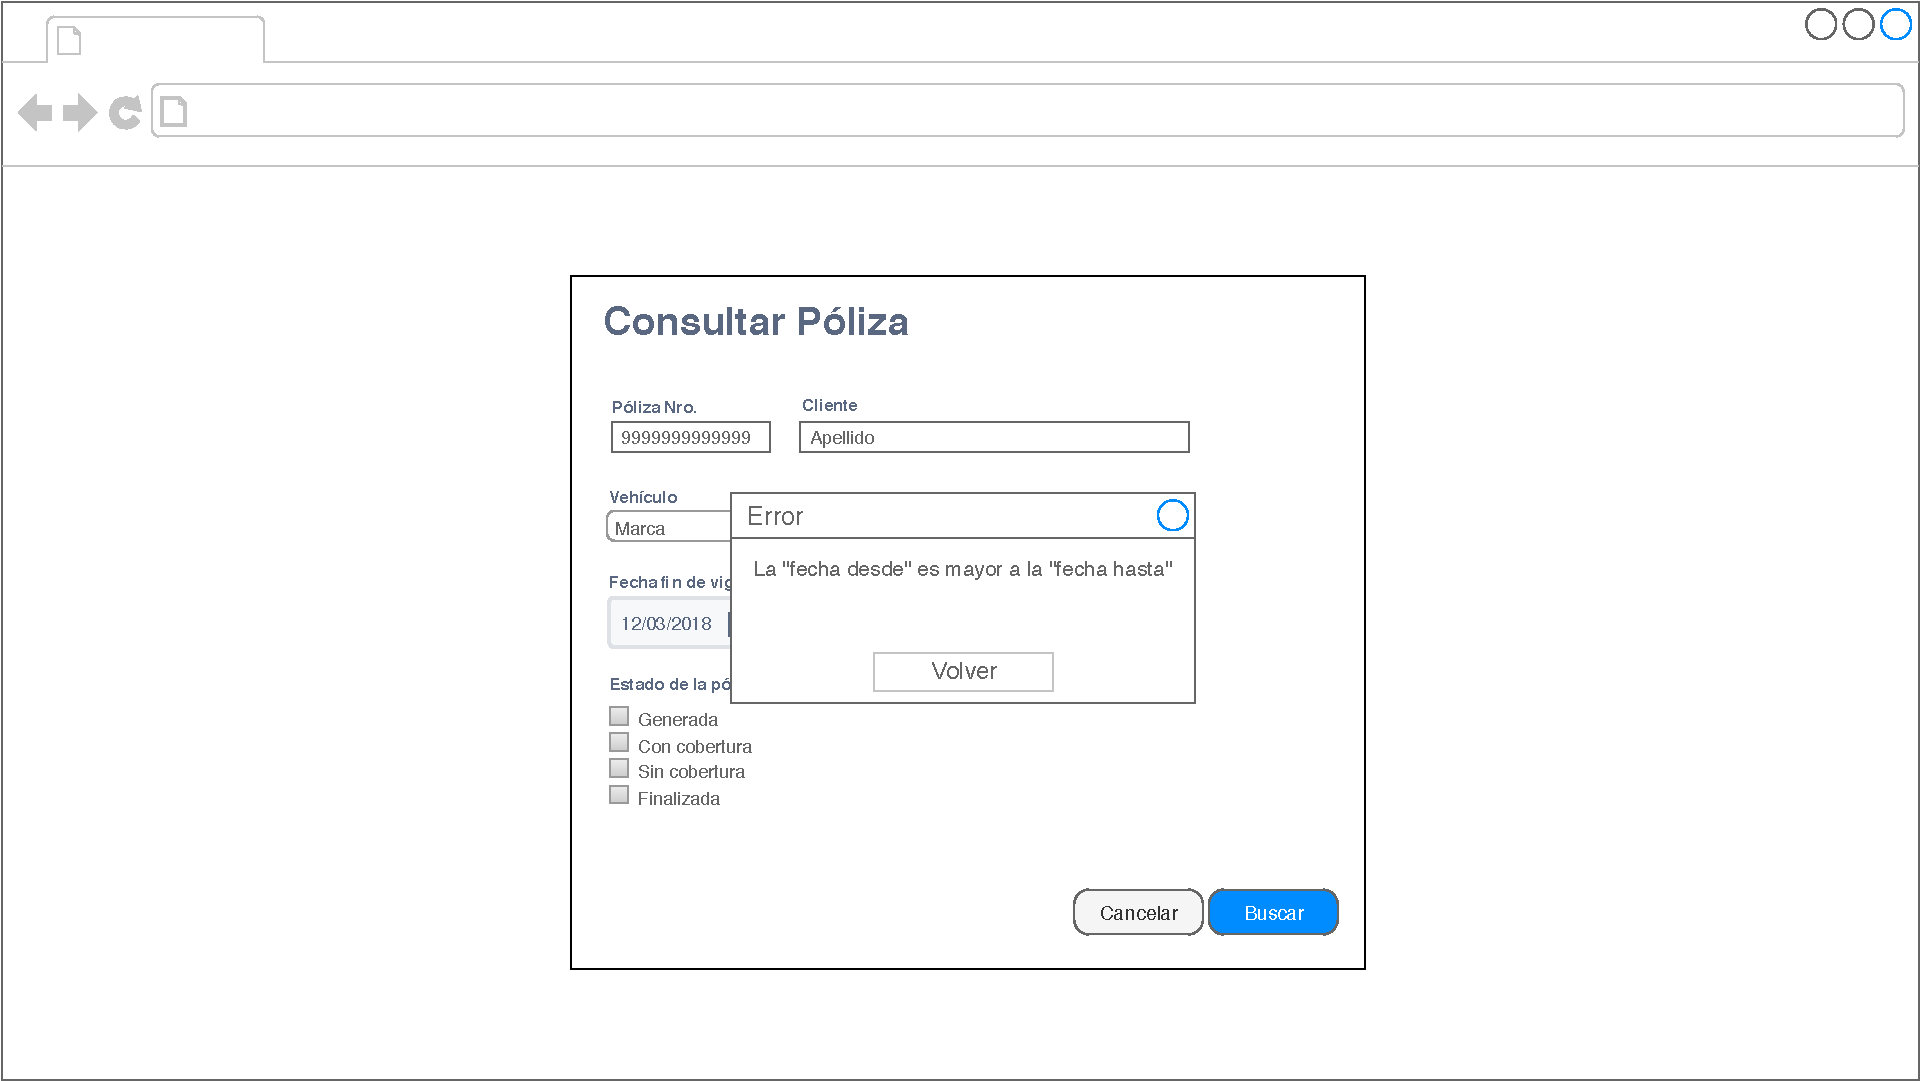
\includegraphics[width=\textwidth]{CU2/CU-023.pdf}
\caption{Caso de uso 2 (error de entrada)}
\end{figure}
\vfill

\vfill
\begin{figure}[h!]
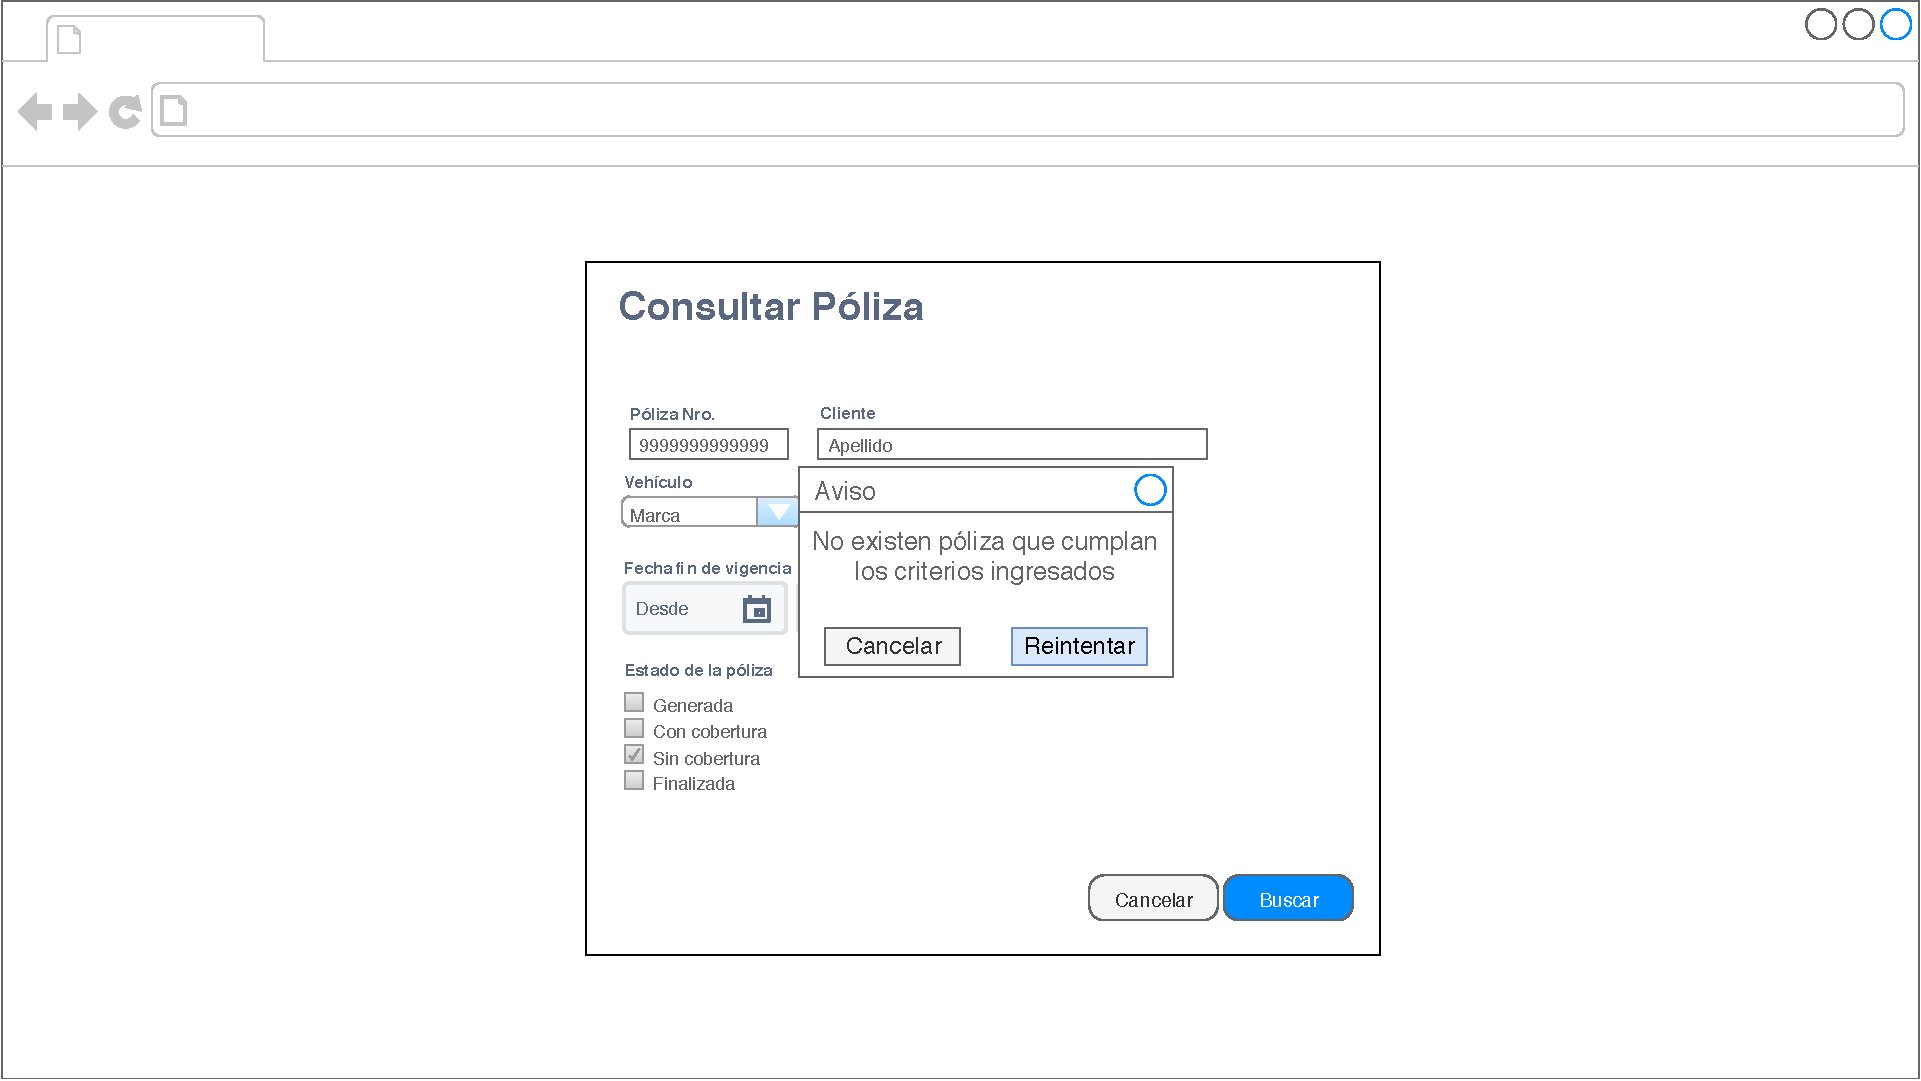
\includegraphics[width=\textwidth]{CU2/CU-025.pdf}
\caption{Caso de uso 2 (no se encuentran registros)}
\end{figure}
\vfill


\vfill
\begin{figure}[h!]
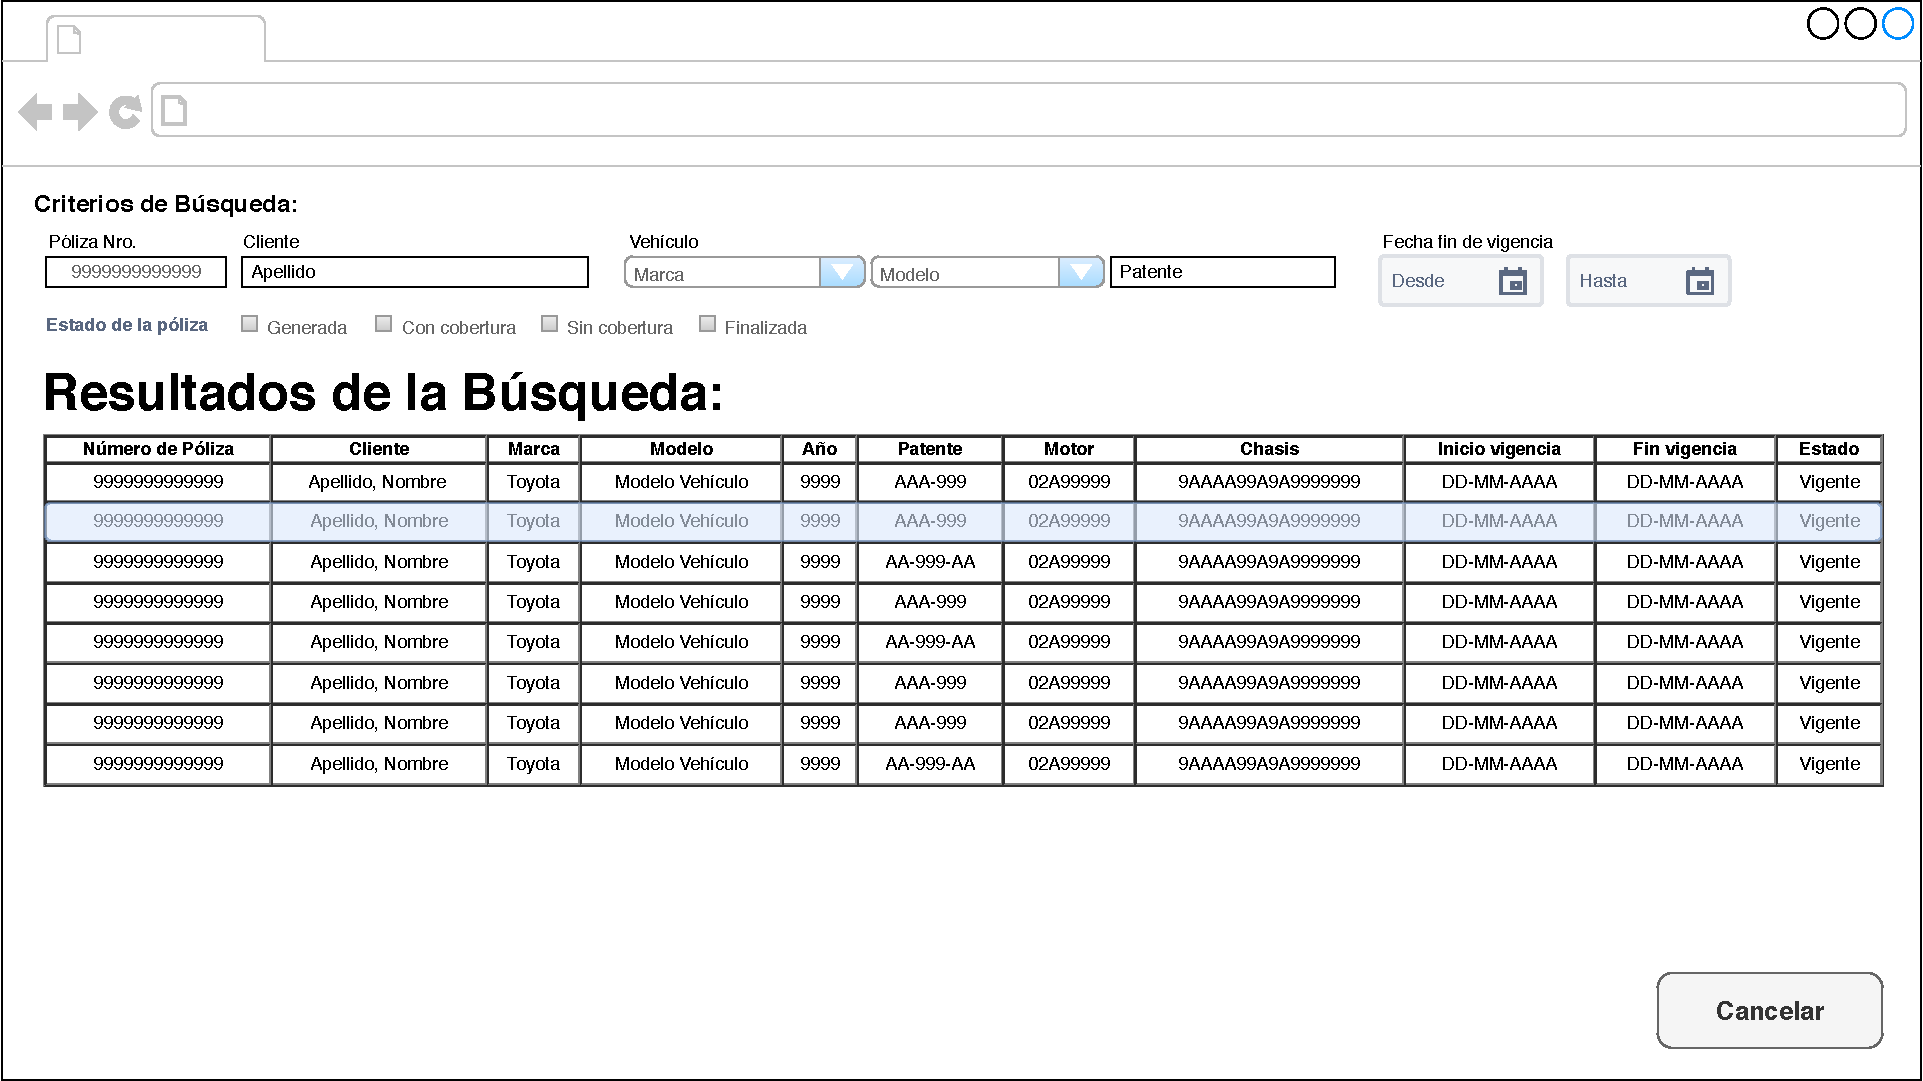
\includegraphics[width=\textwidth]{CU2/CU-024.pdf}
\caption{Caso de uso 2 (flujo principal)}
\end{figure}
\vfill


\vfill
\begin{figure}[h!]
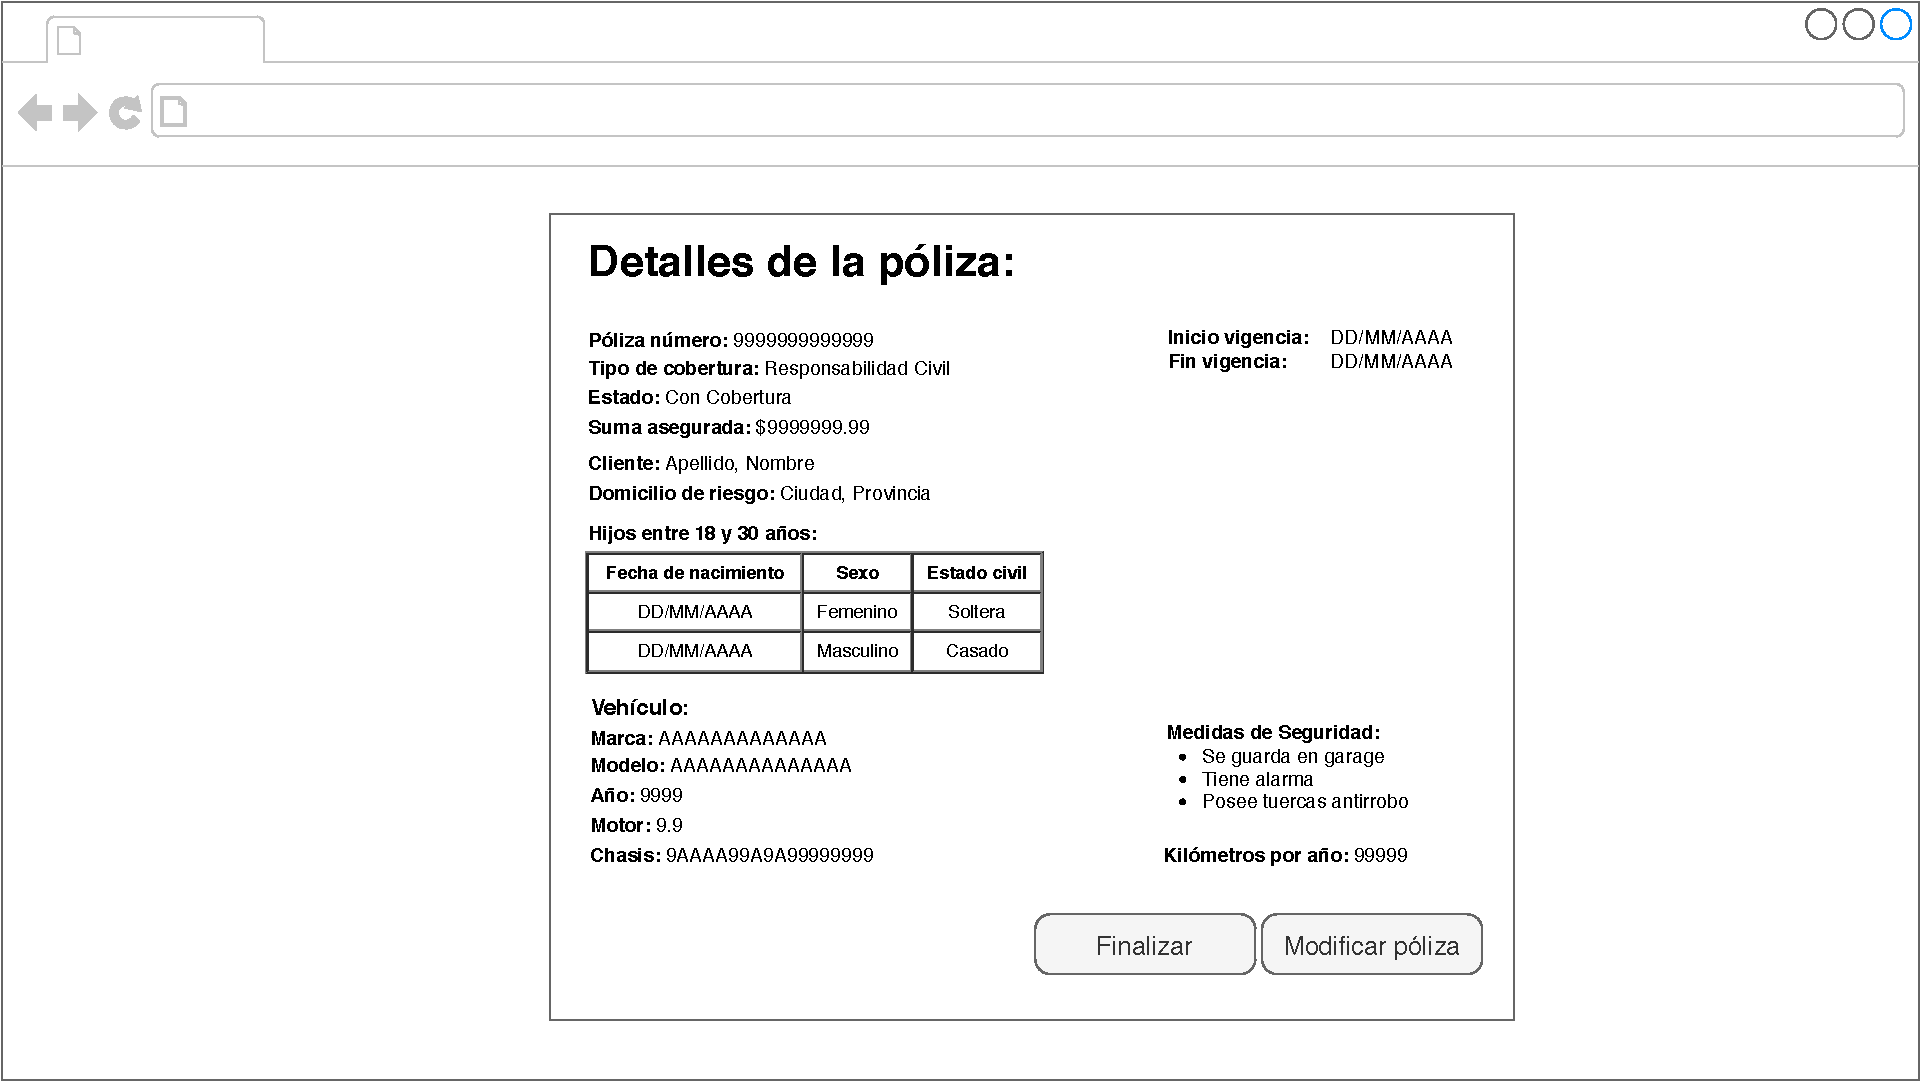
\includegraphics[width=\textwidth]{CU2/CU-026.pdf}
\caption{Caso de uso 2 (flujo principal)}
\end{figure}
\vfill



%%%%%%%%%%%%%%%%%%%%%%%
%%%%%%        CASO DE USO 3         %%%%%
%%%%%%%%%%%%%%%%%%%%%%%


\vfill
\begin{figure}[h!]
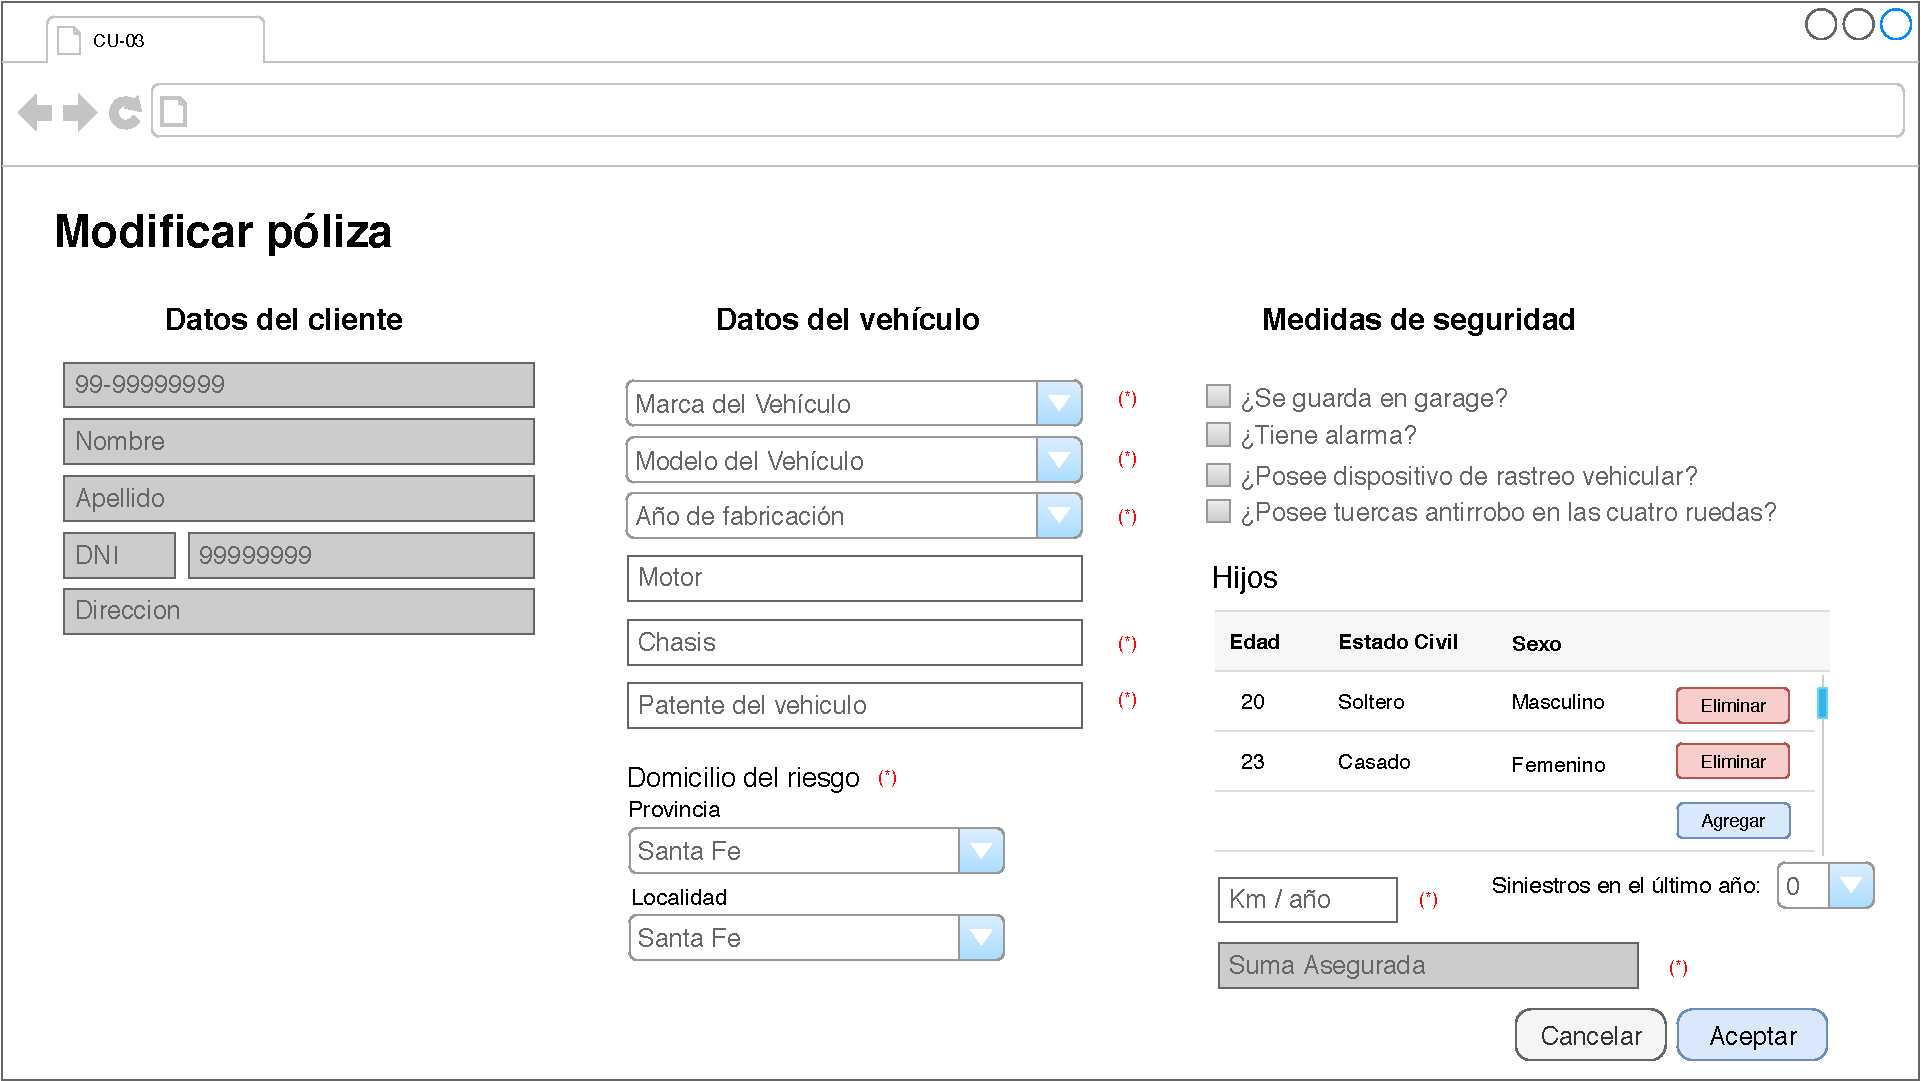
\includegraphics[width=\textwidth]{CU3/CU-031.pdf}
\caption{Caso de uso 3 (flujo principal)}
\end{figure}
\vfill



\vfill
\begin{figure}[h!]
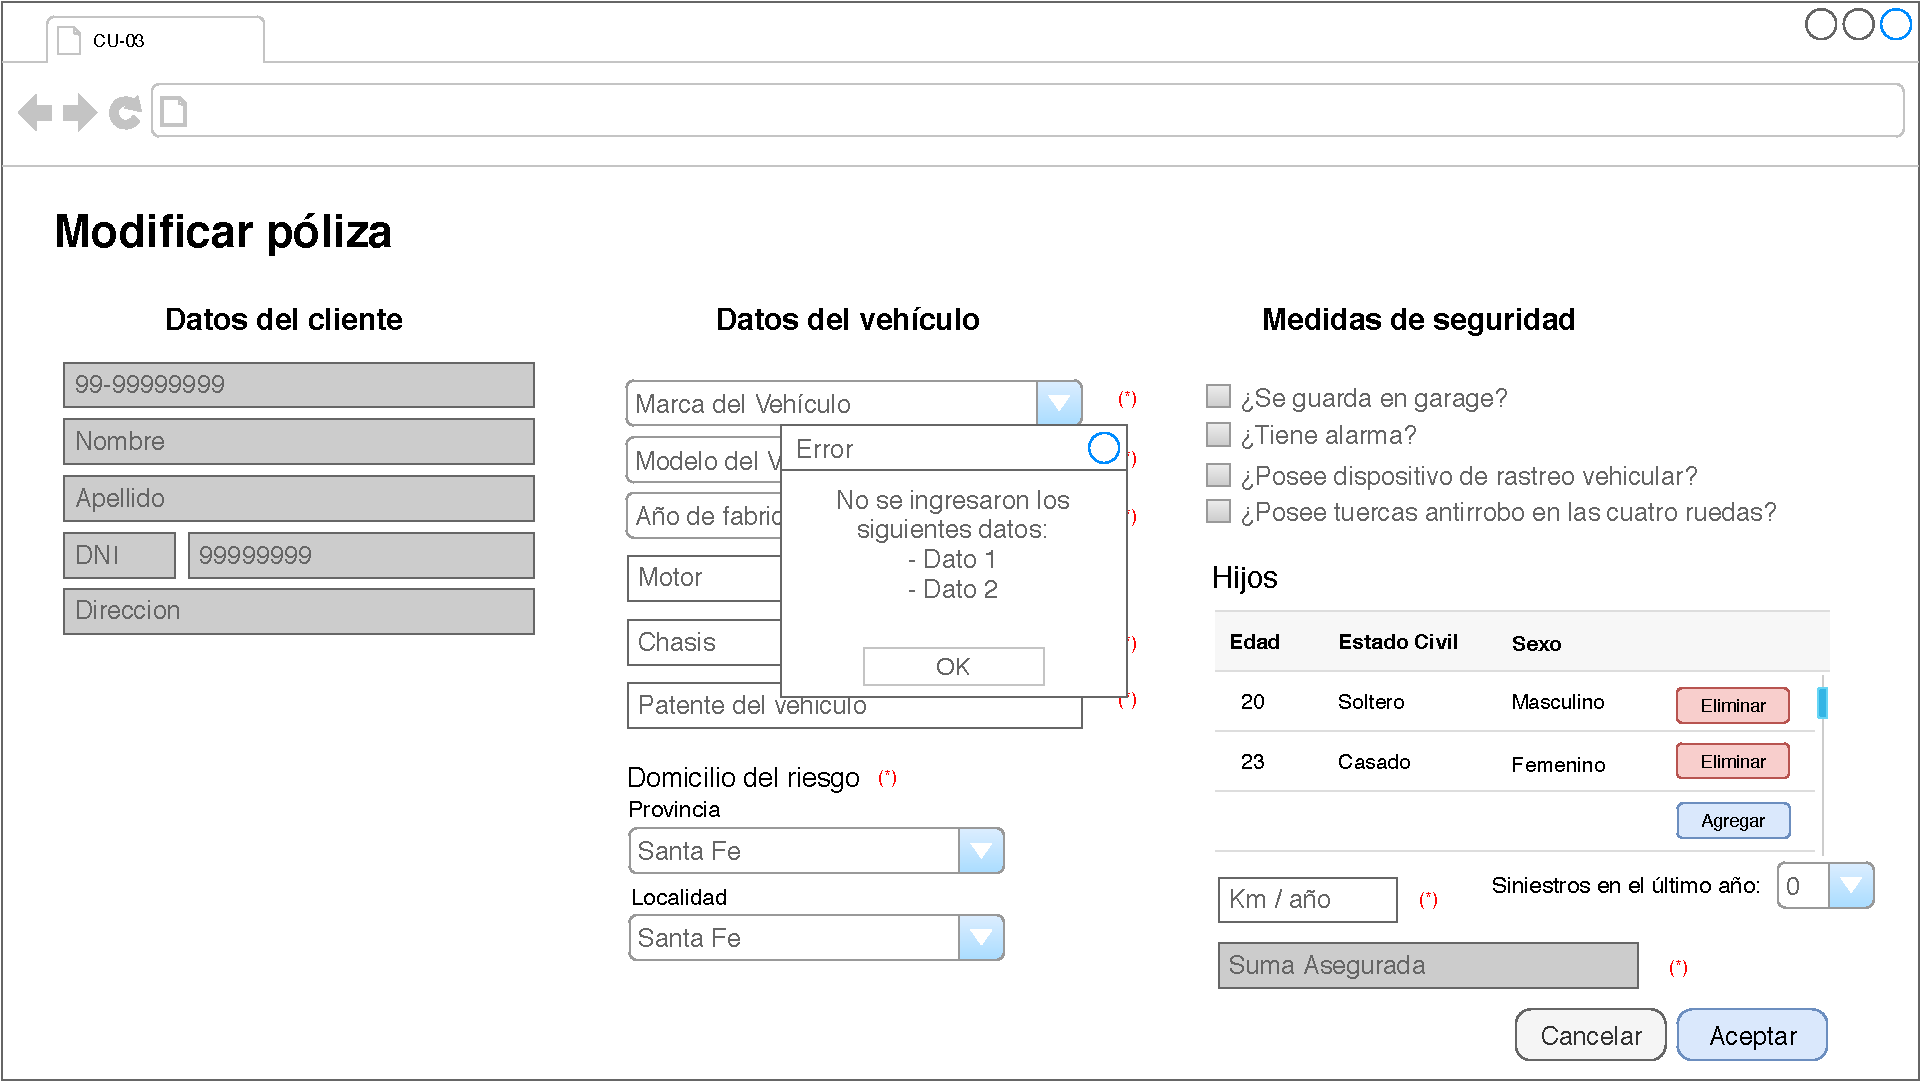
\includegraphics[width=\textwidth]{CU3/CU-032.pdf}
\caption{Caso de uso 3 (error de entrada)}
\end{figure}
\vfill

\vfill
\begin{figure}[h!]
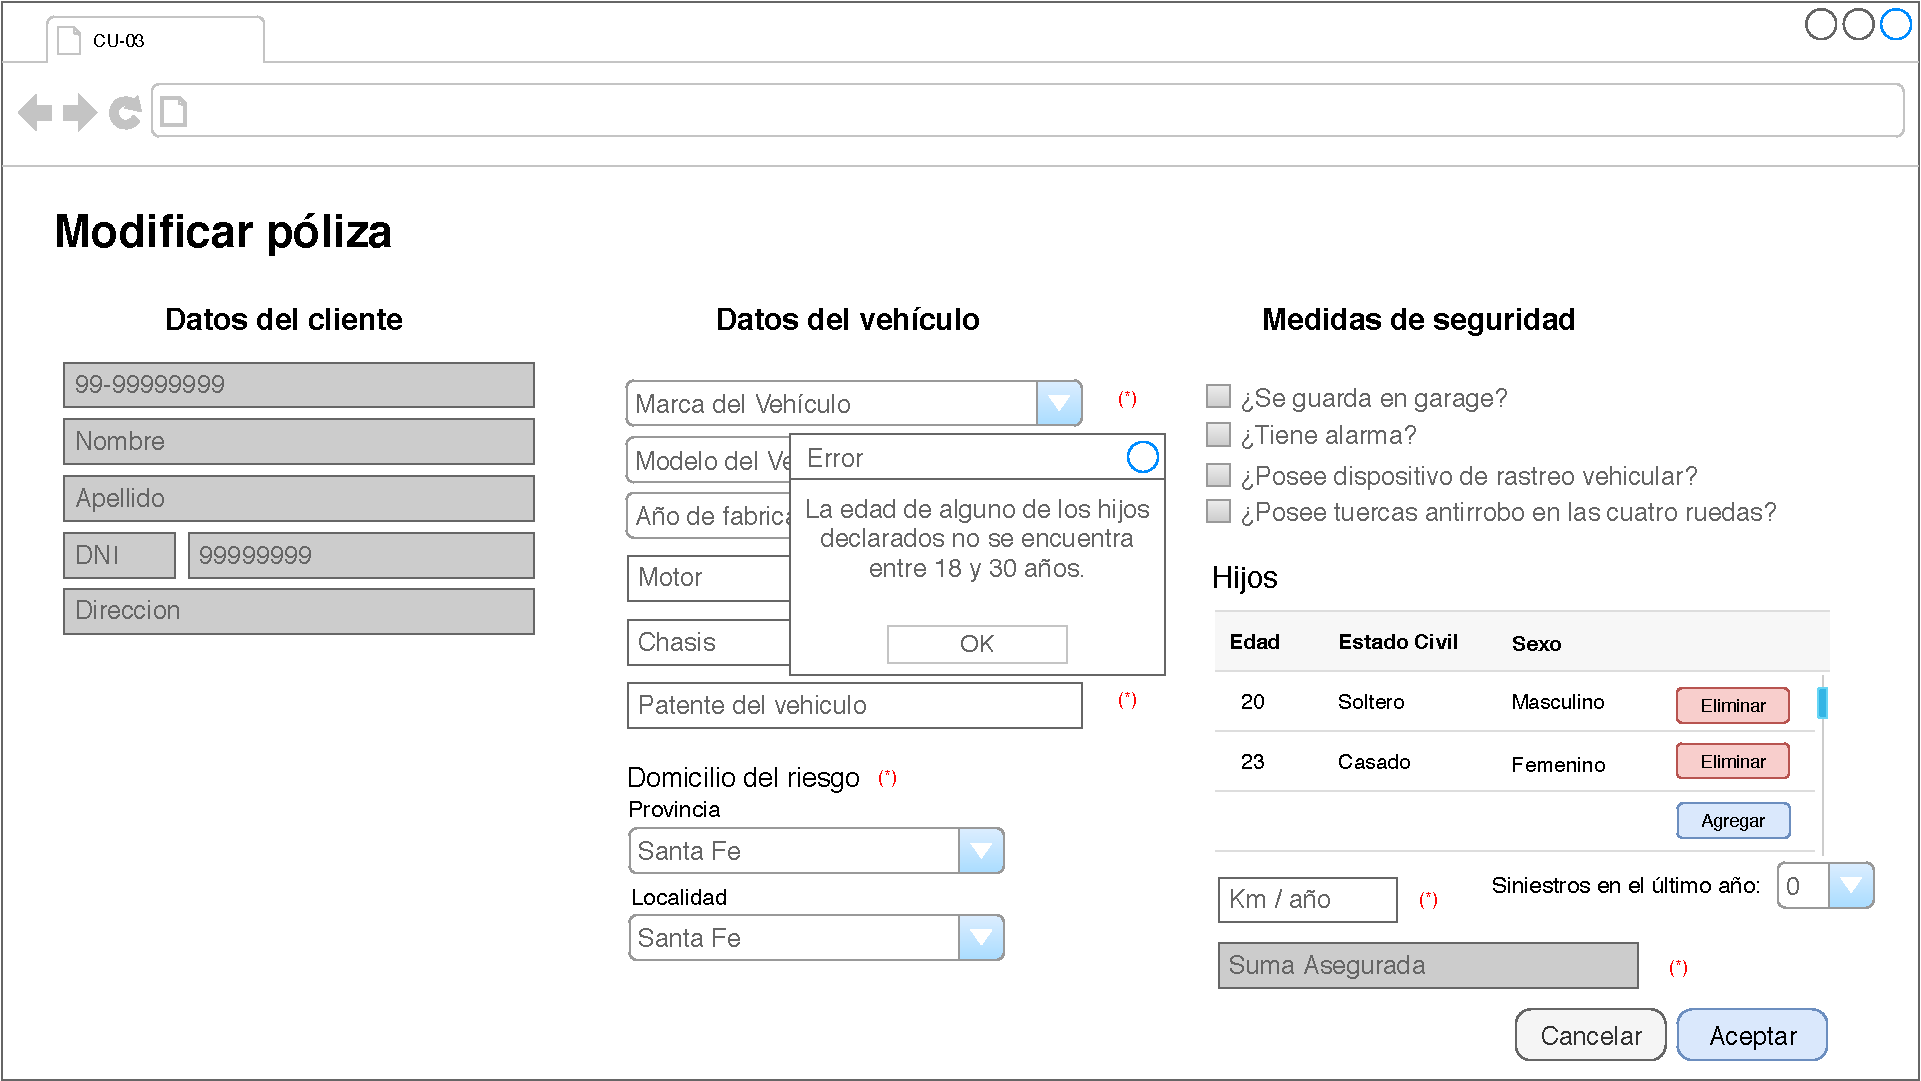
\includegraphics[width=\textwidth]{CU3/CU-033.pdf}
\caption{Caso de uso 3 (error de entrada)}
\end{figure}
\vfill

\vfill
\begin{figure}[h!]
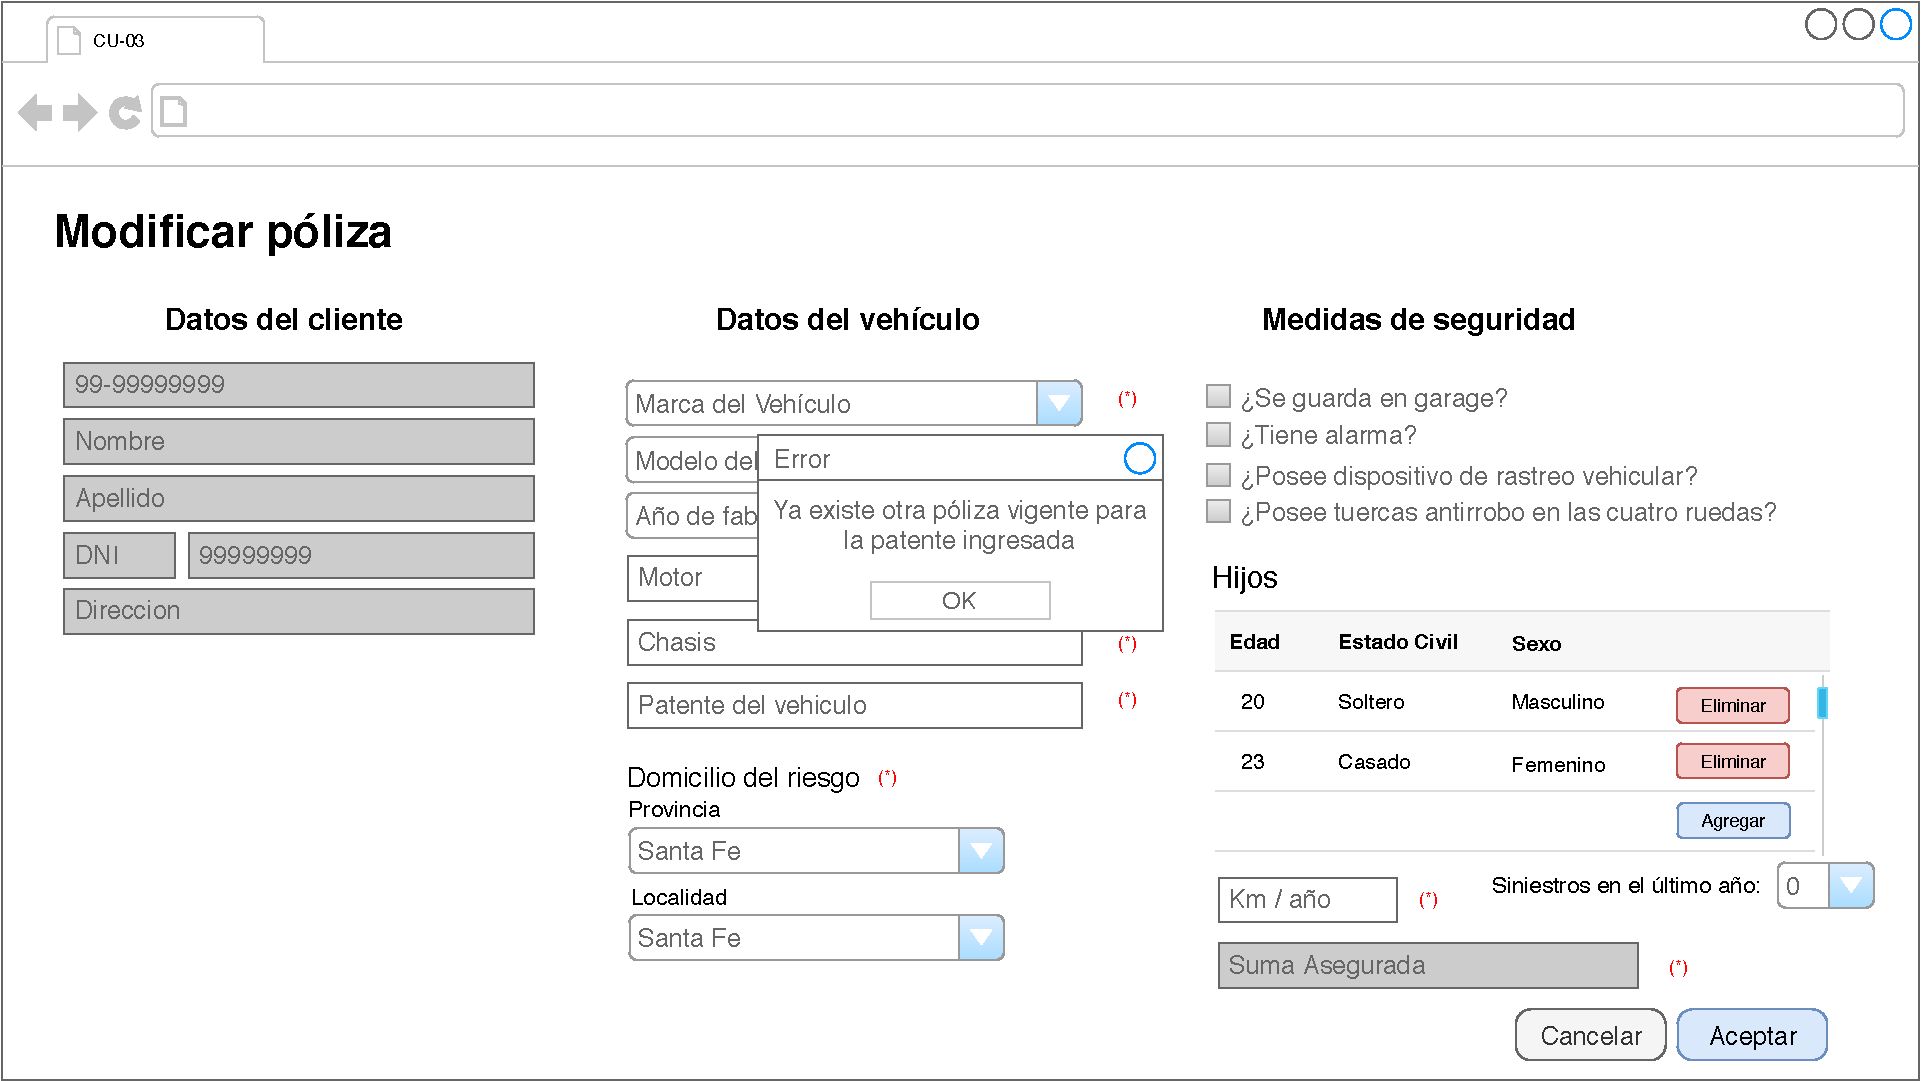
\includegraphics[width=\textwidth]{CU3/CU-034.pdf}
\caption{Caso de uso 3 (ya existe una póliza vigente)}
\end{figure}
\vfill



%%%%%%%%%%%%%%%%%%%%%%%
%%%%%%        CASO DE USO 11         %%%%%
%%%%%%%%%%%%%%%%%%%%%%%

\vfill
\begin{figure}[h!]
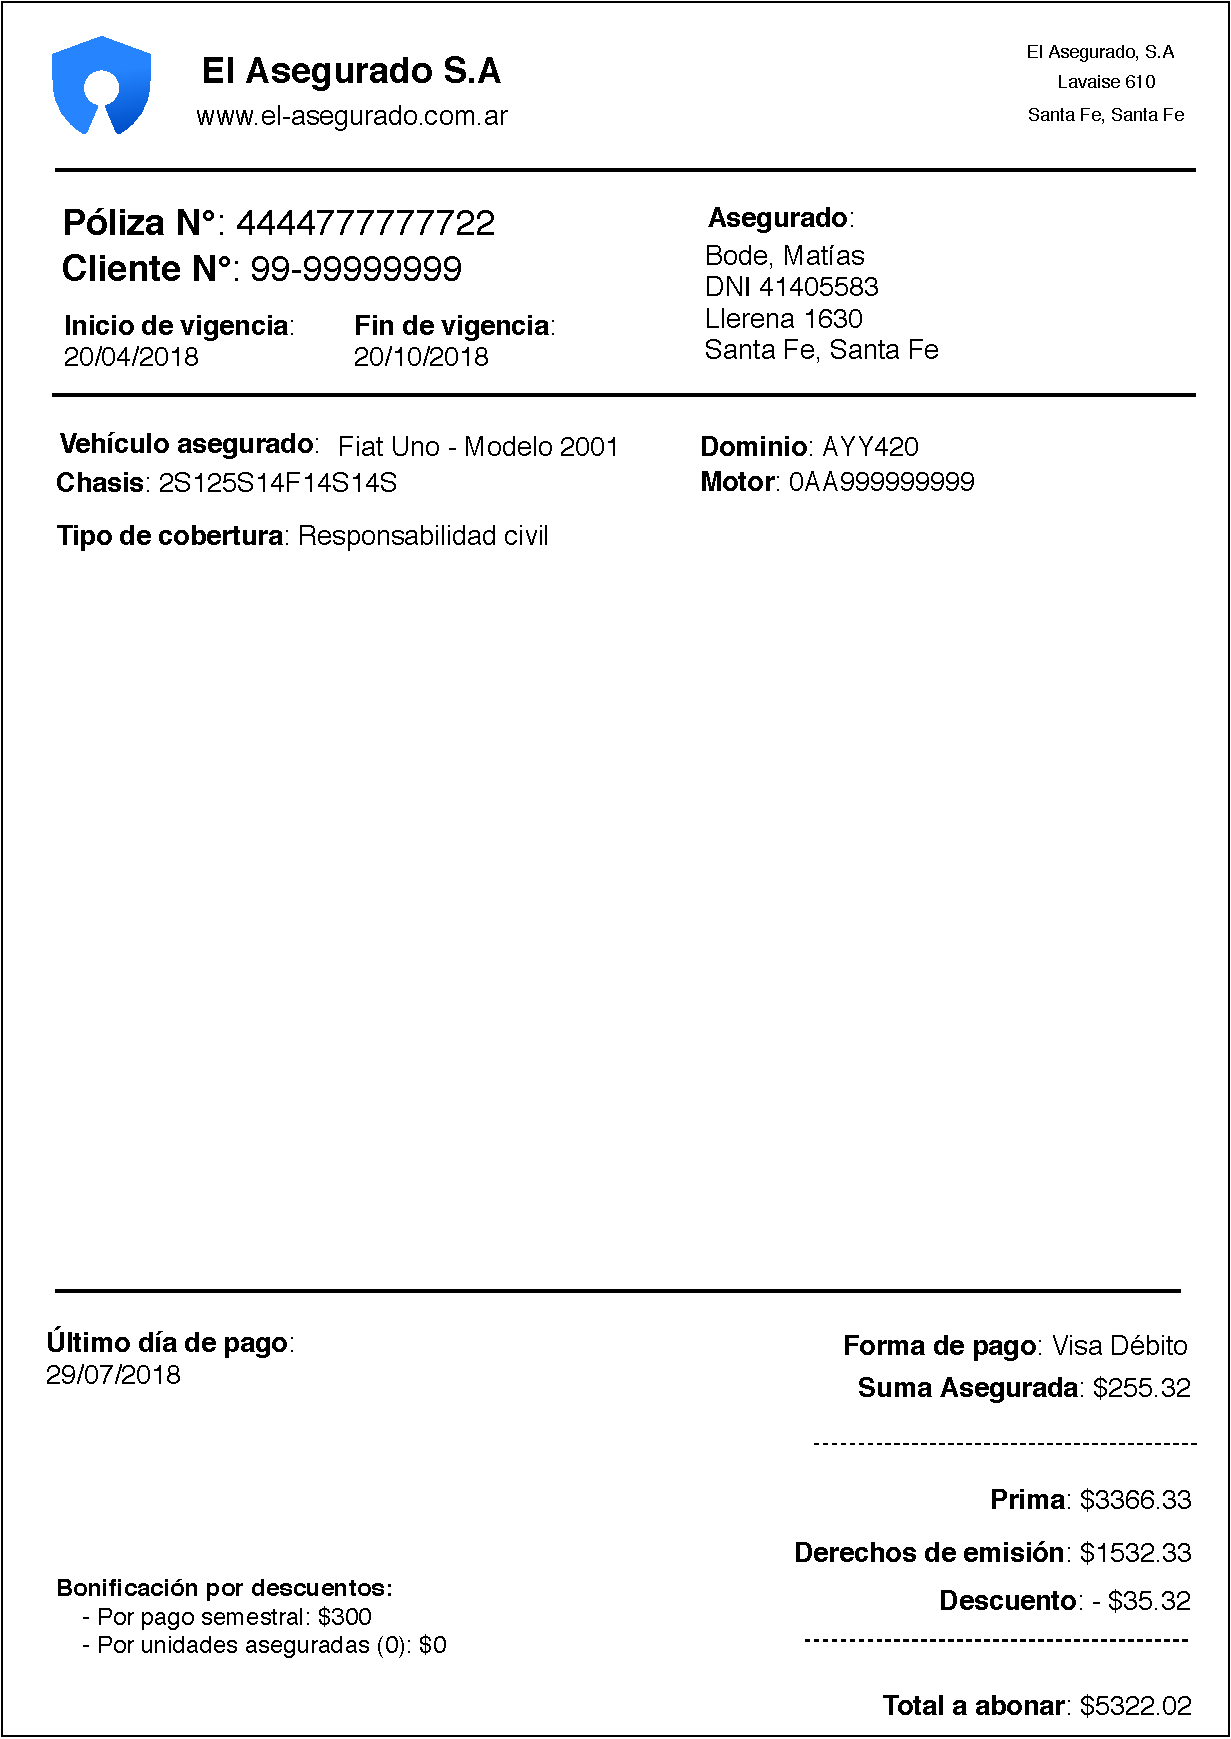
\includegraphics[width=\textwidth]{CU11/CU-111.pdf}
\caption{Caso de uso 11 (flujo principal)}
\end{figure}
\vfill


\vfill
\begin{figure}[h!]
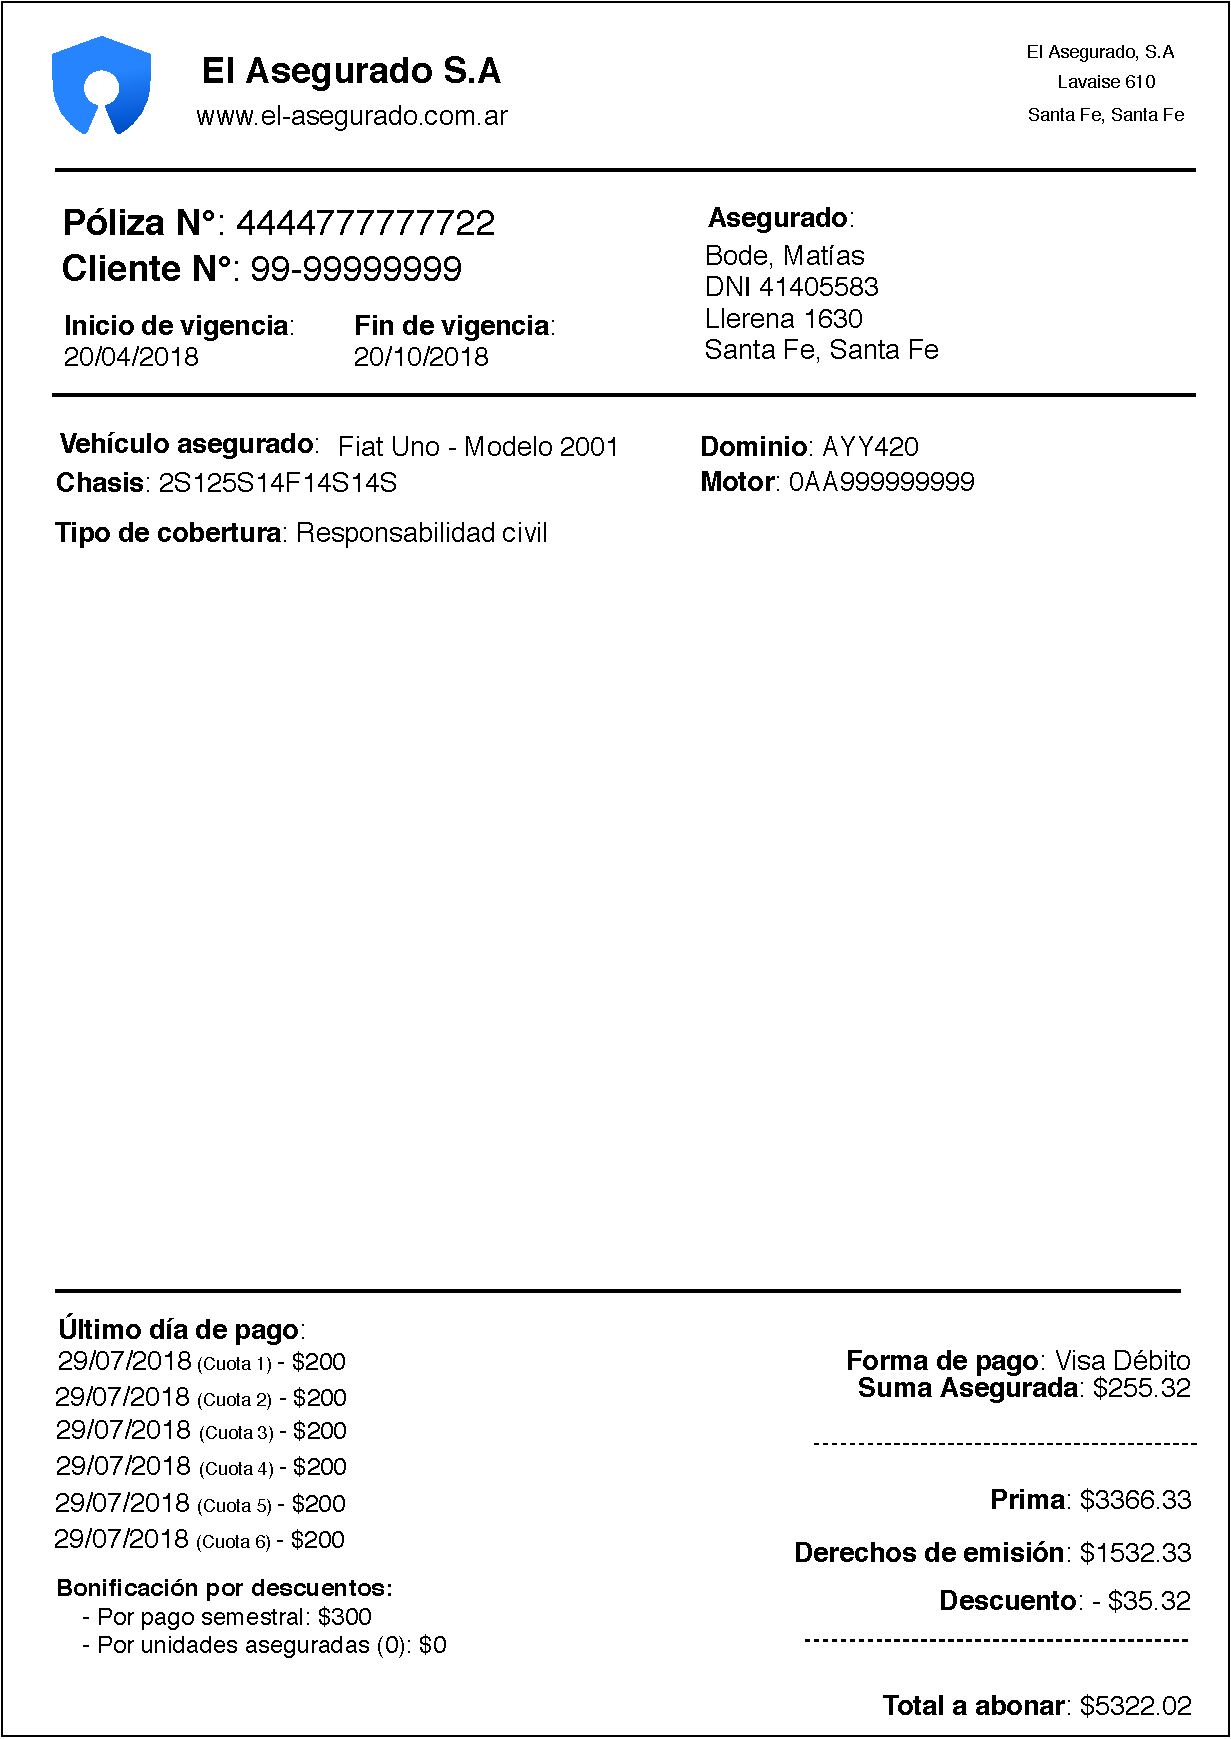
\includegraphics[width=\textwidth]{CU11/CU-112.pdf}
\caption{Caso de uso 11 (flujo principal)}
\end{figure}
\vfill


%%%%%%%%%%%%%%%%%%%%%%%
%%%%%%        CASO DE USO 12         %%%%%
%%%%%%%%%%%%%%%%%%%%%%%
\vfill
\begin{figure}[h!]
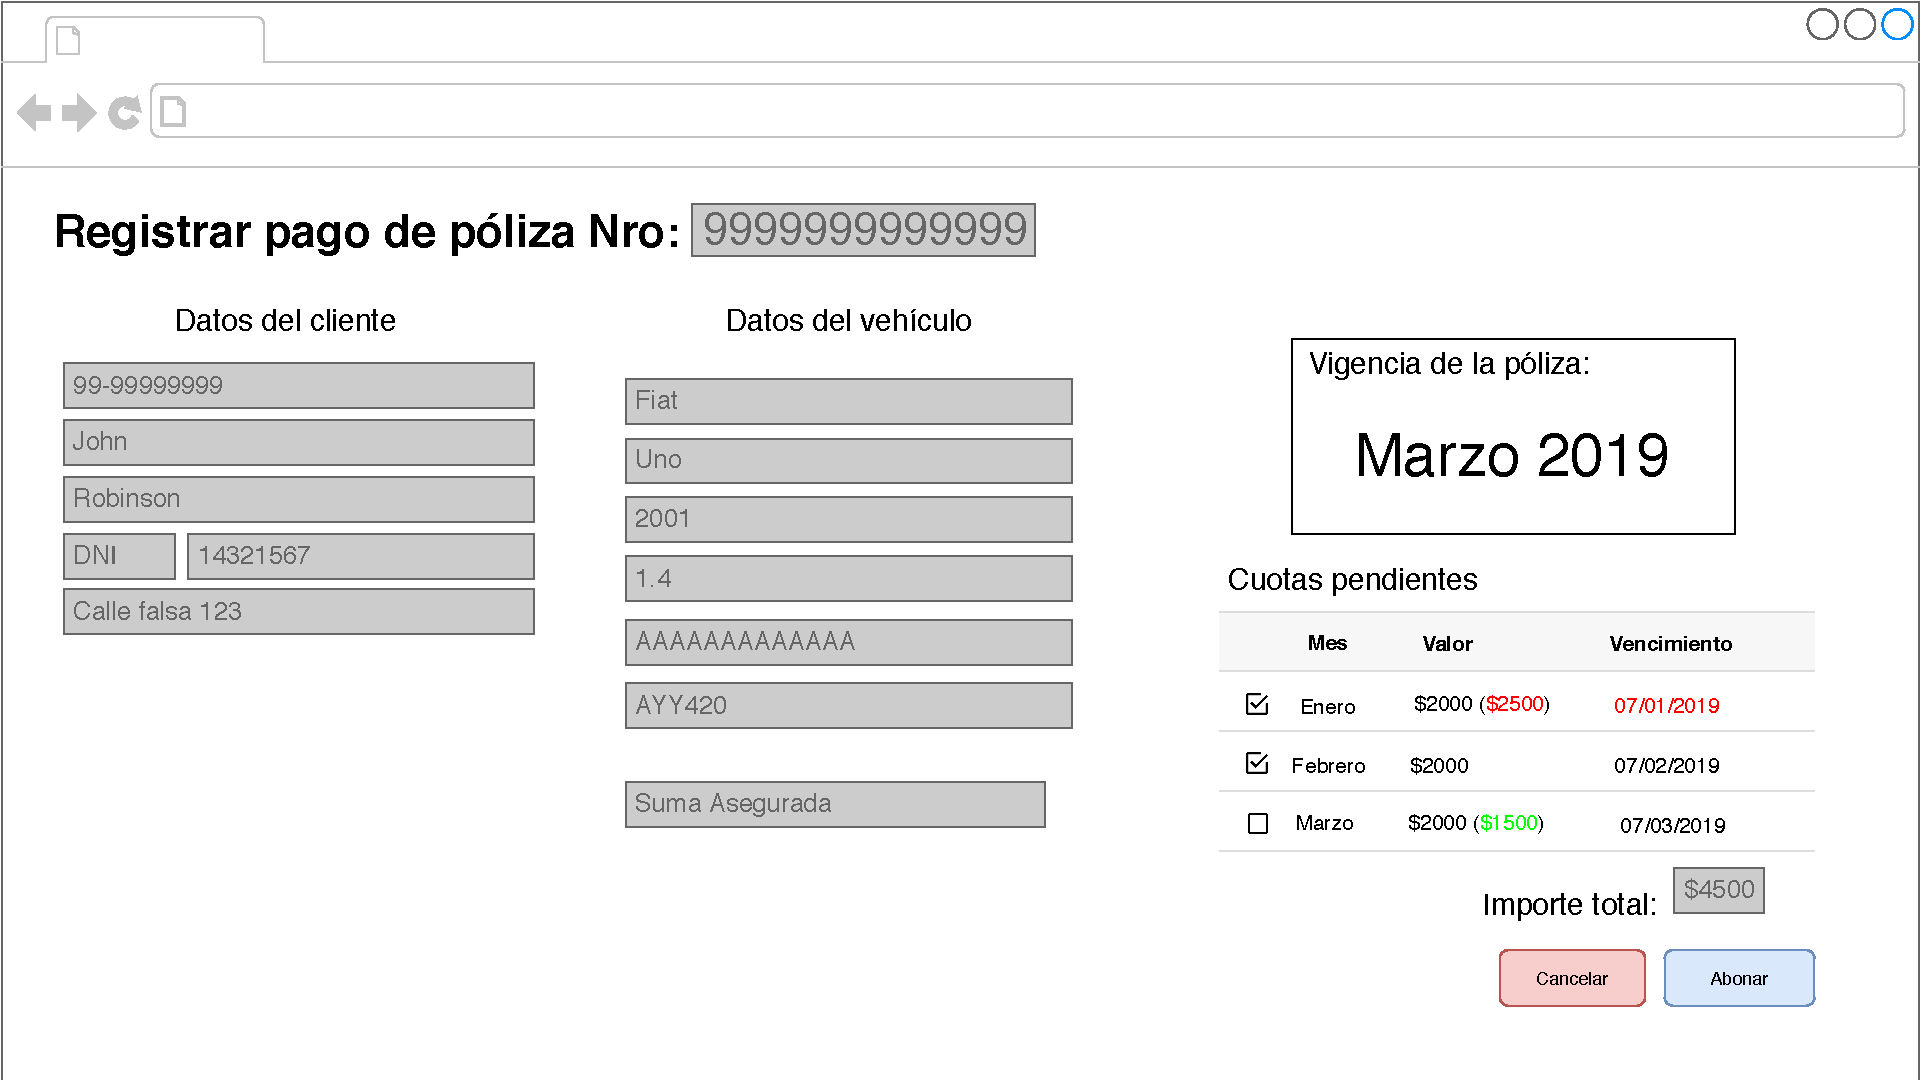
\includegraphics[width=\textwidth]{CU12/CU-121.pdf}
\caption{Caso de uso 12 (flujo principal)}
\end{figure}
\vfill

\vfill
\begin{figure}[h!]
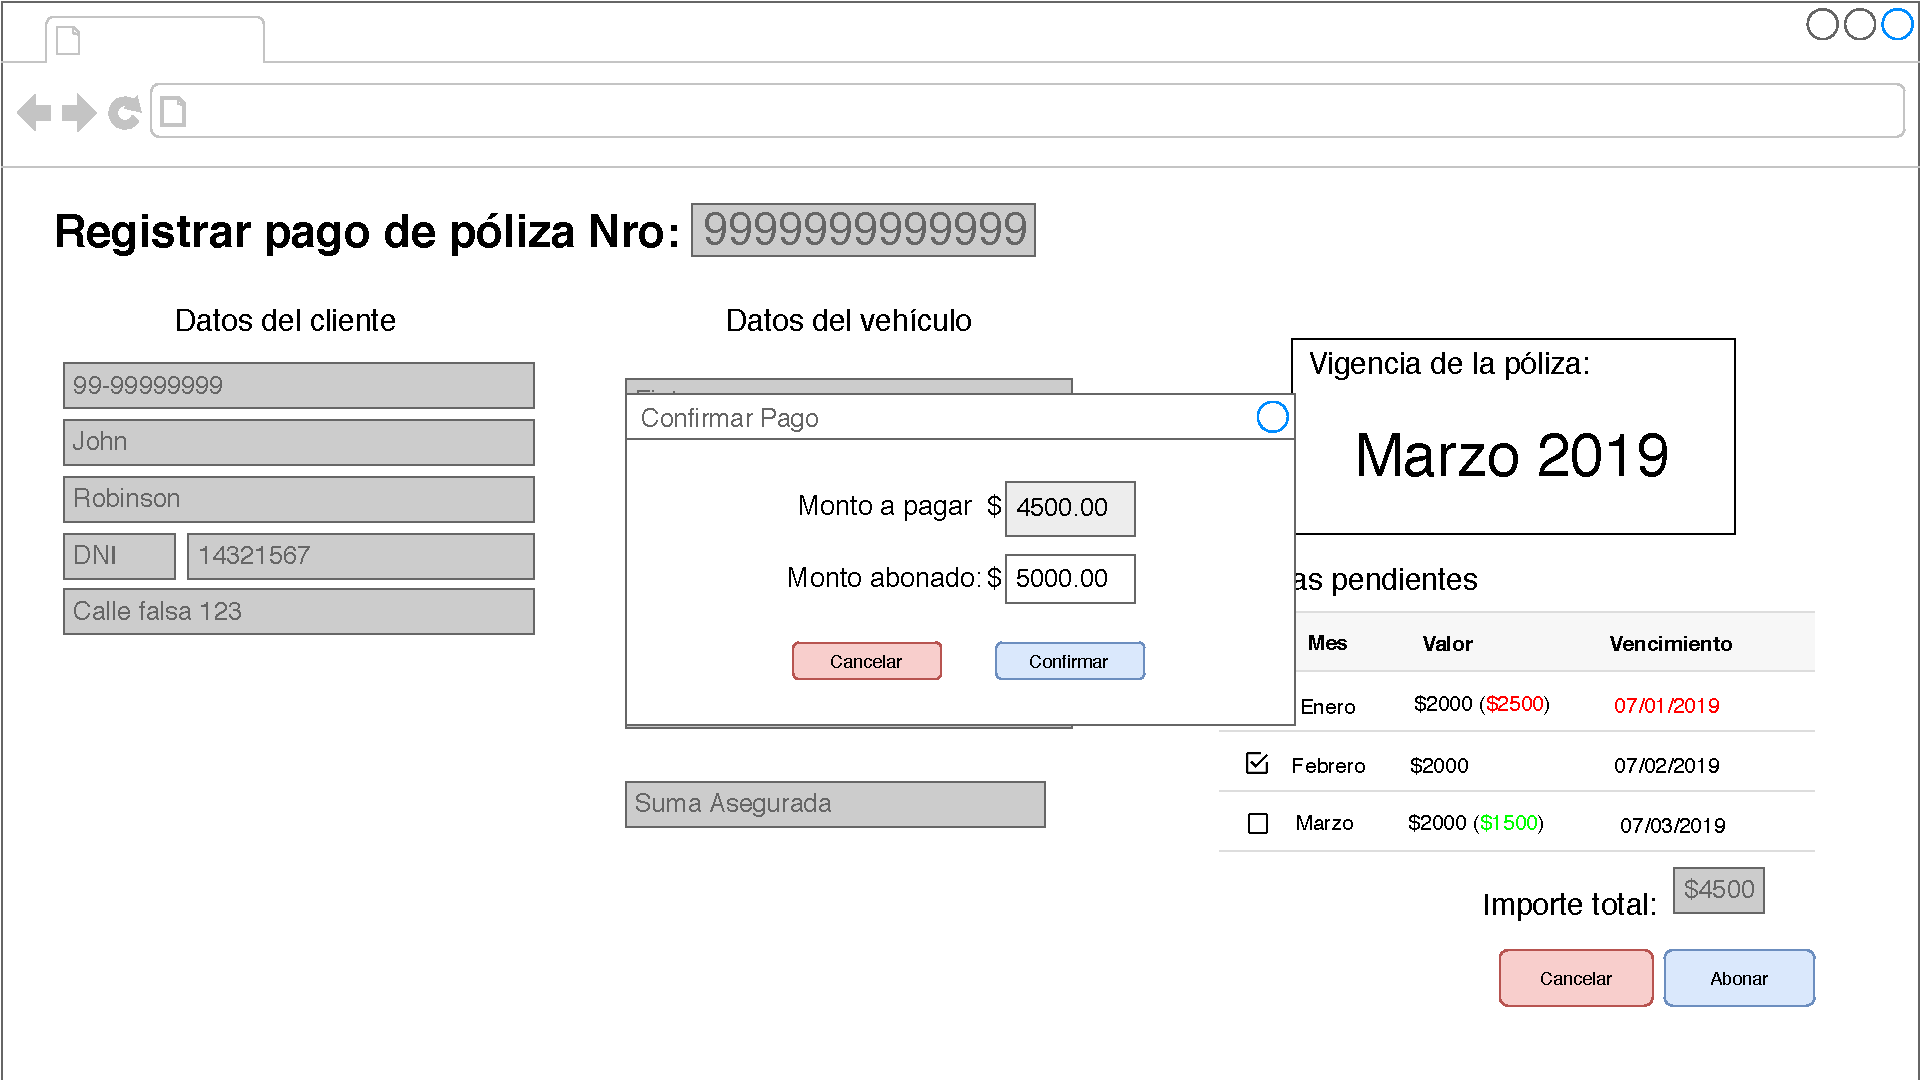
\includegraphics[width=\textwidth]{CU12/CU-122.pdf}
\caption{Caso de uso 12 (flujo principal)}
\end{figure}
\vfill

\vfill
\begin{figure}[h!]
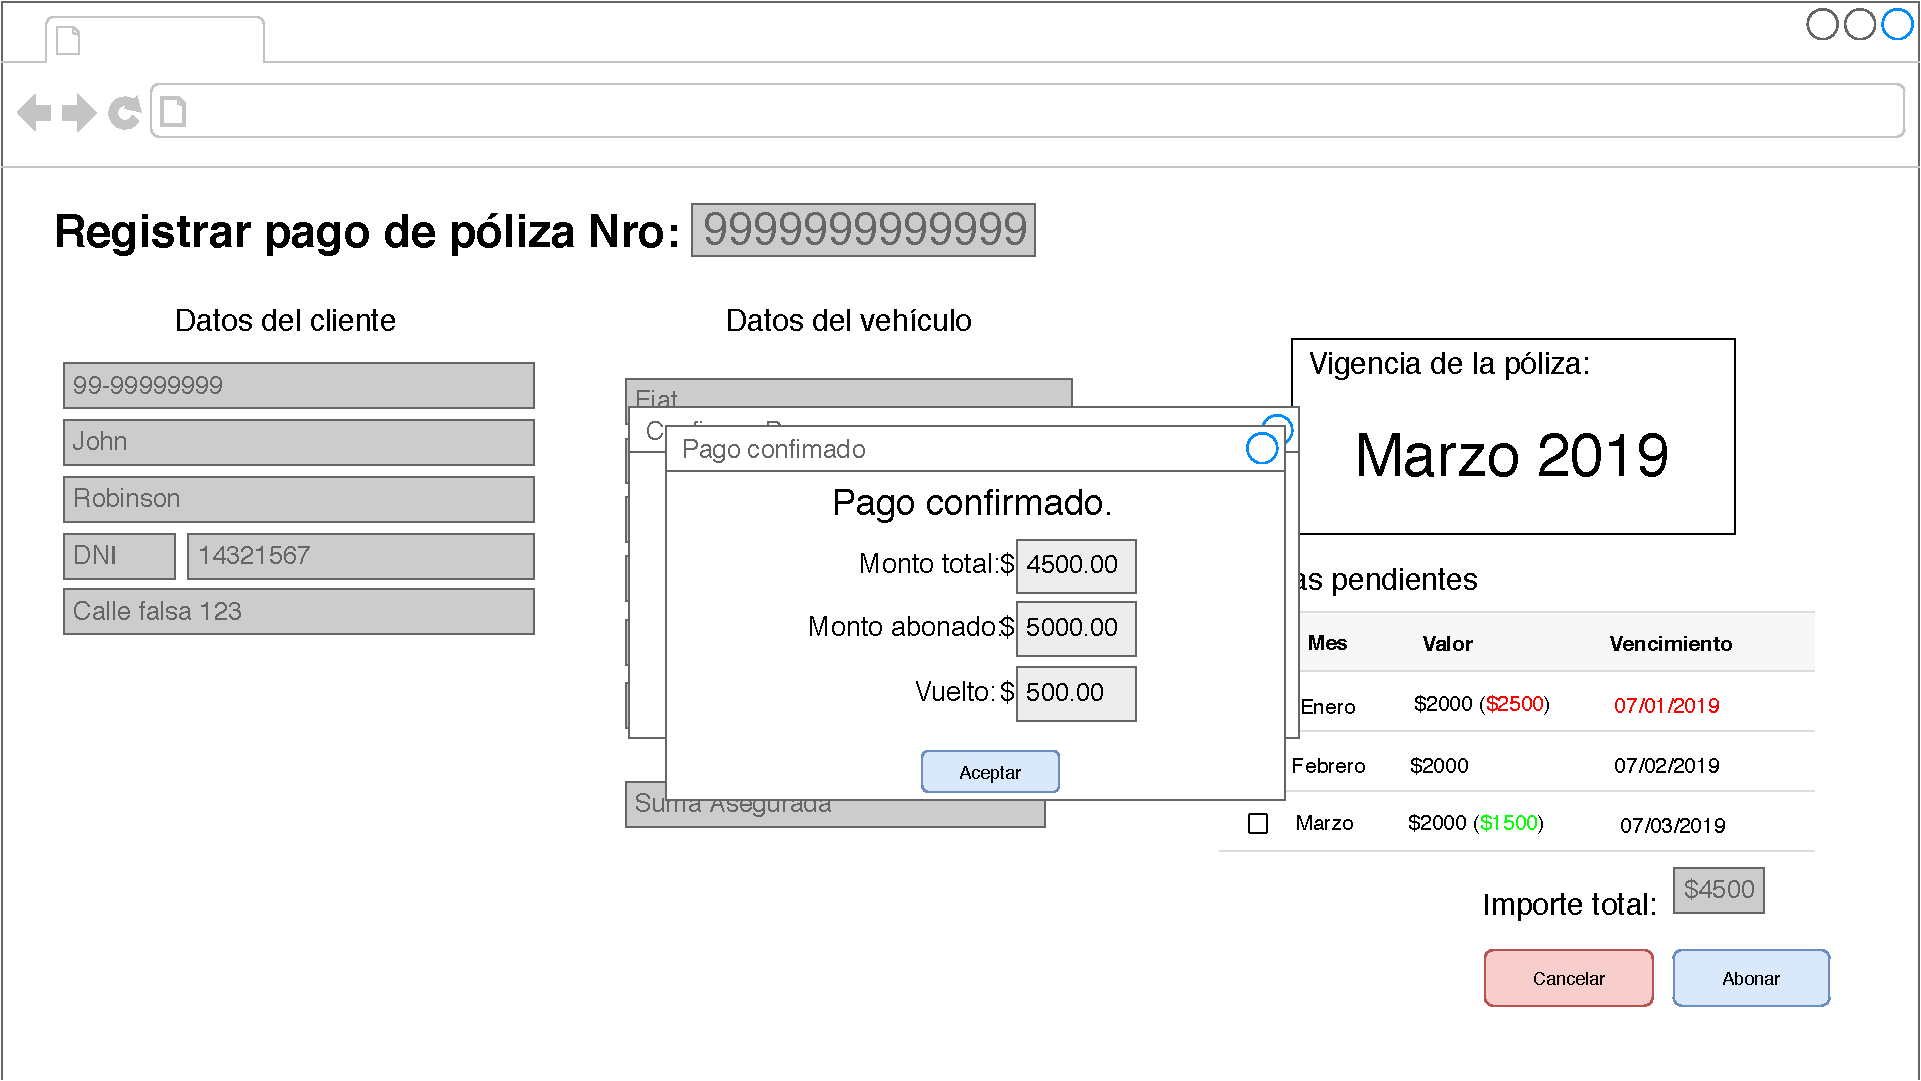
\includegraphics[width=\textwidth]{CU12/CU-123.pdf}
\caption{Caso de uso 12 (flujo principal)}
\end{figure}
\vfill

\vfill
\begin{figure}[h!]
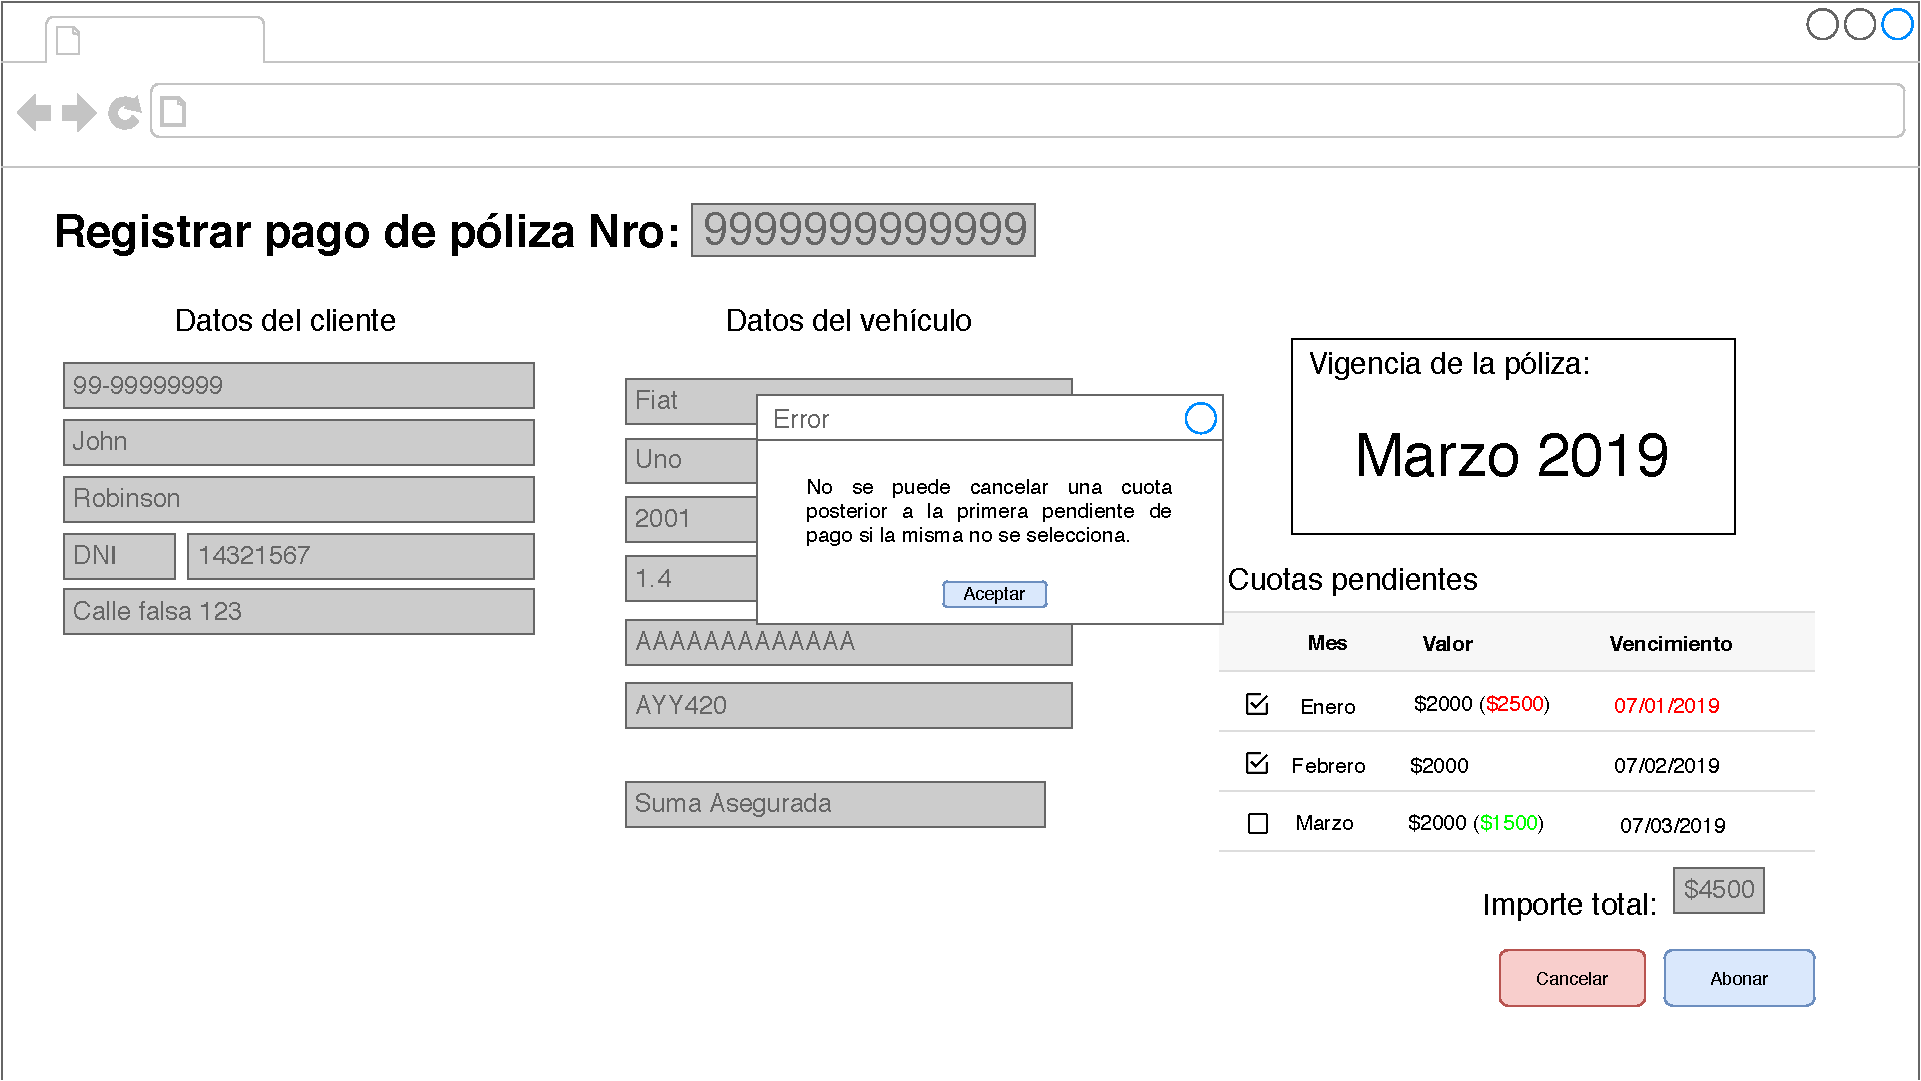
\includegraphics[width=\textwidth]{CU12/CU-124.pdf}
\caption{Caso de uso 12 (operación no permitida)}
\end{figure}
\vfill

%%%%%%%%%%%%%%%%%%%%%%%
%%%%%%        CASO DE USO 14         %%%%%
%%%%%%%%%%%%%%%%%%%%%%%

\vfill
\begin{figure}[h!]
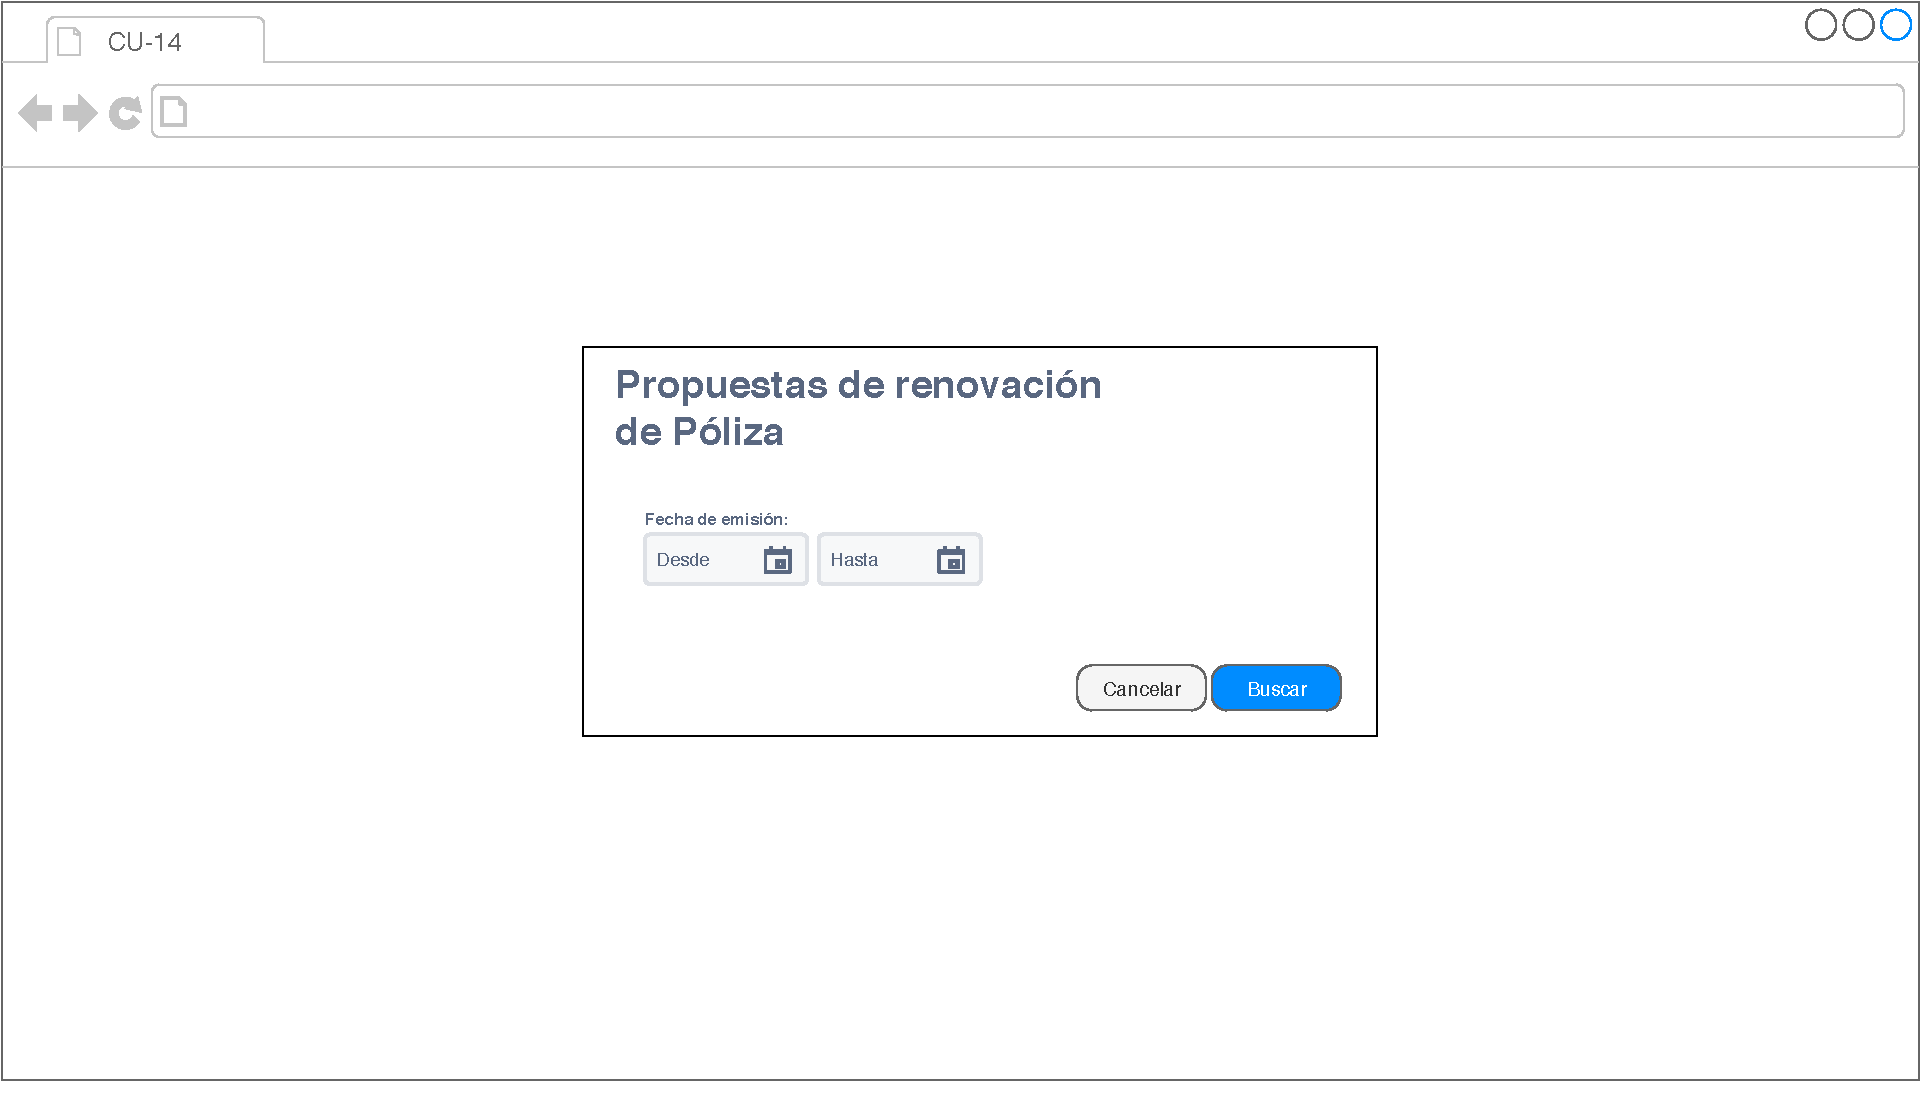
\includegraphics[width=\textwidth]{CU14/CU-141.pdf}
\caption{Caso de uso 14 (flujo principal)}
\end{figure}
\vfill

\vfill
\begin{figure}[h!]
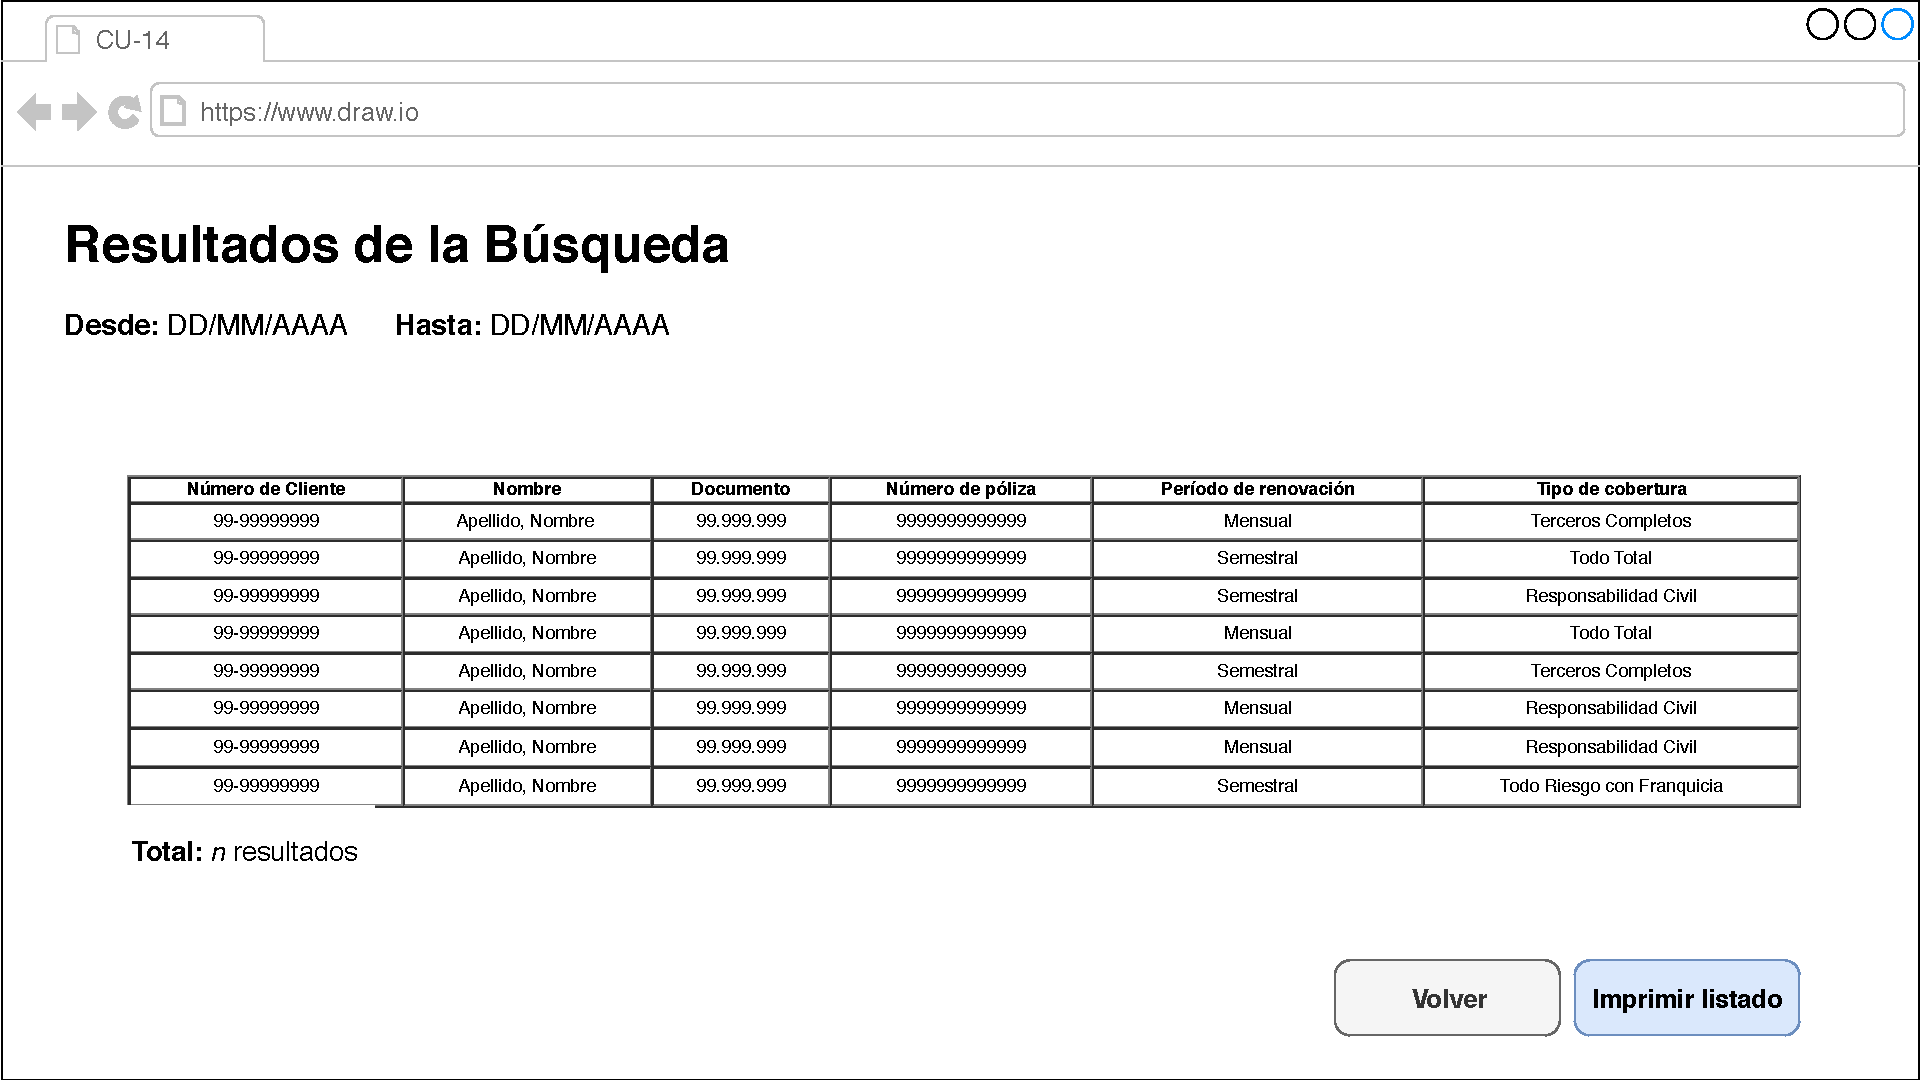
\includegraphics[width=\textwidth]{CU14/CU-142.pdf}
\caption{Caso de uso 14 (flujo principal)}
\end{figure}
\vfill

\vfill
\begin{figure}[h!]
\framebox[\linewidth]{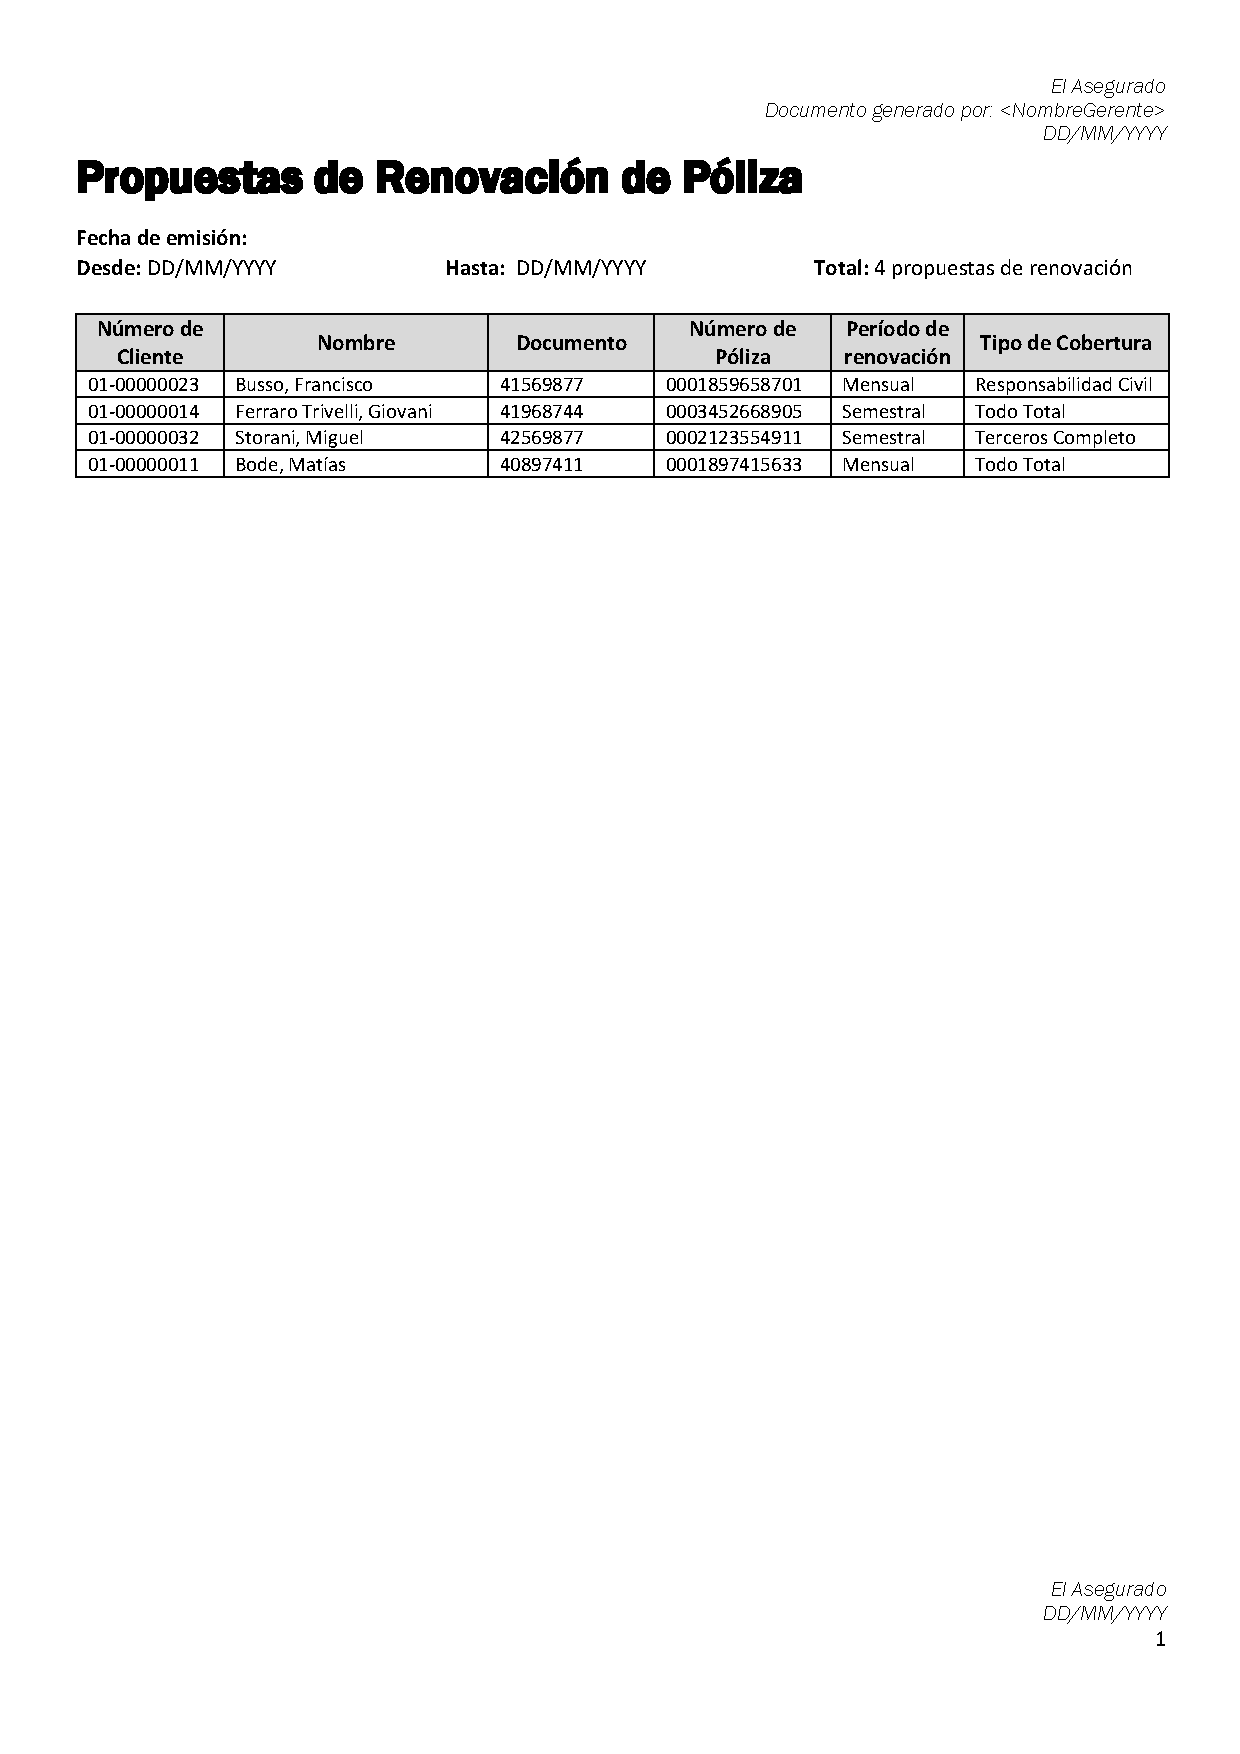
\includegraphics[width=\textwidth]{CU14/CU-14_Listado.pdf}}
\caption{Caso de uso 14 (reporte generado)}
\end{figure}
\vfill



%%%%%%%%%%%%%%%%%%%%%%%
%%%%%%        CASO DE USO 15         %%%%%
%%%%%%%%%%%%%%%%%%%%%%%


\vfill
\begin{figure}[h!]
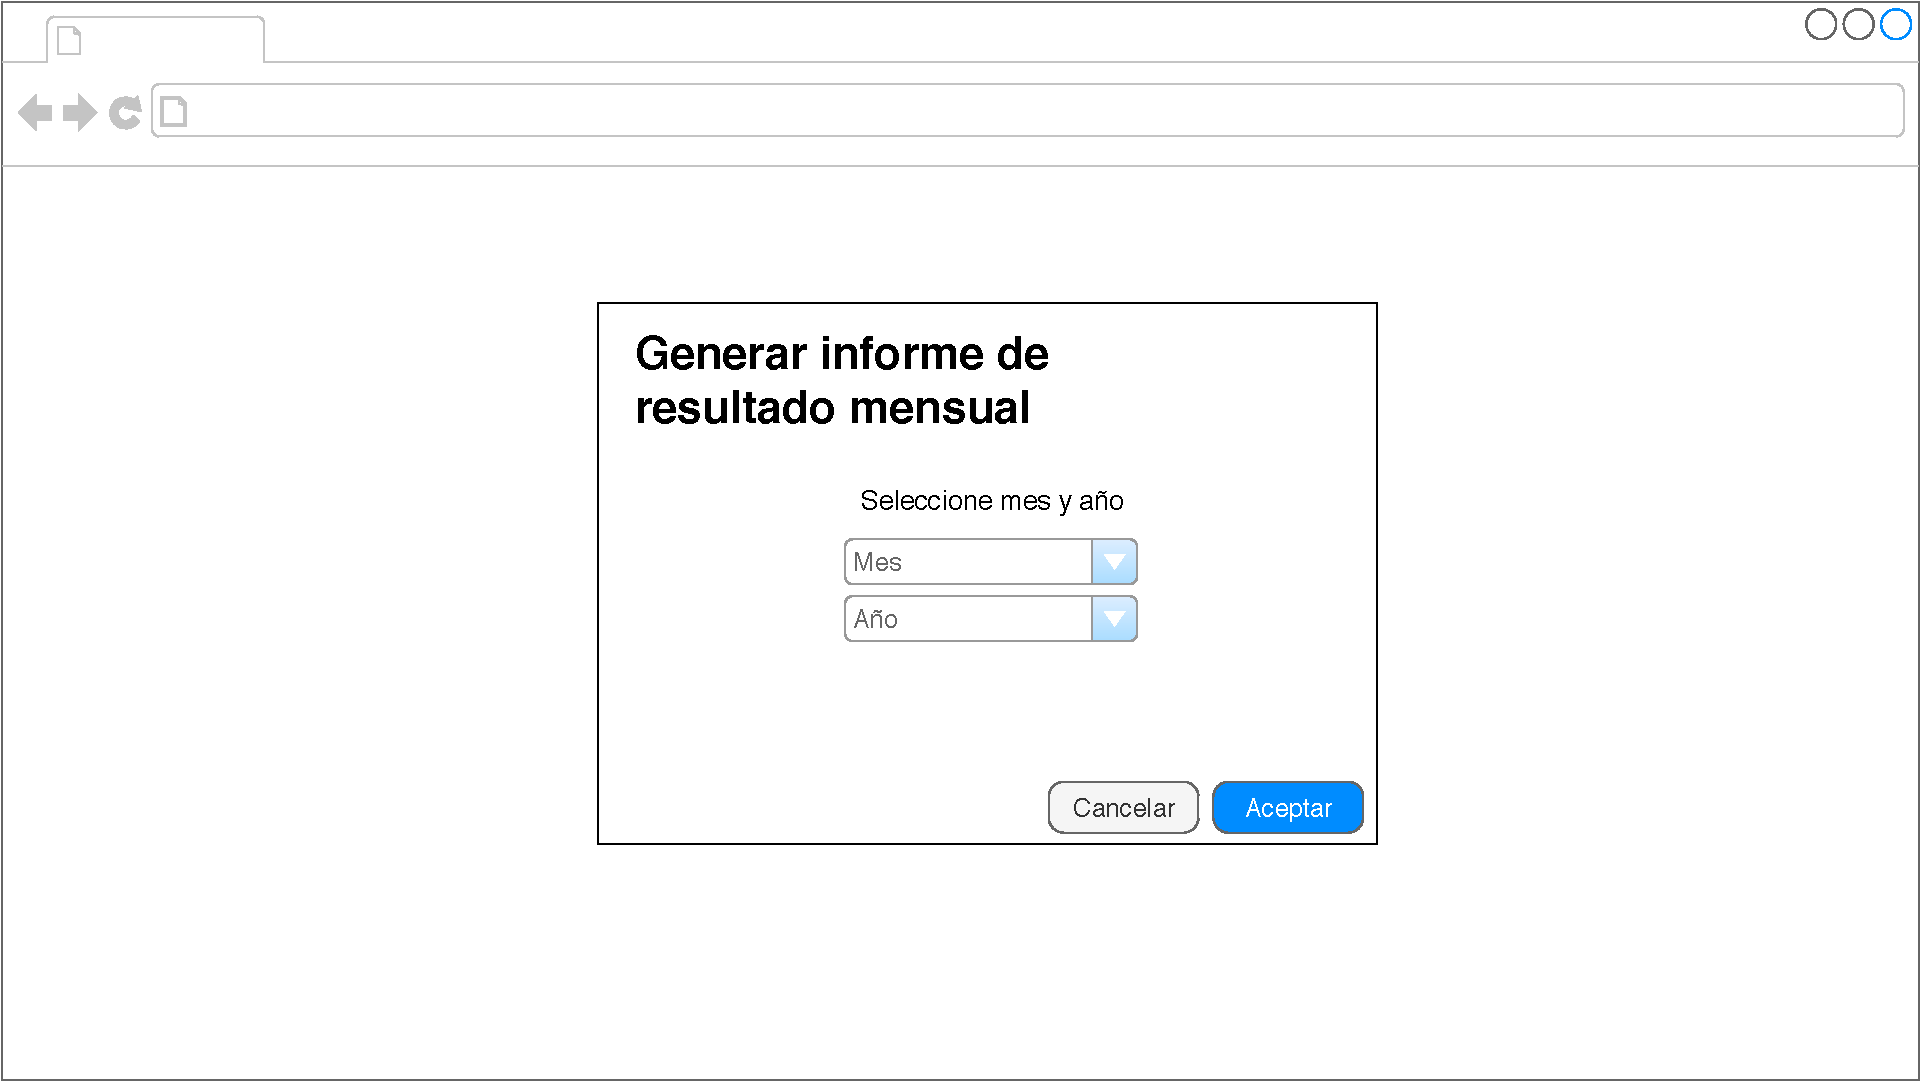
\includegraphics[width=\textwidth]{CU15/CU-151.pdf}
\caption{Caso de uso 15 (flujo principal)}
\end{figure}
\vfill

\vfill
\begin{figure}[h!]
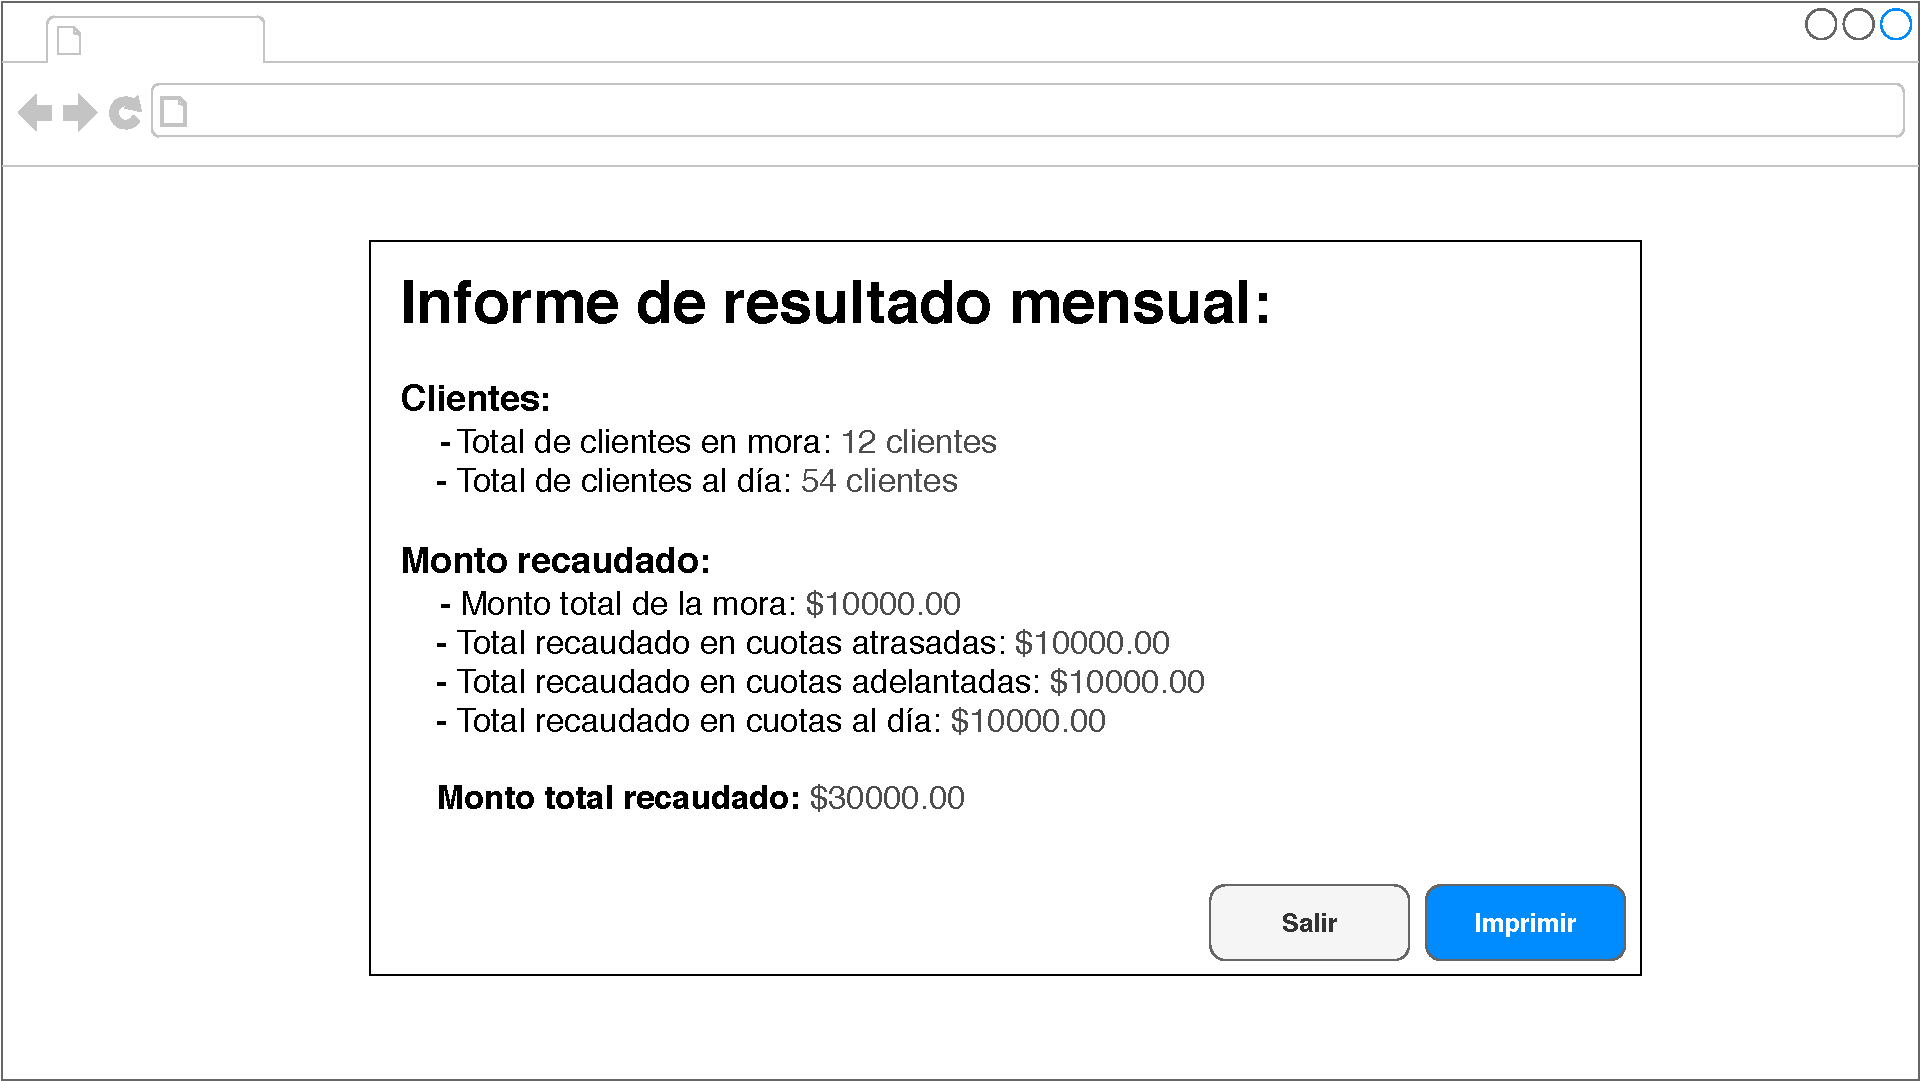
\includegraphics[width=\textwidth]{CU15/CU-152.pdf}
\caption{Caso de uso 15 (flujo principal)}
\end{figure}
\vfill

\vfill
\begin{figure}[h!]
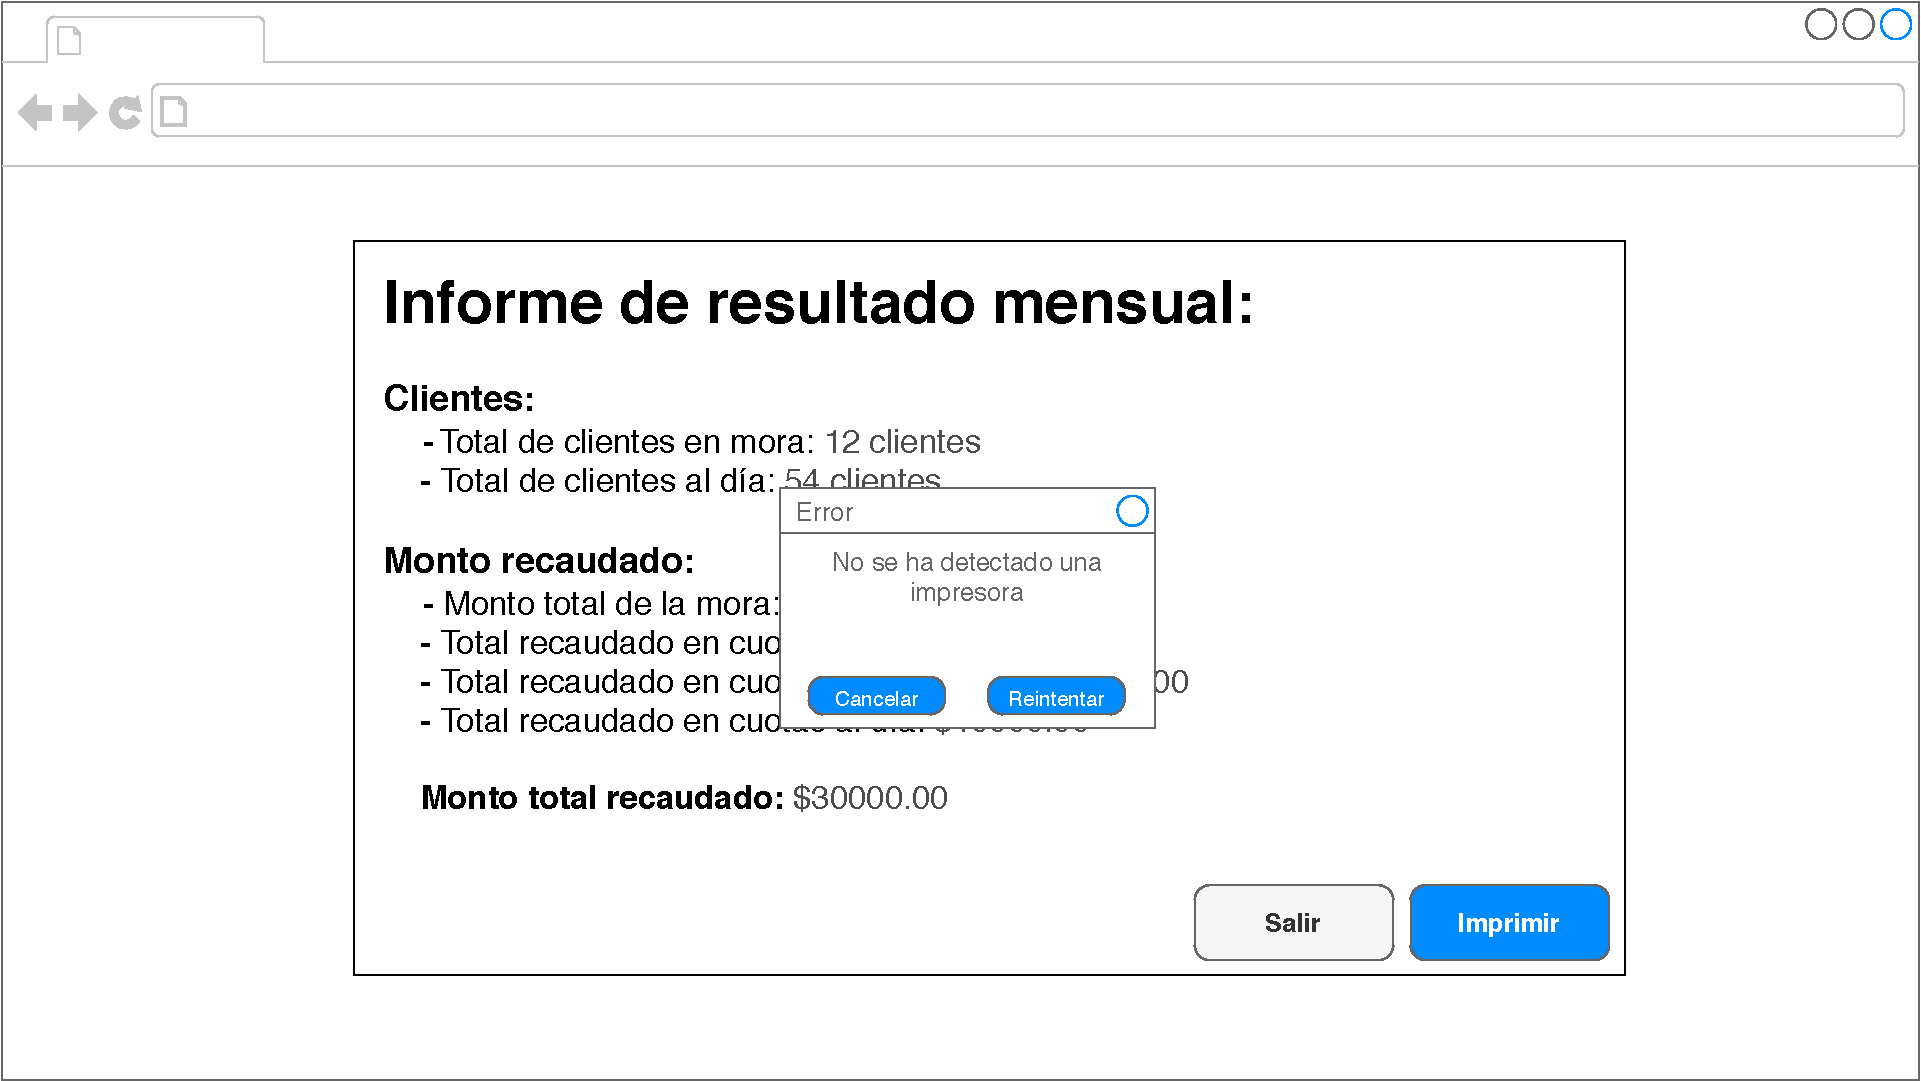
\includegraphics[width=\textwidth]{CU15/CU-153.pdf}
\caption{Caso de uso 15 (no se detecta impresora)}
\end{figure}
\vfill


\begin{figure}[h!]
\framebox[\linewidth]{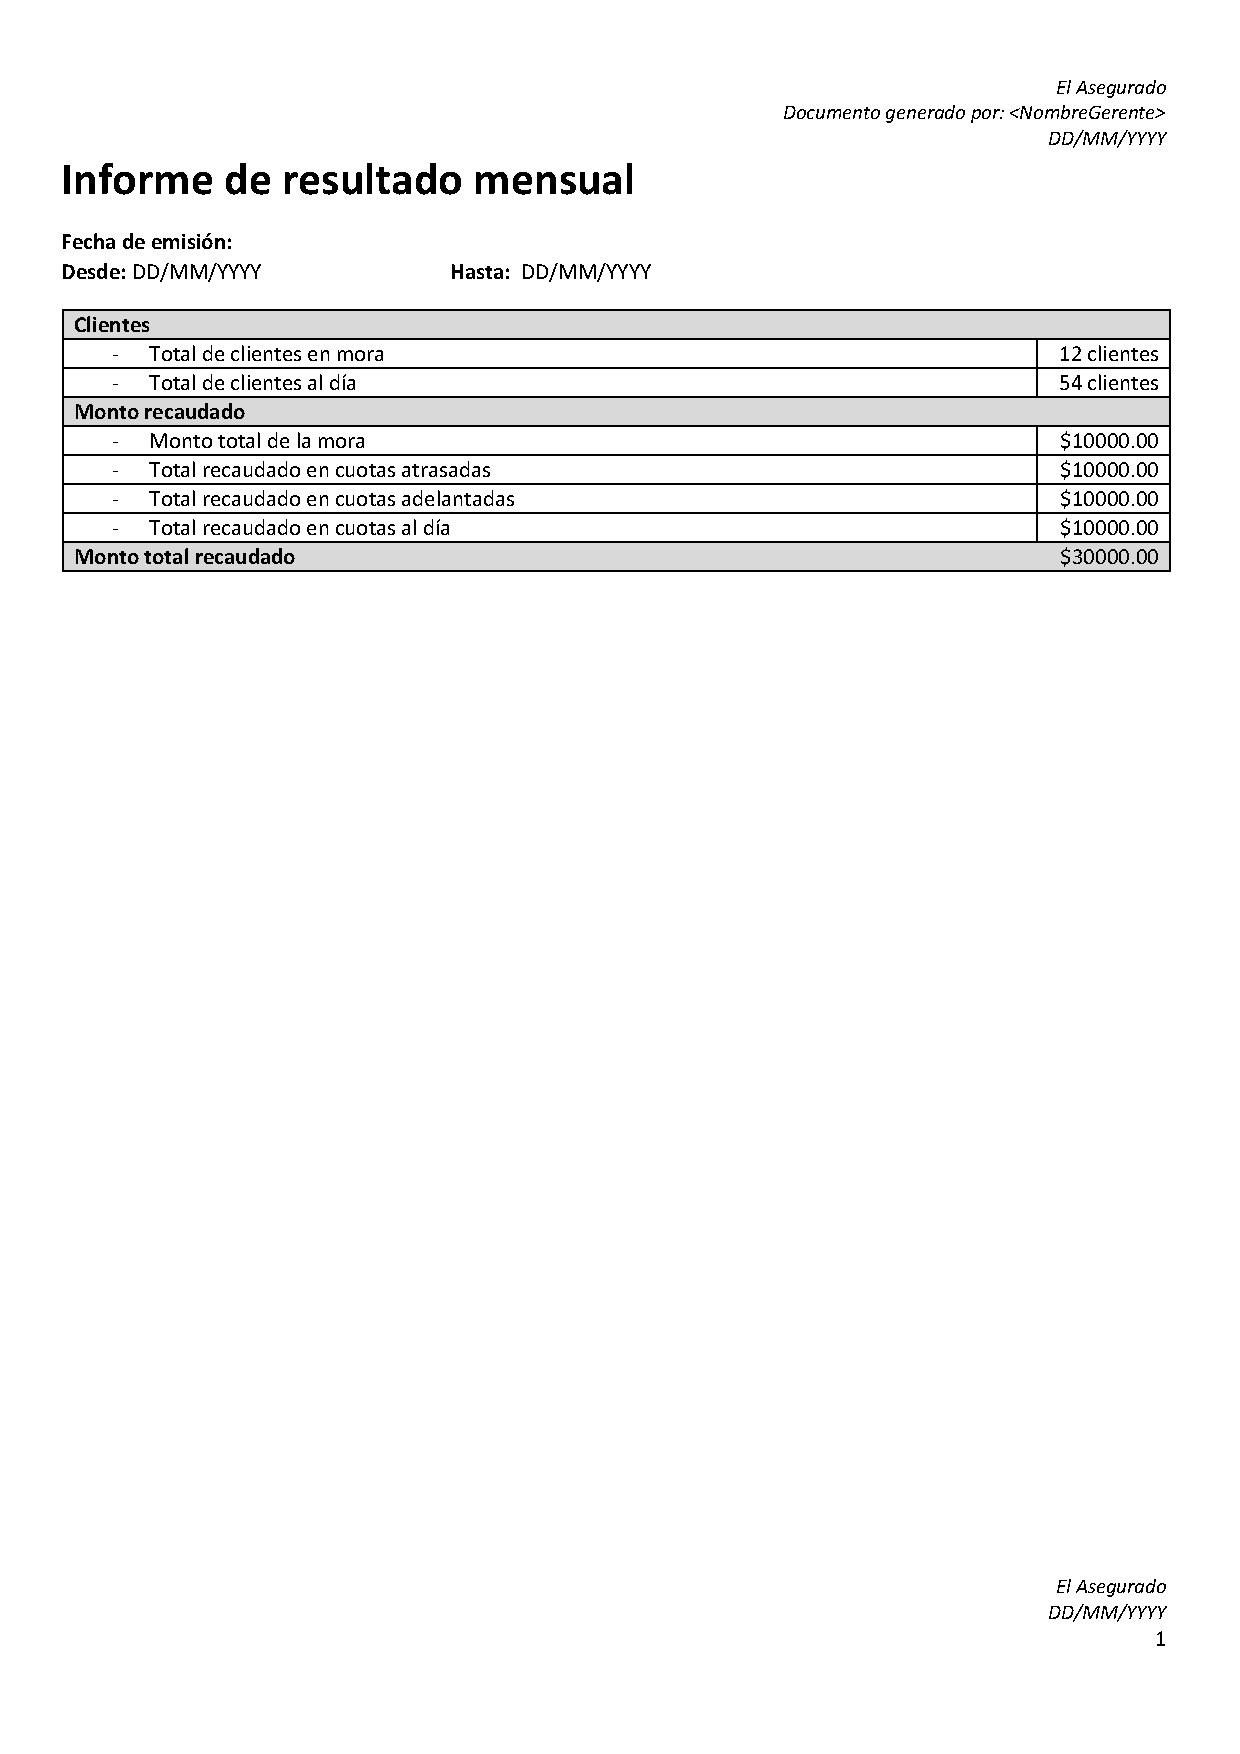
\includegraphics[width=\textwidth]{CU15/CU-15_Listado.pdf}}
\caption{Caso de uso 15 (reporte generado)}
\end{figure}
\vfill

%%%%%%%%%%%%%%%%%%%%%%%
%%%%%%        CASO DE USO 17         %%%%%
%%%%%%%%%%%%%%%%%%%%%%%

\vfill
\begin{figure}[h!]
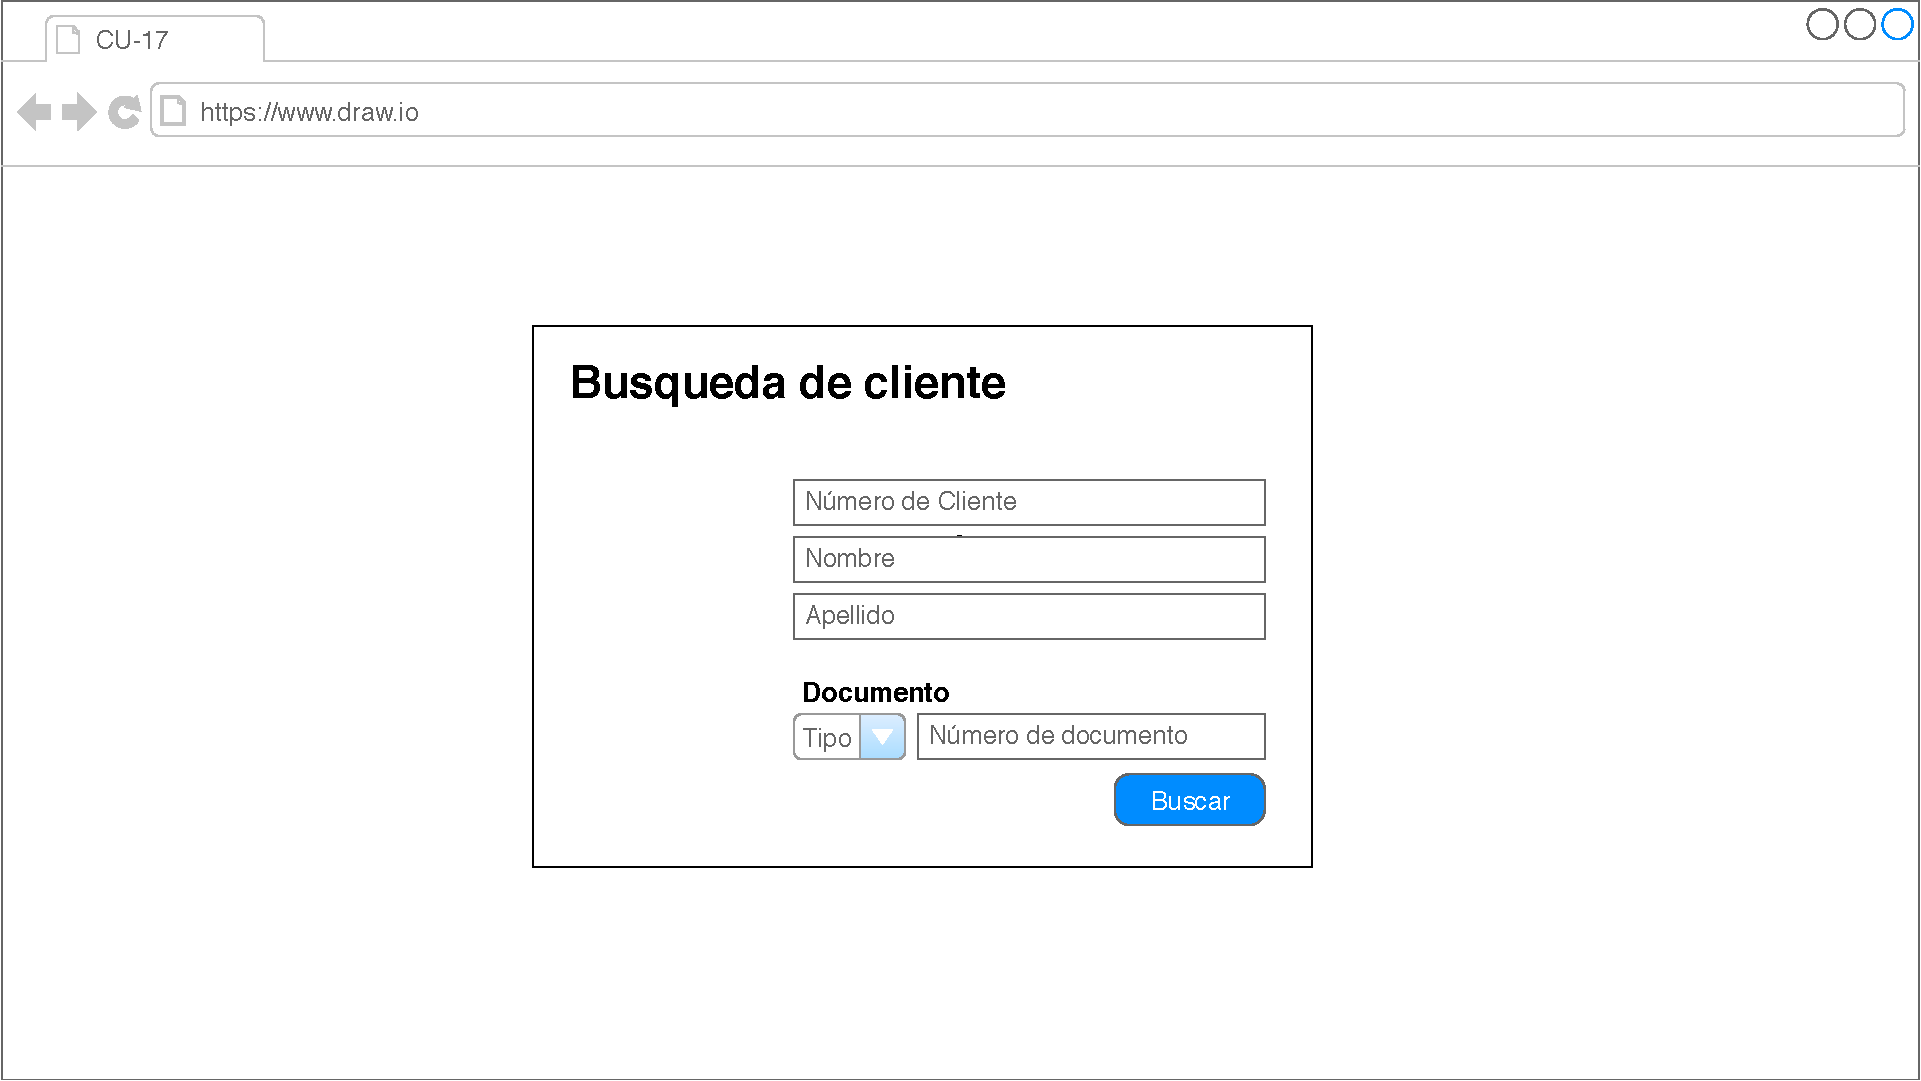
\includegraphics[width=\textwidth]{CU17/CU-171.pdf}
\caption{Caso de uso 17 (flujo principal)}
\end{figure}
\vfill

\vfill
\begin{figure}[h!]
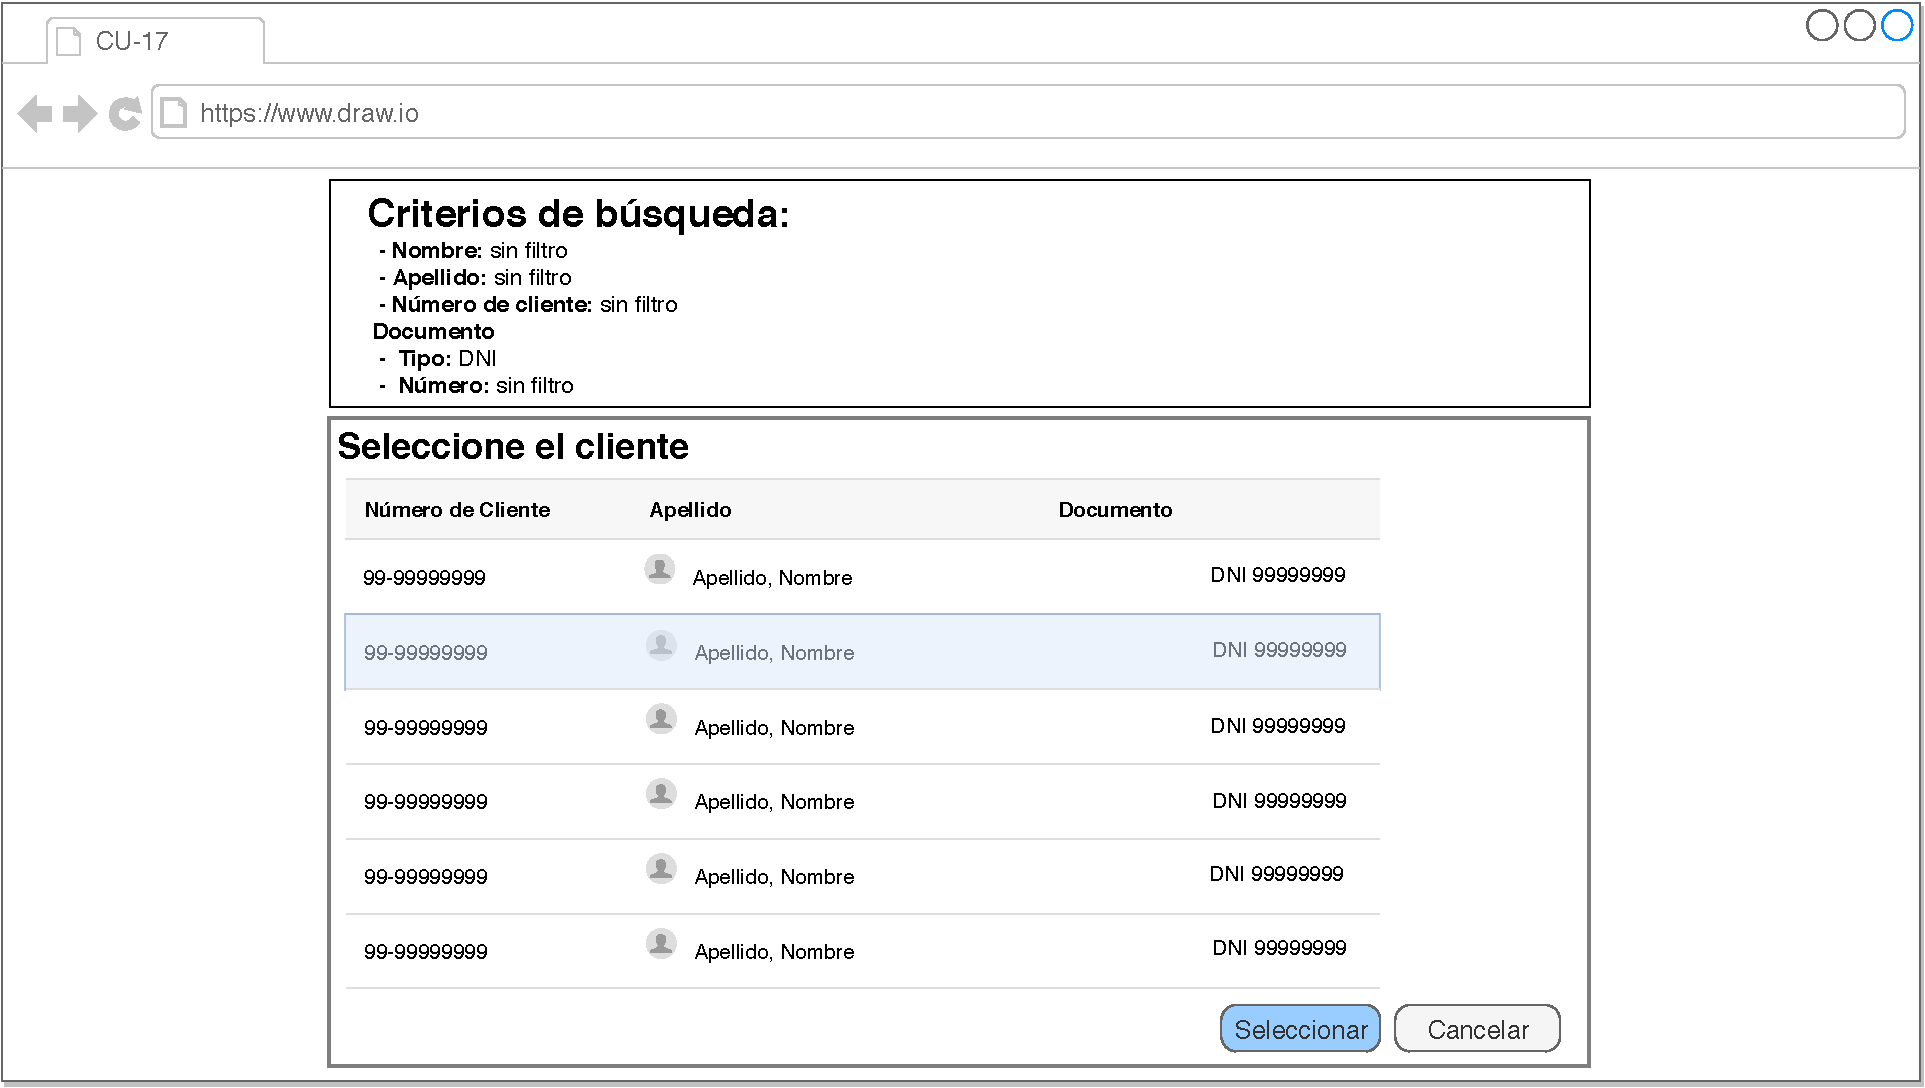
\includegraphics[width=\textwidth]{CU17/CU-172.pdf}
\caption{Caso de uso 17 (flujo principal)}
\end{figure}
\vfill

\vfill
\begin{figure}[h!]
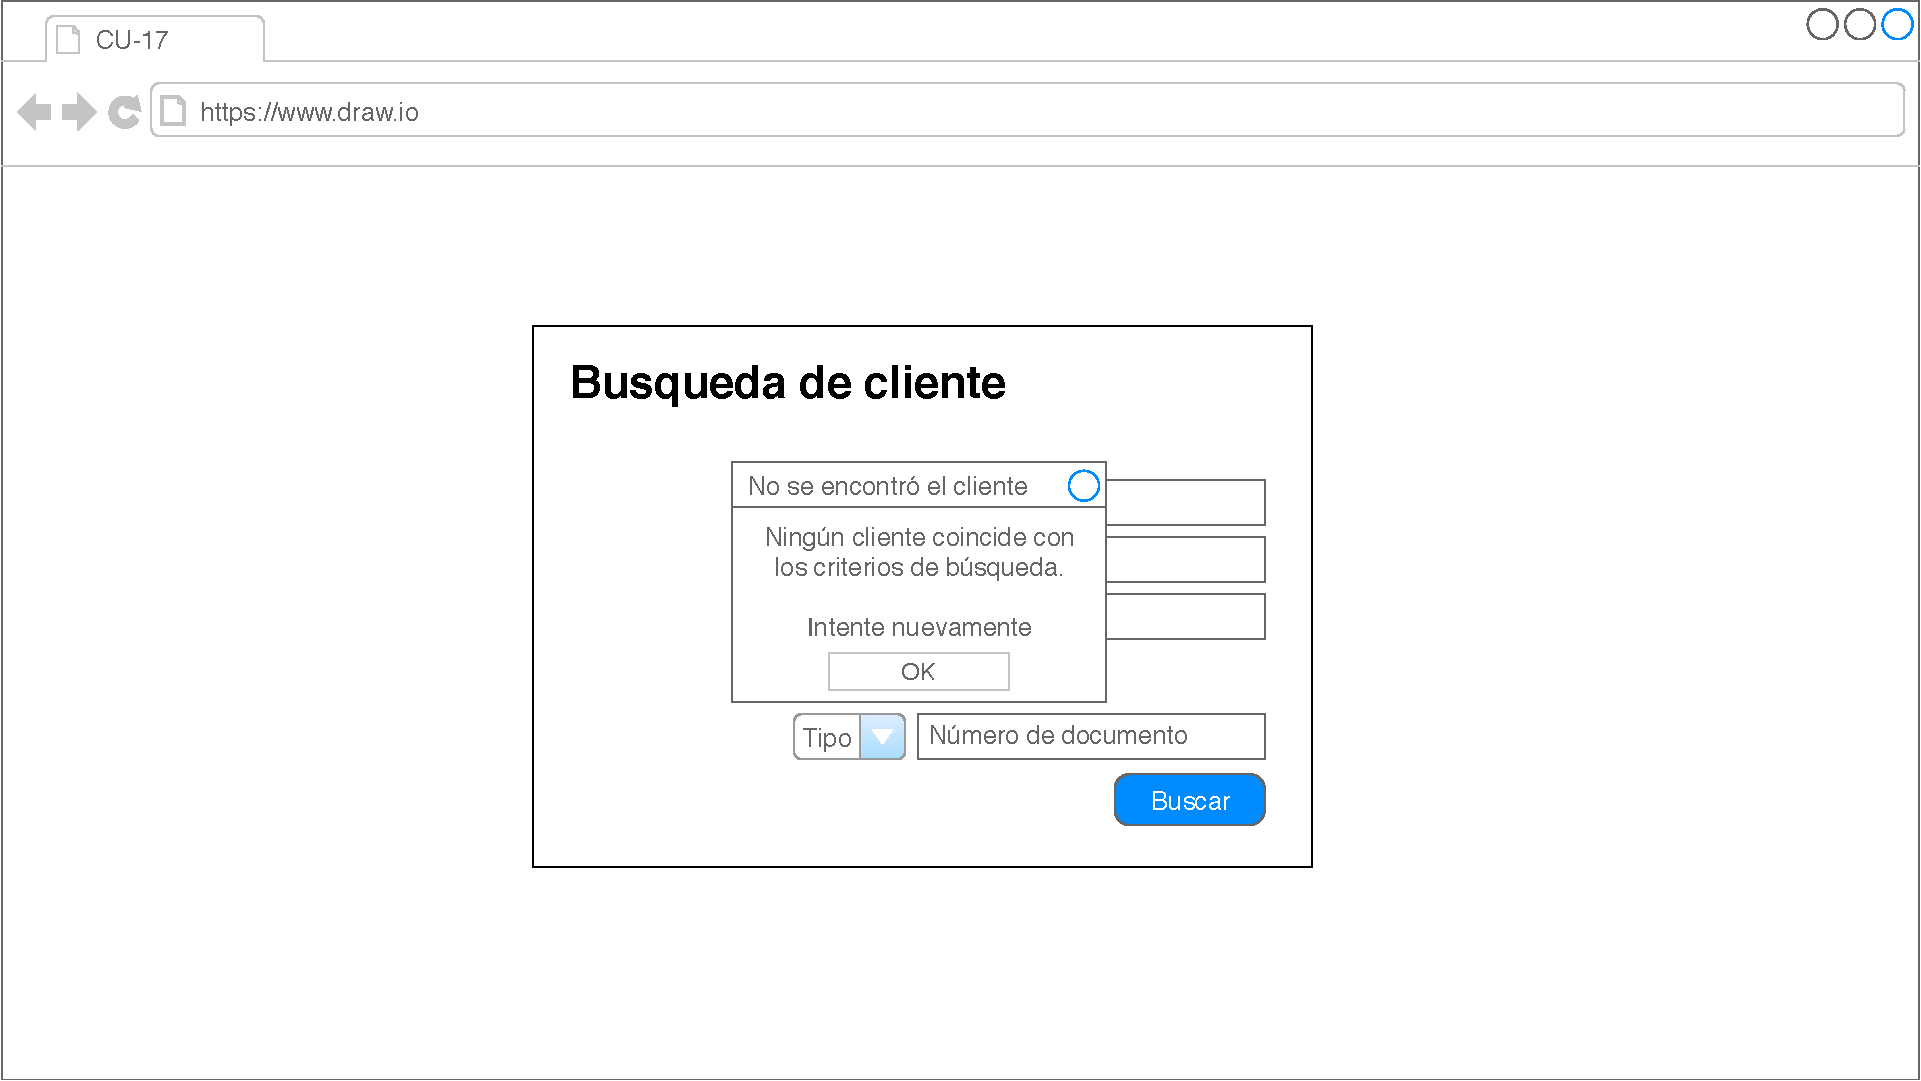
\includegraphics[width=\textwidth]{CU17/CU-173.pdf}
\caption{Caso de uso 17 (no se encuentran clientes)}
\end{figure}
\vfill


%%%%%%%%%%%%%%%%%%%%%%%
%%%%%%        CASO DE USO 18         %%%%%
%%%%%%%%%%%%%%%%%%%%%%%


\vfill
\begin{figure}[h!]
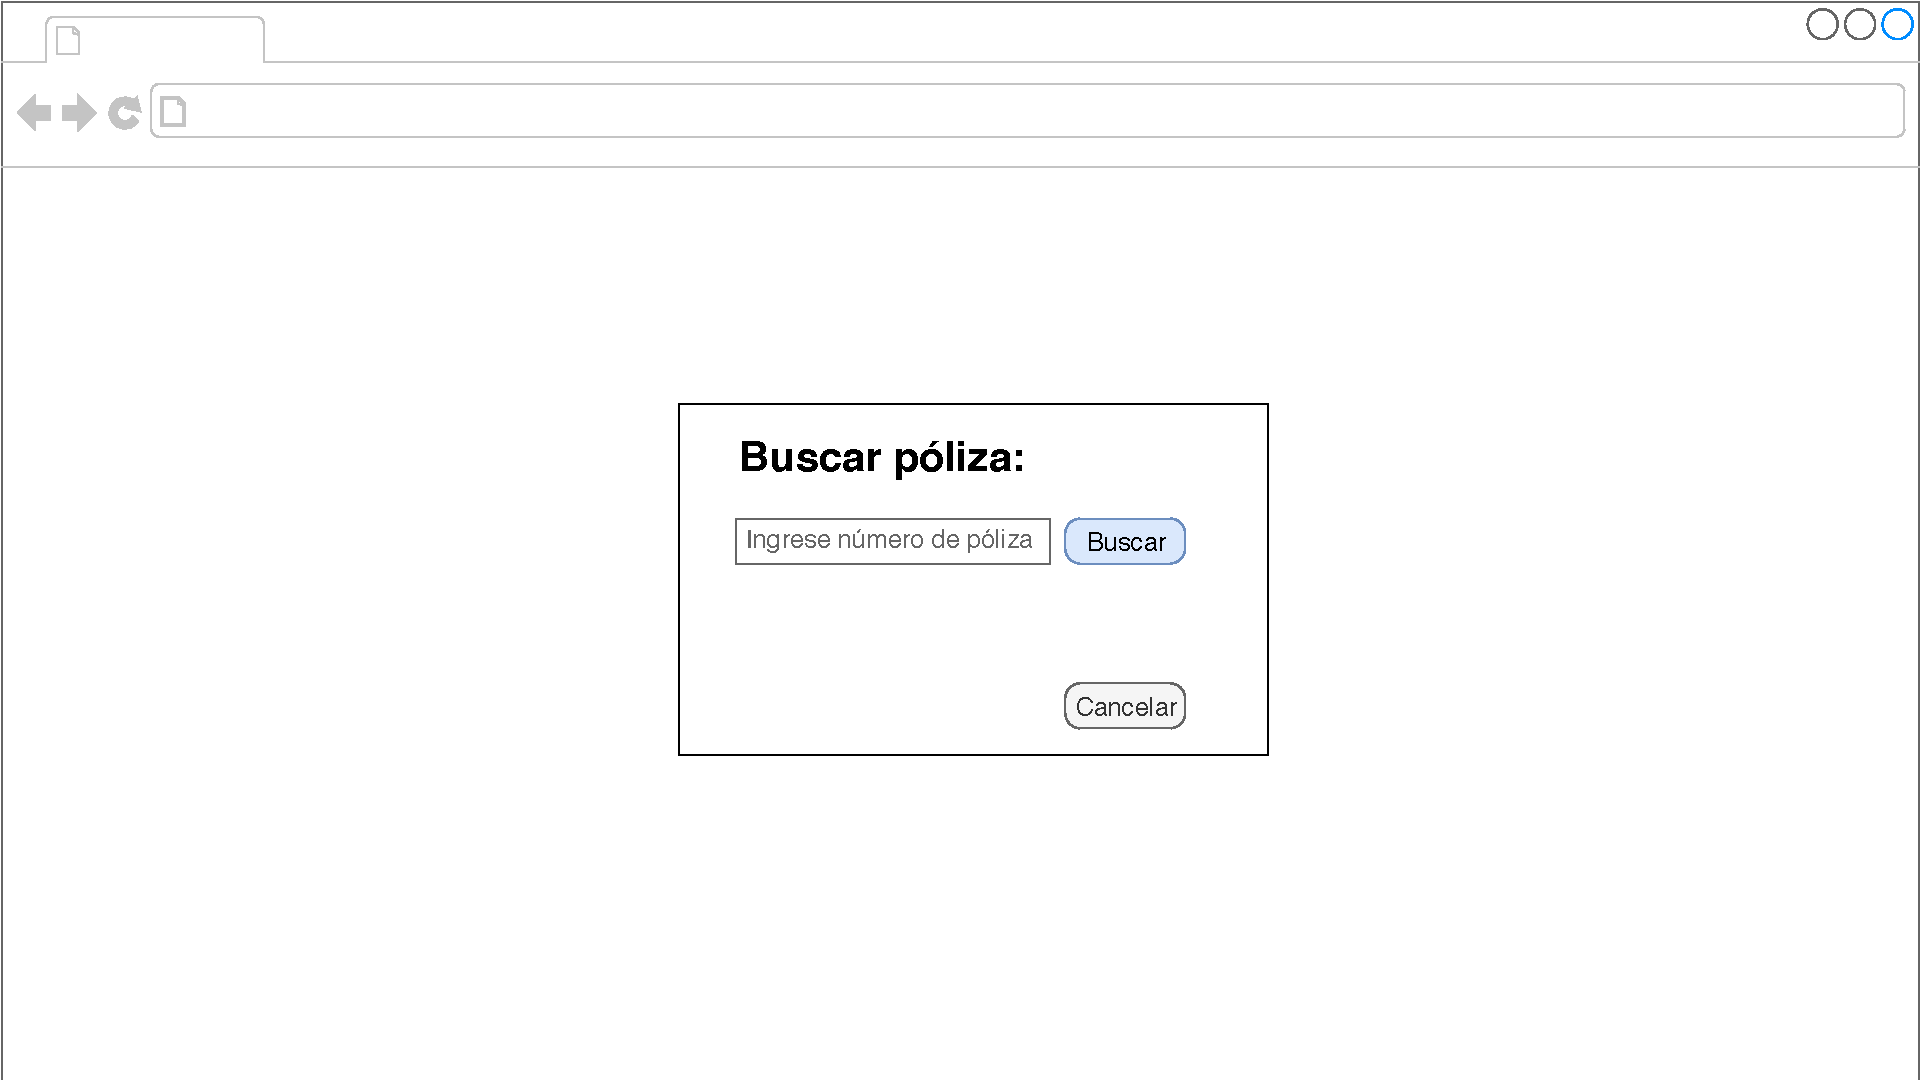
\includegraphics[width=\textwidth]{CU18/CU-181.pdf}
\caption{Caso de uso 18 (flujo principal)}
\end{figure}
\vfill

\vfill
\begin{figure}[h!]
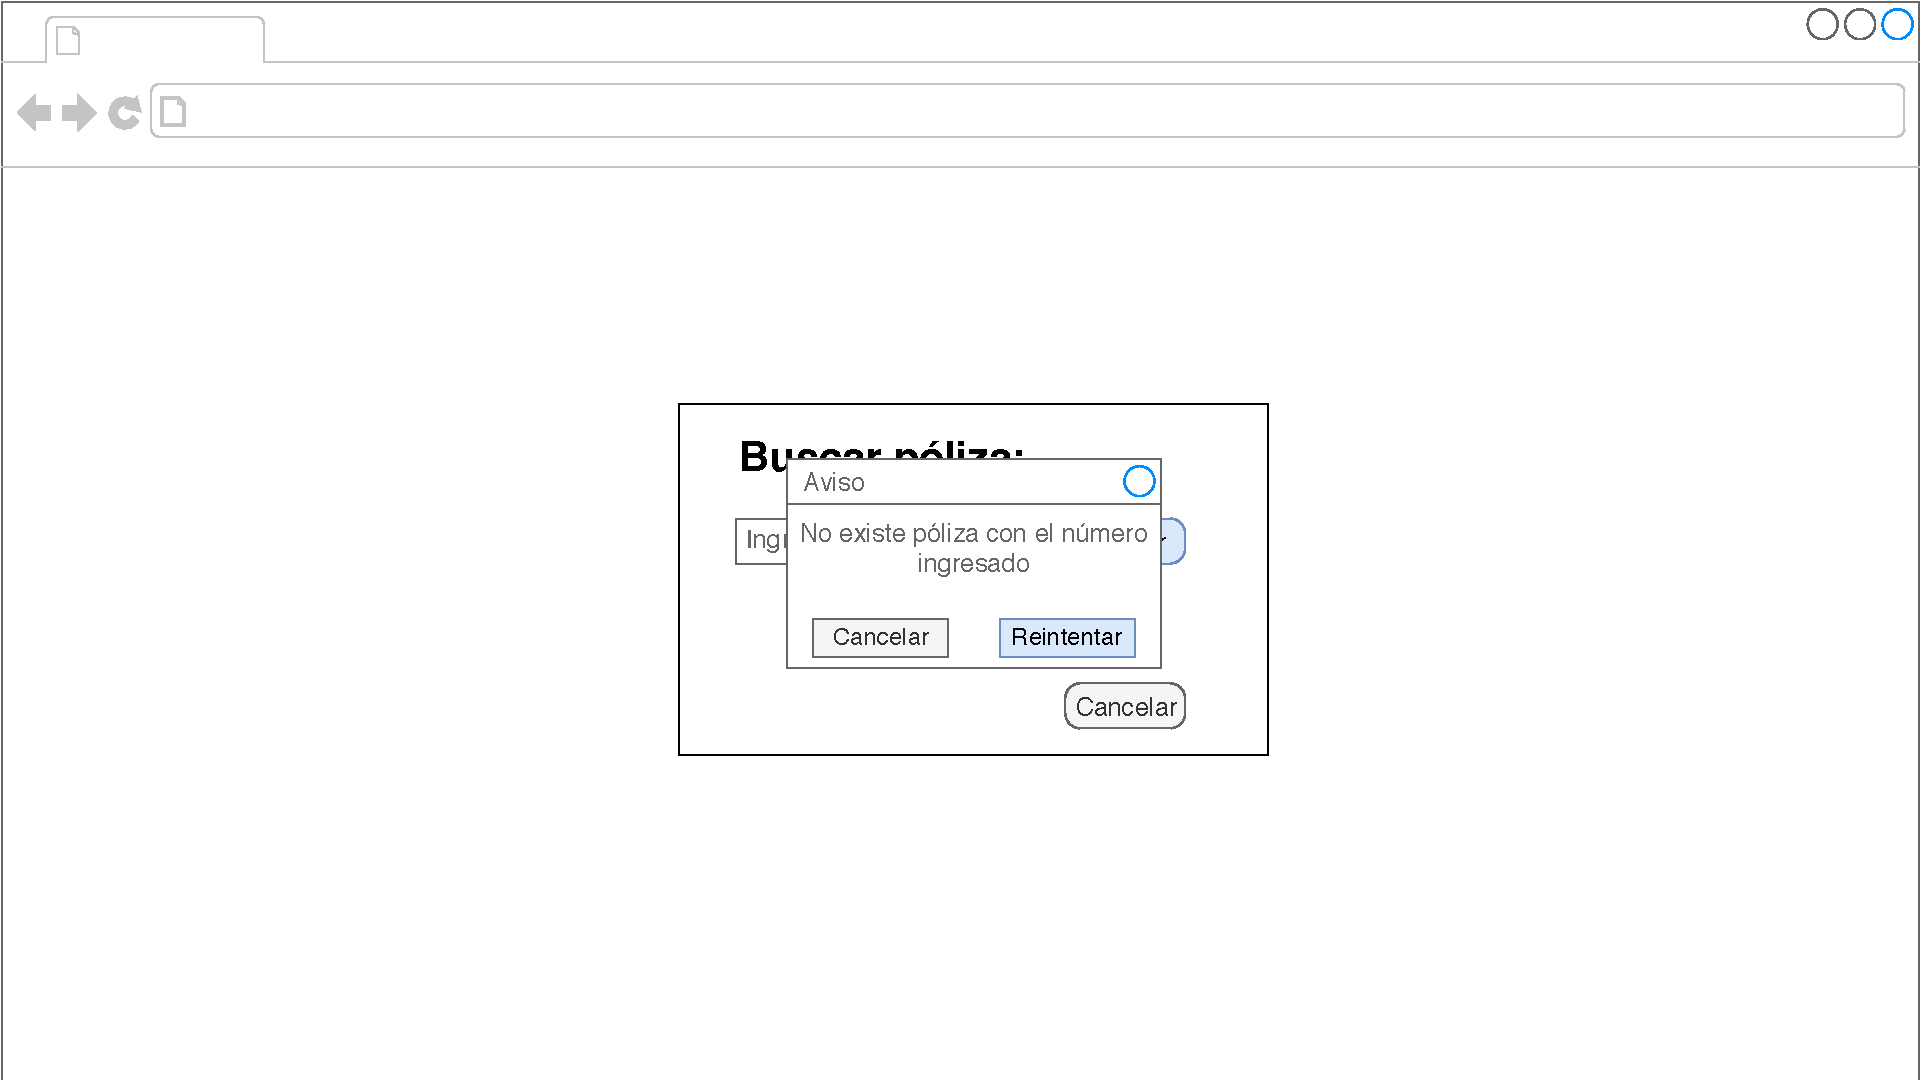
\includegraphics[width=\textwidth]{CU18/CU-182.pdf}
\caption{Caso de uso 18 (no se encuentran pólizas)}
\end{figure}
\vfill

\vfill
\begin{figure}[h!]
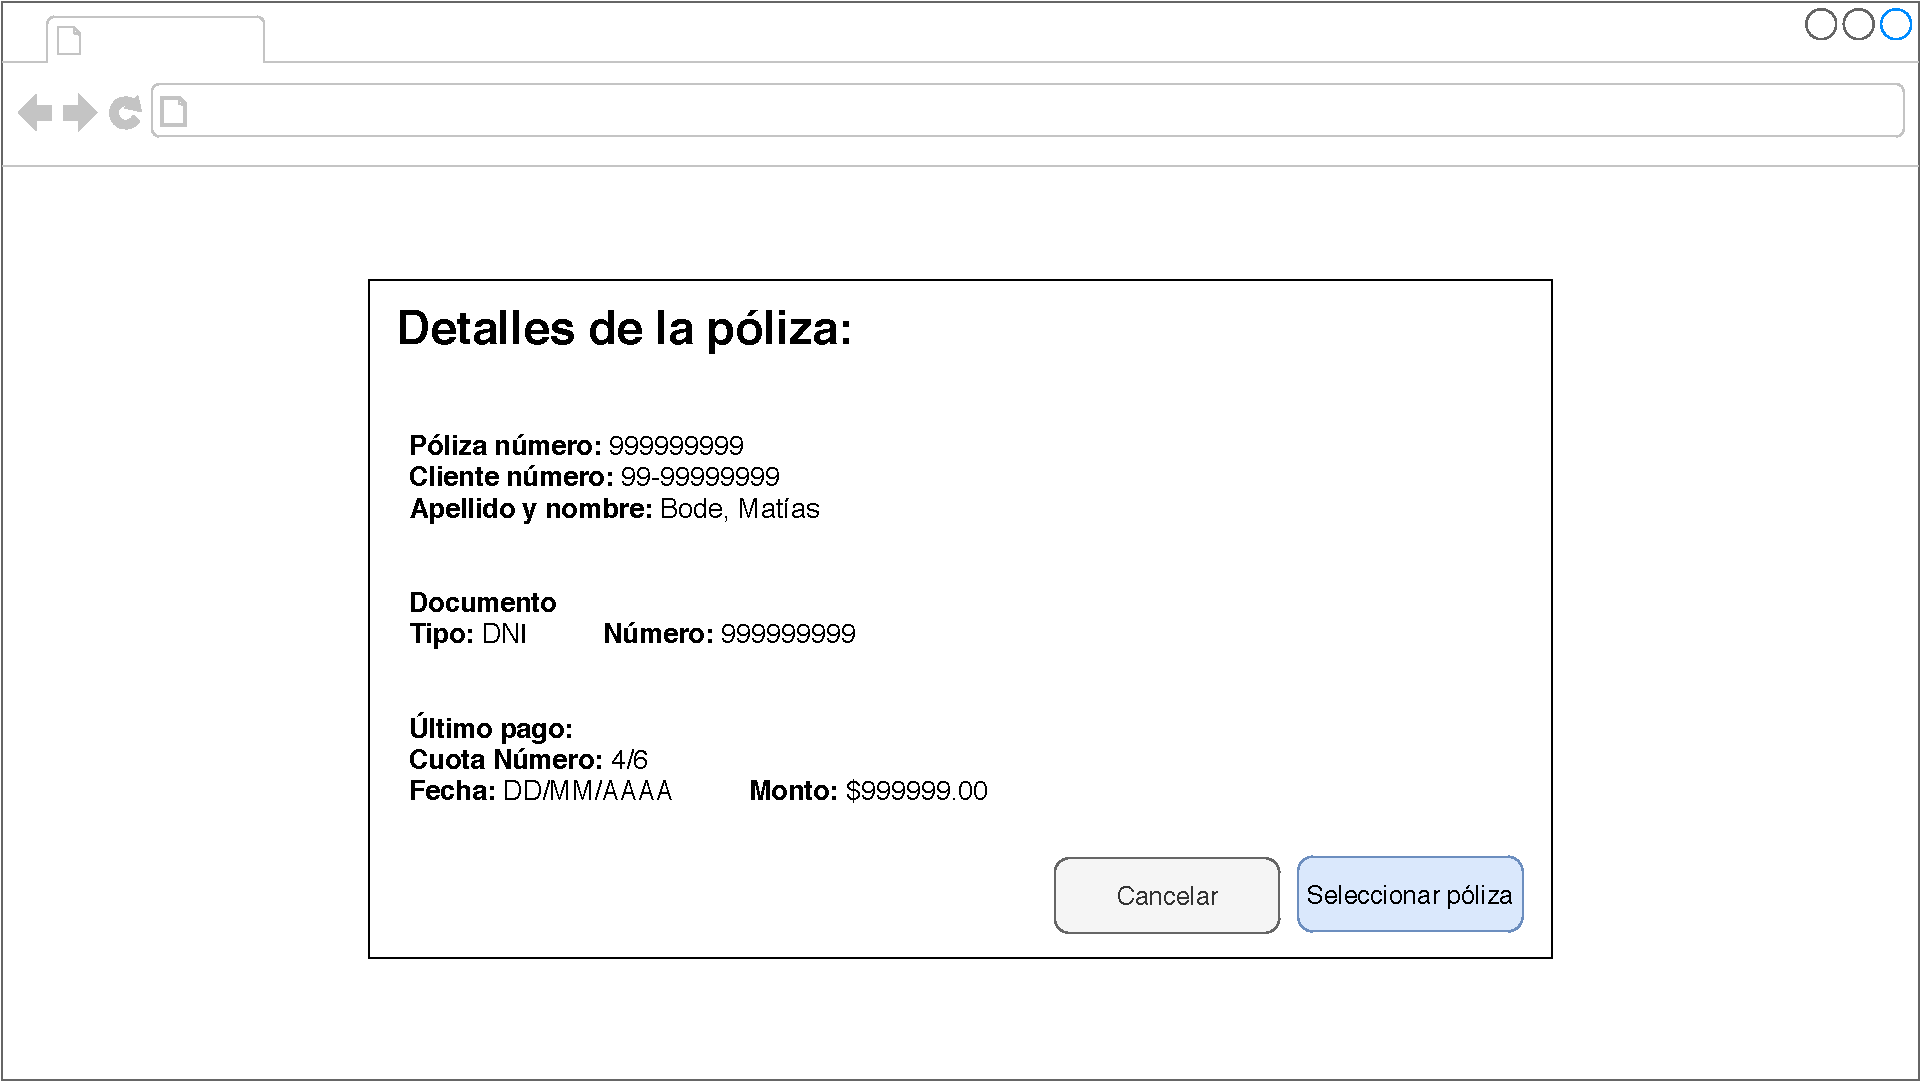
\includegraphics[width=\textwidth]{CU18/CU-183.pdf}
\caption{Caso de uso 18 (flujo principal)}
\end{figure}
\vfill



\end{document} 
